% !TEX root = "/expose_sebastian_keil/expose.tex"

\documentclass[12pt, oneside, paper=A4, DIV=15, ngerman]{scrartcl}
% \usepackage[english]{babel}

%for google fonts
\usepackage{parskip}
\usepackage{fontspec}
\setmainfont{Roboto}[
    Path=./font/Roboto/,
    Extension = .ttf,
    UprightFont=*-Regular,
    BoldFont=*-Bold,
    ItalicFont=*-Italic,
    BoldItalicFont=*-BoldItalic
    ]
\usepackage{float}

% \usepackage{fancyhdr}
% \pagestyle{fancy}
% \fancyhf{} % Clear all header and footer fields
% %\renewcommand{\headrulewidth}{0pt} % No horizontal line in header
% \fancyhead[C]{"Comparative Analysis of the BIWaM and ODOG Models: Identifying structural and behavioural differences and parallels" TBD} % Centered header text
% \newcommand{\helv}{\fontsize{7}{9}\selectfont}


% Setzt die Einrückung auf 2em, du kannst diesen Wert anpassen
\setlength{\parindent}{2em} 

\usepackage[english]{babel}
\usepackage[utf8]{inputenc}

% \usepackage{float} % For multiple figures in one
% \usepackage[caption = false]{subfig}

\usepackage{subcaption} % For multiple figures in one

\usepackage{graphicx} % For including images
\usepackage{caption} % For caption customization
\DeclareCaptionFormat{myformat}{\fontsize{10}{10}\selectfont#1#2#3}
\captionsetup{format=myformat}


% Schriftart
%\usepackage{arev}
%\usepackage[T1]{fontenc}

%Schriftart
%\usepackage{libertine}
%\usepackage{libertinust1math}
%\usepackage[T1]{fontenc}

% Mathe, Symbole, Einheitendarstellung, Chemie
\usepackage{siunitx}  

% Typographie
\usepackage[auto]{microtype}

% Autorenangaben
\usepackage[german]{authblk}
\renewcommand\Authand{, }
\renewcommand\Authands{, }

%Paket zur Erstellung von Gantt-Charts
\usepackage{pgfgantt}

% Darstellung der Literaturangaben
\usepackage[
backend=biber,
style=apa,
sortcites=true,
sorting=nyt,
% citestyle=apa,
% maxbibnames=2,
% firstinits=true
]{biblatex}

\setlength\bibitemsep{2\itemsep}


% Speicherort der Literaturangaben (*.bib Datei)
\bibliography{literatur/refs}

% pdf-Einstellungen
% Angaben ggf. aktualisieren!
\usepackage[
pdftitle={},
pdfsubject={},
pdfauthor={},
pdfkeywords={},  
% Links nicht einrahmen
hidelinks
]{hyperref}


\subject{Bachelor Thesis}
%\title{How the differences between the ODOG and BIWAM models are relating to other findings in vision research?}
\title{Comparison of two multiscale spatial filtering models}
\author[]{Sebastian Keil}
% \author[]{Dr. Joris Vincent}
\affil[]{TU Berlin, Computer Engineering B.Sc.}
\author[]{Supervisor: Dr. Joris Vincent}
\affil[]{TU Berlin, Computational Psychology}
% \affil[2]{TU Berlin, Computational Psychology, Marchstraße 23, 10587 Berlin}
\date{\today}

\begin{document}

\maketitle
\thispagestyle{empty}

%how to quote: ~\parencite{ebel2009}

\renewcommand*\contentsname{Summary}
\tableofcontents

\raggedright
\newpage

\setcounter{page}{1}
\section{Introduction}
\subsection{Light and the Visual System}

In the environment, light is emitted by a source of illumination, such as the sun. Any
surface on which this light falls will reflect a portion of it as \emph{luminance}. This
portion is called the \emph{reflectance} of the surface. The luminance is therefore the
result of \emph{illuminance} and reflectance, as shown in Figure
\ref*{fig:light_visual_system} a). A lightmeter can measure the amount of luminance
reflected by a surface, but it cannot tell what the reflectance of this surface is,
because the luminance could be the product of any combination of illuminance and
reflectance. \\
The formula in Figure \ref*{fig:light_visual_system} shows the problem from a mathematical
perspective. \(L\) represents luminance, \(I\) and \(R\) illuminance and reflectance,
respectively. It is simply impossible to solve for \(I\) and \(R\), when only \(L\) is
been measured, since for every \(R\) there is an \(I\) to produce the measured \(L\)
\parencite{adelson2000}. \\ 
However, the human visual system can solve this problem as seen in Figure 
\ref*{fig:light_visual_system}. It is also processing only luminance, yet it is able to
generate the perception of reflectance, which is referred to as lightness.

\begin{figure}[H]
\centering
\centering
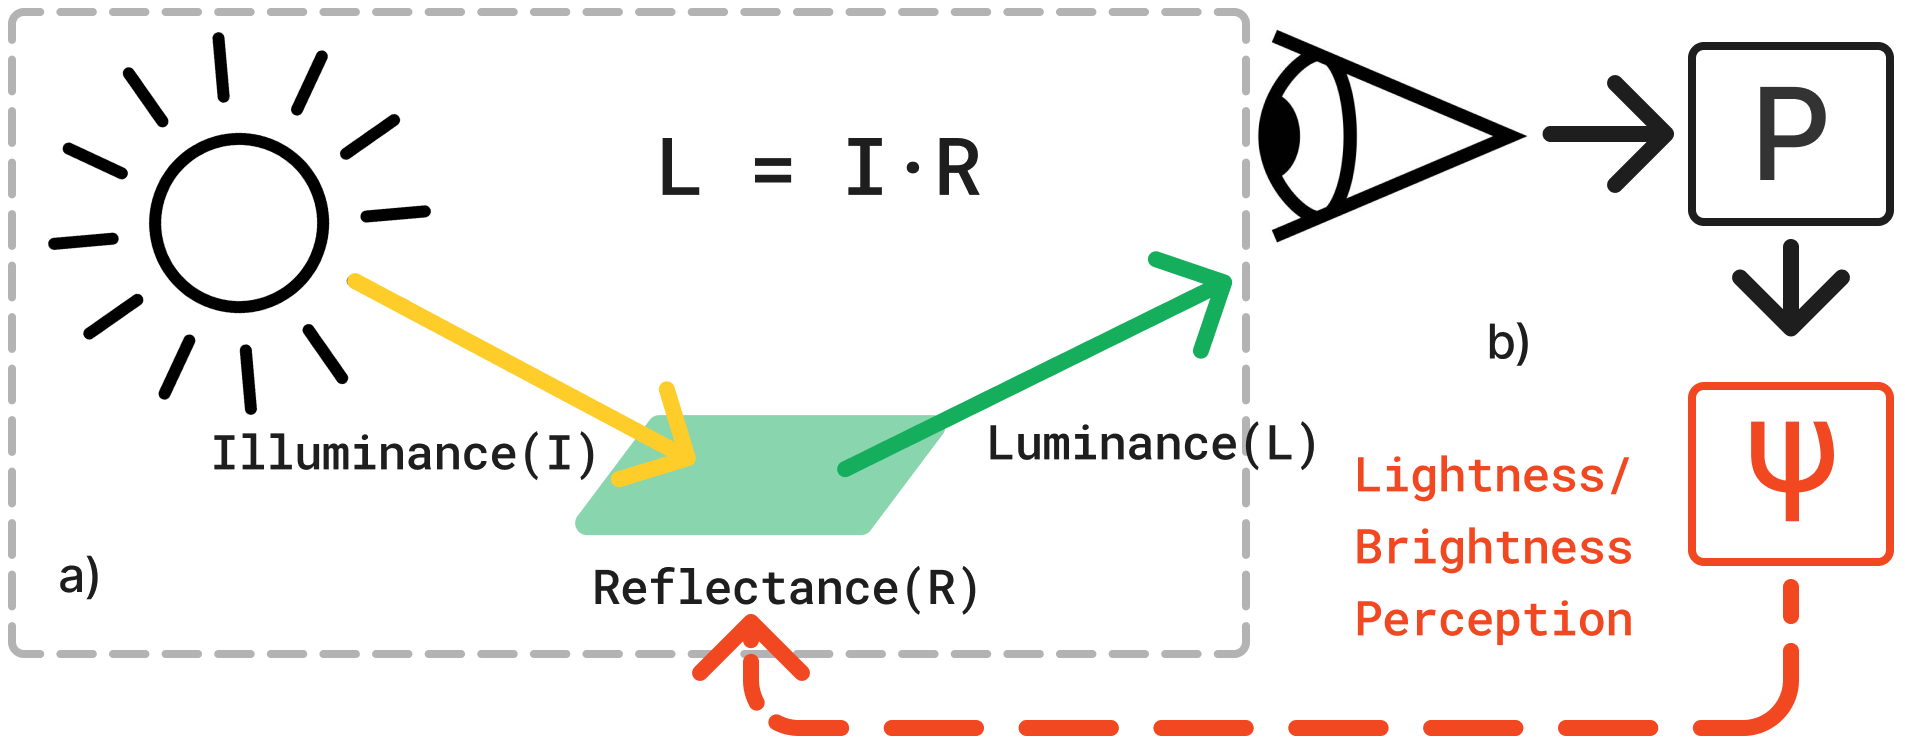
\includegraphics[width=0.9\textwidth]{media/lightness_color_formula.png}
\begin{minipage}{0.8\textwidth}
\caption[Relationship between illuminance, reflectance and luminance]{a) Relationship
between illuminance, reflectance and luminance. Luminance is the result of illuminance and
reflectance. b) The human visual system processes luminance through an unidentified
mechanism, represented by P which is determining lightness and brightness perception ψ of
the surface.}
\label{fig:light_visual_system}
\end{minipage}
\end{figure}

Next to lightness, humans also perceive brightness, which is the perception of luminance,
seen in Figure \ref*{fig:light_visual_system} b). Unlike reflectance, luminance is directly available
at the retinal image and brightness could in principle be derived from the retinal
measurement. However, the visual system does not only consider the corresponding
luminances when evaluating the perceived lightness and brightness of image areas, it also
takes into account the luminances of the surrounding regions \parencite{Kingdom1997}. As a
result the perception can differ from the actual retinal information. The mechanisms
through which the visual system accomplishes these tasks are the subject of current
research and will be discussed further in the following sections.
\newpage

\begin{figure}[H]
    \centering
    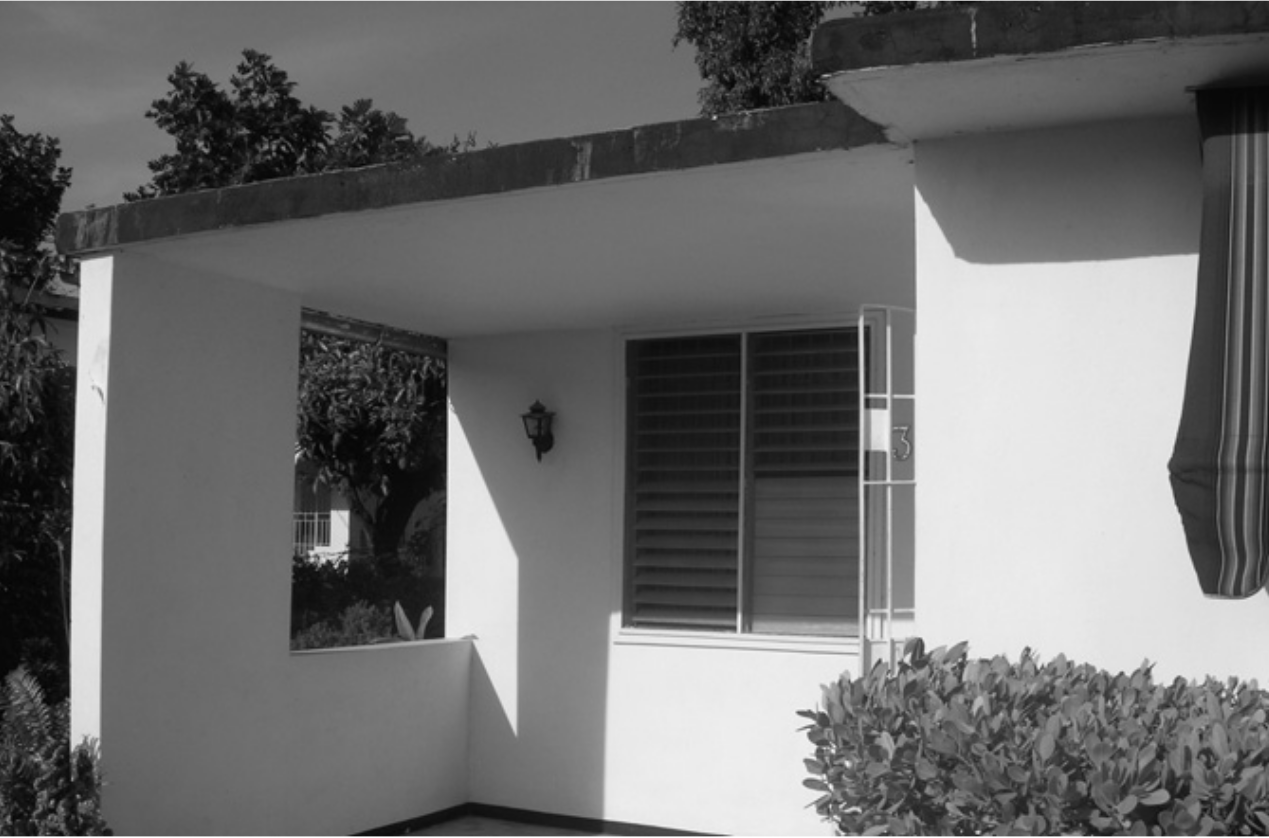
\includegraphics[width=0.7\textwidth]{media/bright_lightness.png}
    \begin{minipage}{0.8\textwidth}
    \caption[Lightness and brightness are distinguishable]{Lightness and brightness are
    distinguishable when illumination is visible. \emph{"The walls of the house appear
    uniformly white — a lightness judgment — yet are brighter in some places than others —
    a brightness judgment"}. Quote and picture from Kingdom \parencite*{Kingdom2014}.}
    \label{fig:figure2}
    \end{minipage}
\end{figure}


The distinction between lightness and brightness becomes apparent when information about
illumination is visible, as seen in Figure \ref*{fig:figure2}. \emph{"The walls of the
house appear uniformly white — a lightness judgment — yet are brighter in some places than
others — a brightness judgment"} \parencite{Kingdom2014}. This distinction is important
because brightness is about the relationship between the object and its environment. In
other words, it reveals how the object is exposed to illumination. Lightness, on the other
hand, represents the intrinsic properties of the object, such as color, regardless of the
environment.

Since reflectance is only implicitly perceivable, it can lead to uncertain situations. For
instance, a shadow can dim an area so that a white surface within the shadow reflects the
same amount of light as a black surface in full illumination next to it. Despite this,
human observers can usually distinguish between the white and the black surface
\parencite{arend1993}. 

This phenomenon is illustrated by Edward H. Edelson's \emph{checkerboard shadow illusion},
shown in Figure \ref*{fig:figure3}. The two patches A and B on the checkerboard in Figure
\ref*{fig:figure3}a appear to have different colors, even though they are emitting the
same light, as shown in Figure \ref*{fig:figure3}b.

The cylinder seems to cast a shadow, even though there is no real light source, since the
image is just a two-dimensional representation of the scene. However, the visual system is
designed to process images coming from three-dimensional scenes with illumination and
shadows and so it processes the checkerboard shadow illusion with all the available
information about depth and illumination. To logically follow the processing, one can say,
that patch B reflects the same amount of light as patch A (seen in Figure
\ref*{fig:figure3}b), but is located in the shadow of the cylinder and therefore must have
a higher reflectance. In other words, the visual system needs to react to differences in
illumination and compensate for them in order to estimate the reflectance. This behavior
ensures that the perception of a scene is closely related to the reflectance of its
surfaces and is largely unaffected by the illumination. 

\begin{figure}[H]
    \centering
    \centering
    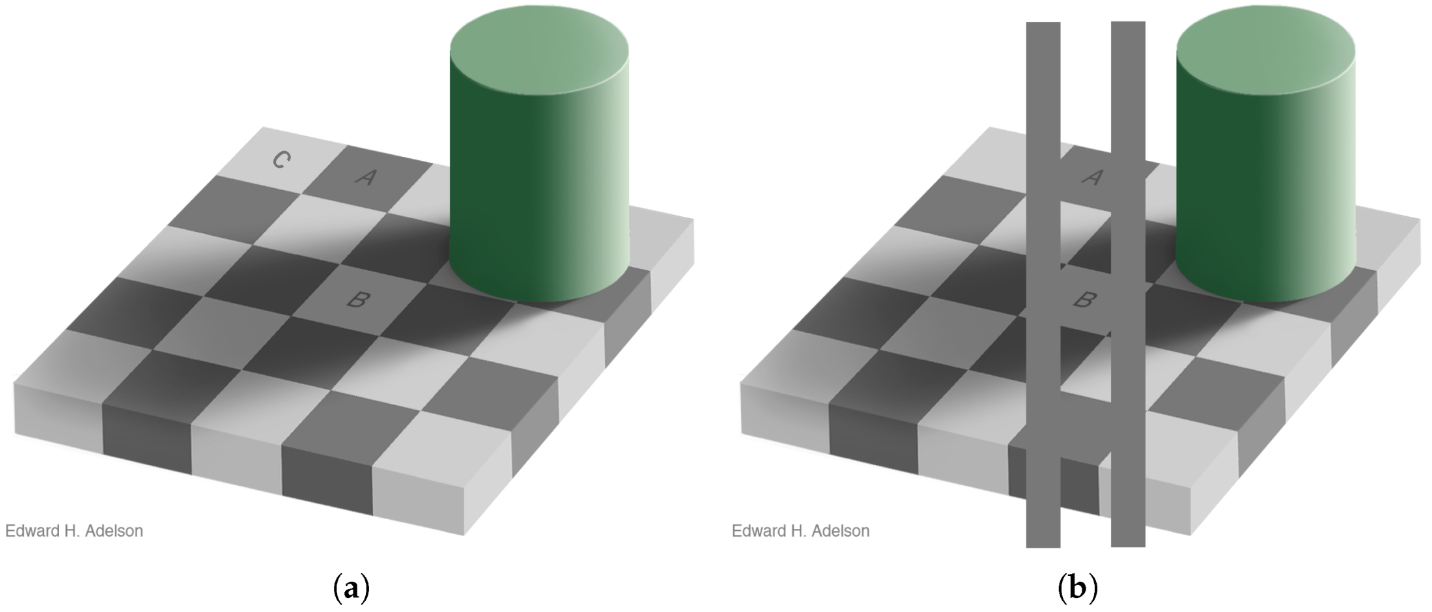
\includegraphics[width=0.85\textwidth]{media/checkershadow_double_full_.png}
    \begin{minipage}{0.8\textwidth}
    \caption[Checkerboard shadow illusion]{(a) The Checkerboard shadow illusion image; (b)
    proof image \parencite{adelson1995checkershadow}.}
    \label{fig:figure3}
    \end{minipage}
\end{figure}

In everyday life, illusions in brightness and lightness perception are rare, likely due to
the vast amount of information that the visual system can make use of. Shading, shadowing,
and spatial depth can guide the perception of brightness and lightness, like in the
checkerboard shadow illusion. However, there are illusions with less information available
for the visual system, which need a different explanation.

\subsection{Low-Level Vision}

One very simple illusion is the classic \emph{simultaneous contrast illusion}, as seen in
the upper part of Figure \ref{fig:figure4}. Two identical grey squares appear to be
different in brightness, depending on their surroundings. The lack of information about
illumination and spatial depth is crucial in comparison with the checkerboard shadow
illusion. The parts of the visual system, which are processing illumination or spatial
depth, will have no information available in the simultaneous contrast illusion. Here the
idea of detecting illumination and compensating for it will fail, hence a different
explanation is needed.

An explanation for the simultaneous contrast illusion is offered by neural units in the
retina. Hering (1834 —1918) was the first describing their \emph{center surround fields},
which compare luminance areas with their surrounding areas. With that
they could account for the simultaneous contrast illusion. The lower part in Figure
\ref{fig:figure4} illustrates the principle. The blocks under the illusion represent
neurons responding to areas of the illusion image. The surrounding blocks subtract and the
center block adds their responses to the fourth block underneath. When the surrounding
blocks are sensing the darker surrounding of the left patch, their response is small and
so the subtraction is small. As a result the left summing block receives a higher
response, correlating with a human observer experiencing the left patch to be brighter. On
the right patch the surrounding blocks are sensing bright surroundings and so the
subtraction is higher and the summing block receives a lower response, also correlating
with a human observer experiencing the right patch to be darker.


\begin{figure}[H]
    \centering
    \centering
    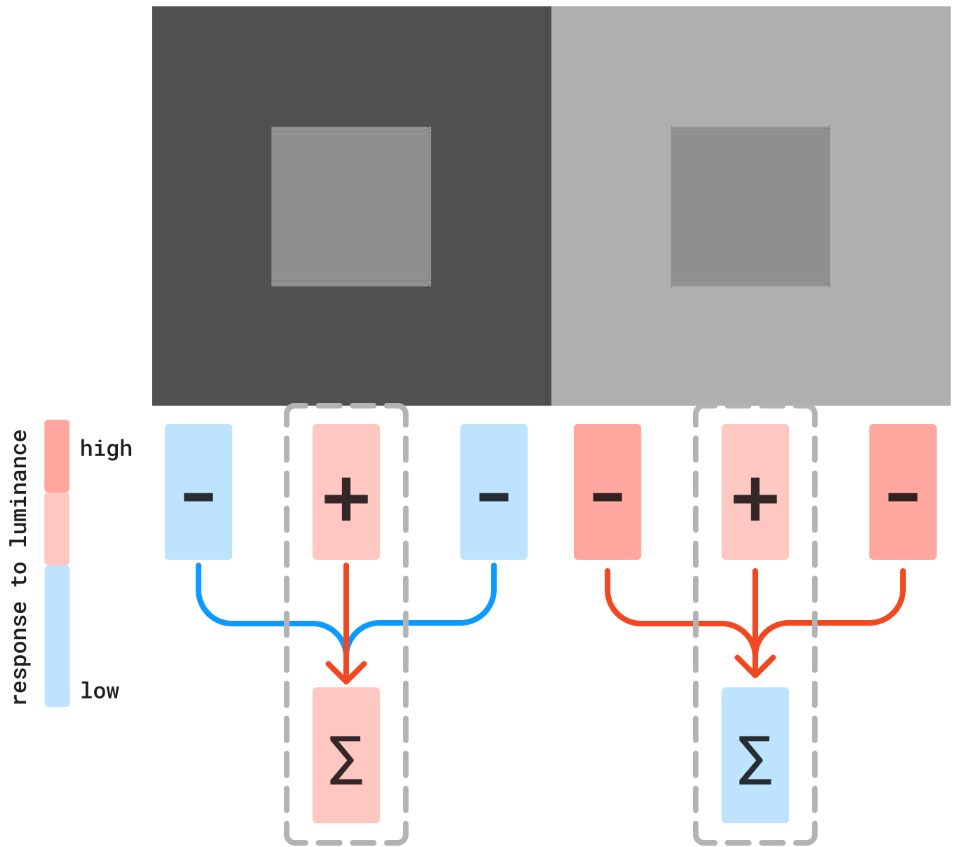
\includegraphics[width=0.75\textwidth]{media/centre_surround.png}
    \begin{minipage}{0.8\textwidth}
    \caption[The principle of center surround fields]{Above: The simultaneous contrast
    effect. Two identical grey patches appear to be different in brightness, depending on
    their surrounding. The left patch appears brighter than the right patch. \\ Below: The
    principle of center surround fields. The blocks on each side represent neurons, where
    the surrounding blocks subtract and the center block adds their responses to the
    fourth block underneath. On the left side the center response is medium (light red),
    corresponding to the left patch in the illusion, while the surround response is low,
    corresponding to the surrounding dark gray in the illusion. The summation results in a
    medium response. On the right side the center is the same, but the surround response
    is higher (dark red) and so the summation in the fourth block is lower. The responses
    of the patches in the illusion depends on their surrounding.}
    \label{fig:figure4}
    \end{minipage}
\end{figure}


Simple mechanisms like the center surround fields could be responsible for human
brightness perception\footnote{The terms brightness and lightness become synonymous
without information about illumination and will be used interchangeably in the following
sections, as we will discuss only such illusions}. They exist in different sizes and
their outputs are also interacting with each other. This complex neural processing
results in so called \emph{sensory channels}, where each channel is selectively sensitive
to different sizes of contrast areas, also referred to as spatial frequencies
\parencite{Sachs71}. Large center surround fields will respond to low spatial frequency
information like large objects and gradual changes across the image. Small center surround
fields will respond to high spatial frequency information like fine details and edges.\\
The organization of center surround fields can isolate specific image properties and the
interaction of their outputs provides a mechanism to process the retinal information in a
much more meaningful way. This has inspired researchers to investigate the computational
modeling of center-surround fields and their interactions.


\subsection{Modelling Human Vision}

The basic idea of center surround fields is to compare luminances with their surround
luminances. Since computers handle image data as discrete pixel values, it is
mathematically straight forward to model this comparison with algorithms. A common
approach is to design a convolution filter, representing the center surround field and
convolve it with the image pixel values. In Figure \ref{fig:figure5} the principle of a
convolution on a grayscale image is shown. The filter values are applied on the input
pixels by an element-wise multiplication. In the example of Figure \ref{fig:figure5} the
filter is comparing every pixel with its direct neighboring pixels.

\begin{figure}[H]
    \centering
    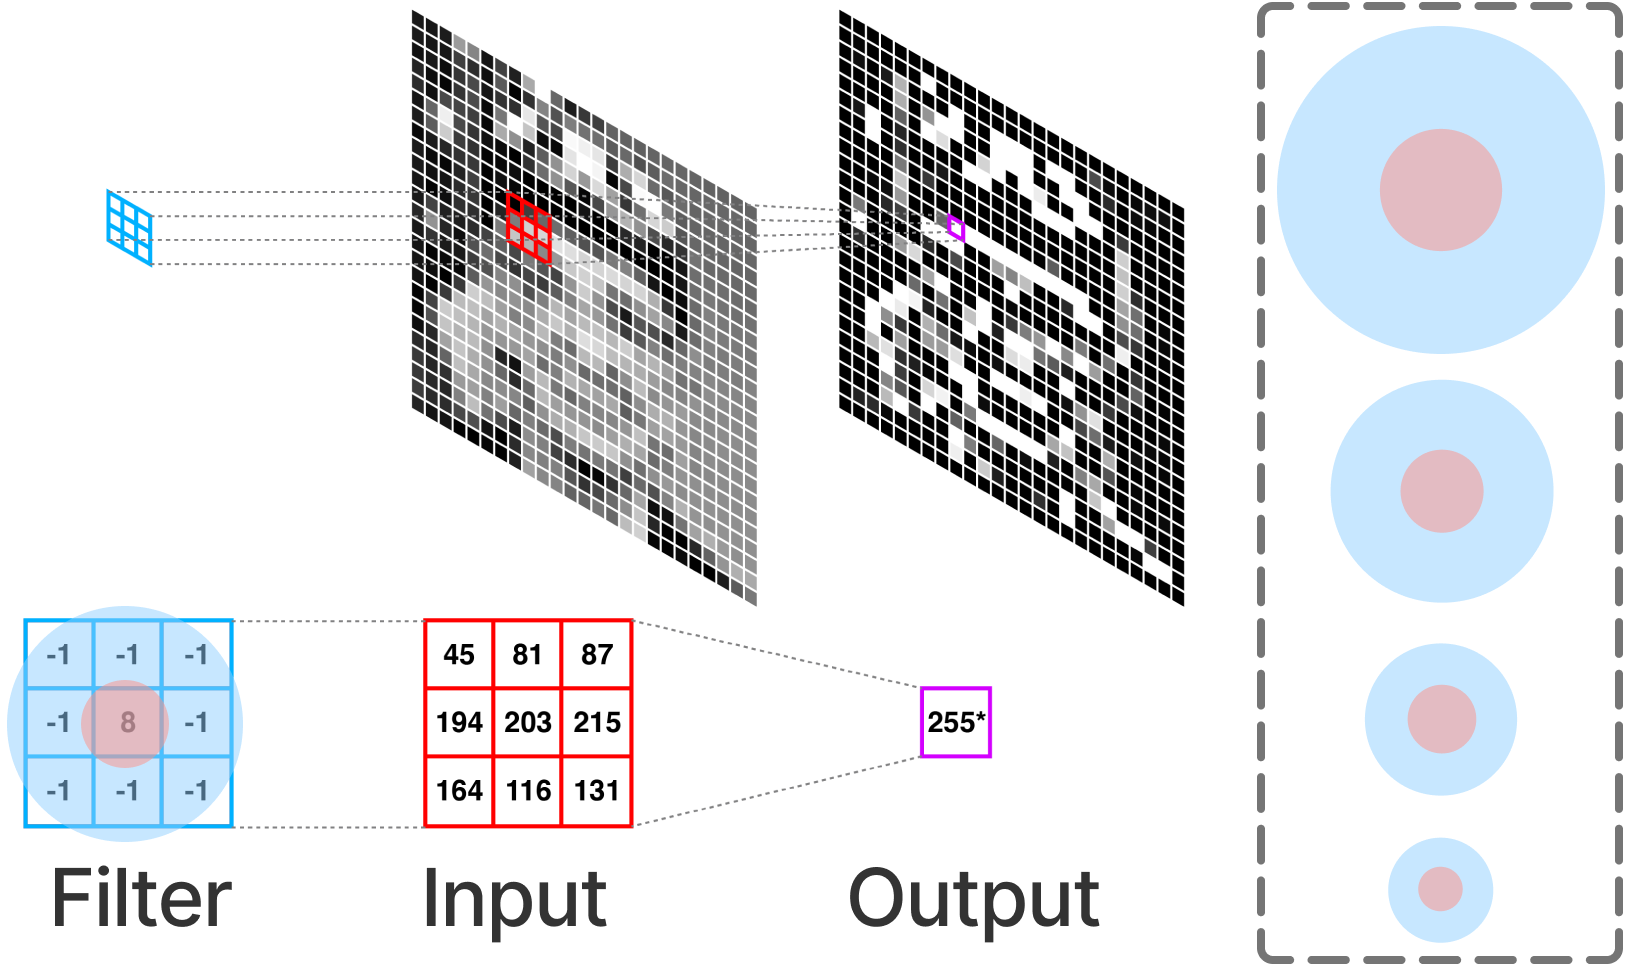
\includegraphics[width=0.7\linewidth]{media/convolution.png}
    \begin{minipage}{0.8\textwidth}
    \caption[Applying a convolution on an image]{ Applying a convolution on an image is a
    common approach to model center surround fields. 
    % The convolution works by sliding a filter over an image and computing
    % the sum of element-wise multiplications to generate the output pixel. 
    Every pixel of the input image is multiplied with the center value of the filter (8)
    and then summed up with every surround pixel multiplied with the corresponding value
    in the filter (-1). The resulting sum is the new pixel value for the output image at
    the position of the original pixel. the left Figure is inspired by Gundersen
    \parencite*{Gundersen2017}. The right side shows a filterbank, existing of multiple
    filters in different sizes.}
    \label{fig:figure5}
    \end{minipage}
\end{figure}

To address the benefits of different sized center surround fields of the retina, it is
sufficient to create multiple filters of varying sizes. On the right in Figure
\ref{fig:figure5} a so called filterbank is shown. Each of the different sized filters
will be applied on the input image and generate its own output, similar to the sensory
channels of the visual system. Larger filters will compare more pixels and will respond
stronger to low spatial frequencies. Smaller filters will respond to high spatial
frequencies. The outputs from all the filters of a filterbank are representing the image
information decomposed by frequencies. In order to reconstruct the image, it is sufficient
to sum the filter outputs. The reconstructed image is identical to the original
image, since all information is kept during the process.

To replicate human perception the DOG (Difference Of Gaussian) model from Blakeslee and
McCourt does a reweighting of the filter outputs before reconstruction
\parencite{Blakeslee1997}. Inspired by the contrast sensitivity function of the human
visual system, it attenuates lower frequencies. As a consequence the output image is no
longer identical to the input image. In fact for the simultaneous contrast illusion the
left patch is brighter and the right patch is darker, aligning with the human perception
of the illusion.

\newpage

\begin{figure}[H]
    \centering
    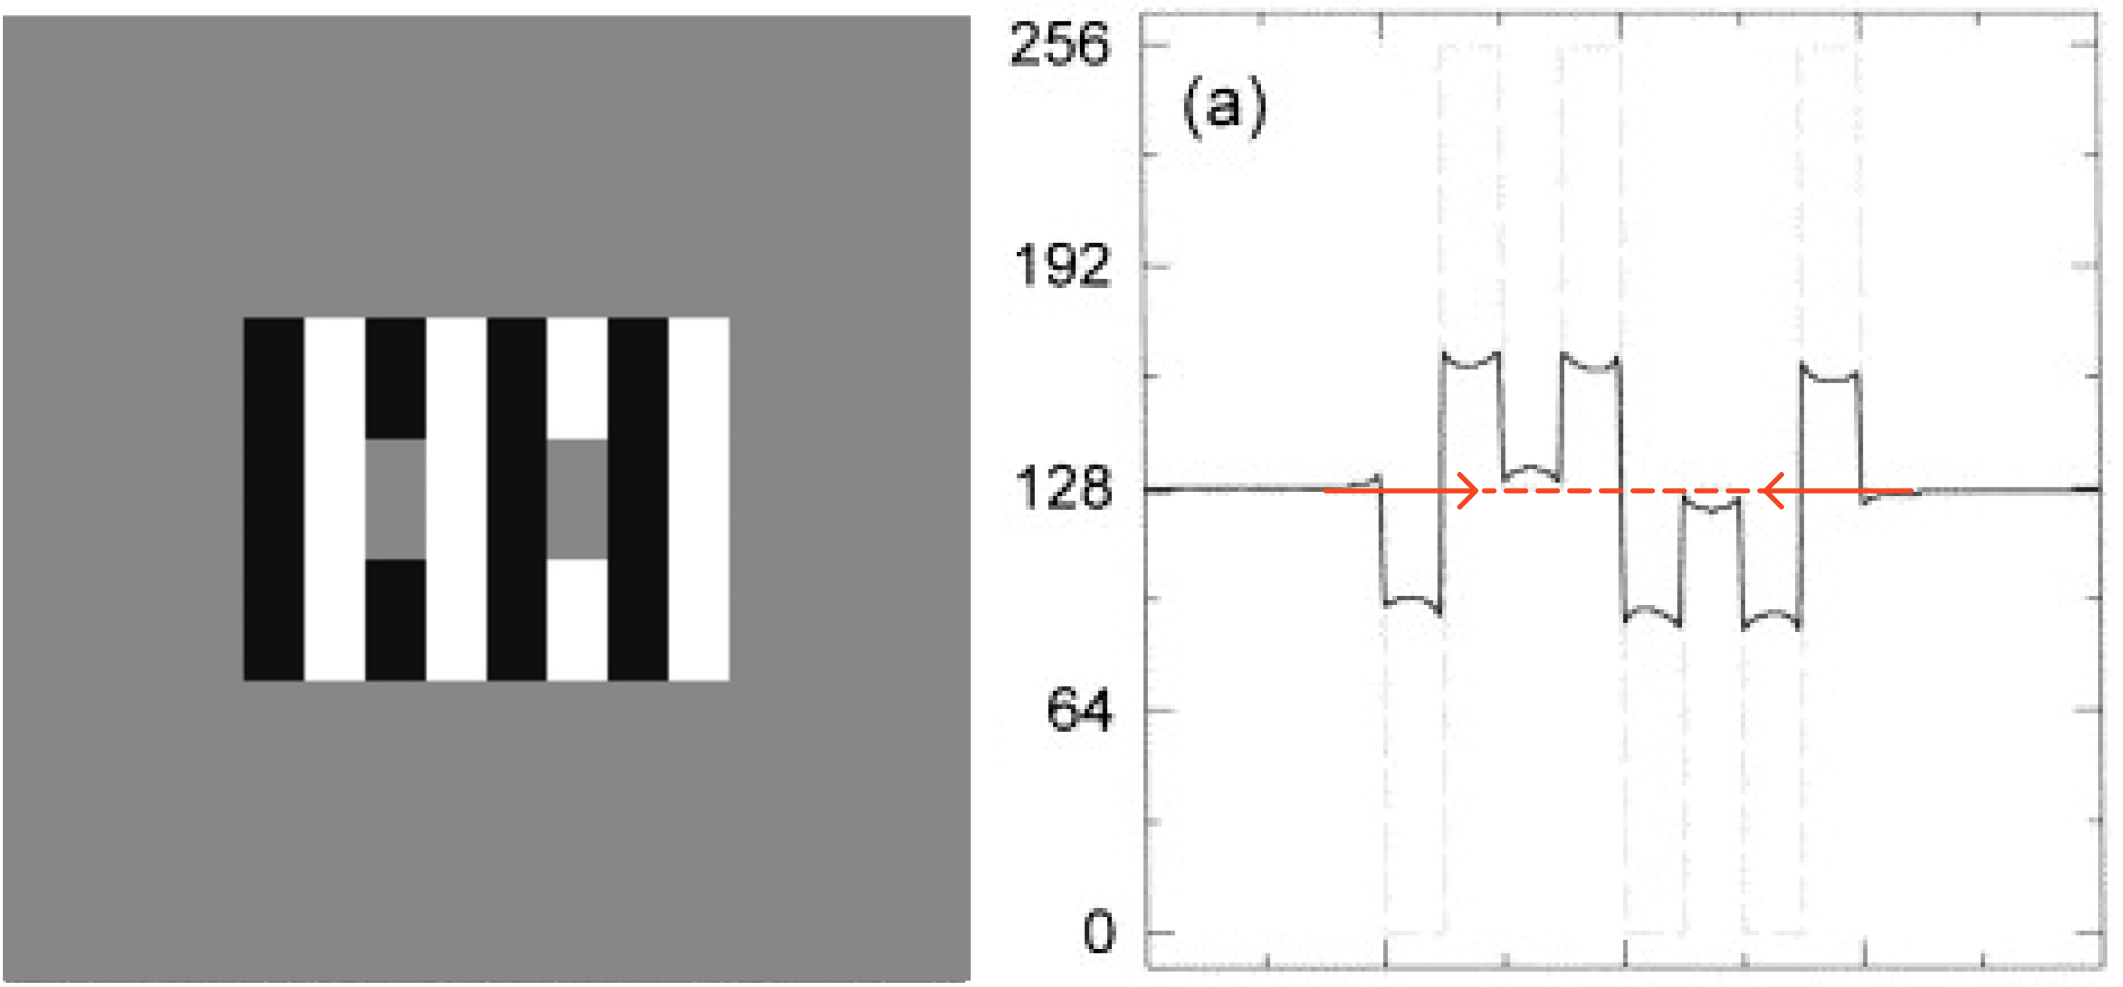
\includegraphics[width=0.7\linewidth]{media/whites_effect_model.png}
    \begin{minipage}{0.8\textwidth}
    \caption[Models response to White's Effect]{In White's Effect (left) the shift in
    perceived brightness is in the opposite direction compared to brightness contrast.
    Both patches are identical, but the left patch on the black bar appears to be brighter
    than the patch on the white bar, even if it shares most of its edges with white
    surfaces \parencite{Whit1979}. The diagram on the right shows the processed White's
    Effect illusion by the ODOG model. The dashed line refers to the luminance profile
    across the horizontal center of the illusion. The solid line represents the models
    output along the same line. The red markers indicate that the models output is in
    accord with the human perception \parencite{Blakeslee1999}.}
    \label{fig:figure6}
    \end{minipage}
\end{figure}

The reweighting between decomposition and reconstruction appears to be a key mechanism of
the DOG model making it capable of replicating human perception of the simultaneous
contrast illusion. However, the DOG model cannot account for all brightness phenomena. For
instance, the White's effect, illustrated on the left side of Figure \ref{fig:figure6},
cannot be explained by Blakeslee and McCourt's initial model. One year later, in 1999,
they developed an extended version of the model, called ODOG (Oriented Difference Of
Gaussian), which can account for White's effect shown on the right side of Figure
\ref{fig:figure6} \parencite{Blakeslee1999}. Two changes are responsible for its new
capabilities. They extended the filterbank by six different orientations for each filter,
therefore they also changed the isotropic filters of the DOG model to anisotropic filters
in order to be able to rotate them. The second change is a normalization step before
reconstruction. The ODOG model will be discussed in more detail at a later point in the
thesis. \\
The ODOG model became very famous and inspired a whole family of so-called spatial
filtering models. Among them is a model with a different approach, the BIWaM (Brightness
Induction Wavelet Model) model from Otazu. It doesn't use a filterbank to decompose the
image, but rather convolves its filters within a wavelet transformation
\parencite{Otazu2008}.


\subsection{ODOG and BIWaM}

ODOG and BIWaM are oriented spatial-filtering models, highlighting the importance of
low-level vision. Both models process an input image using filters, which are inspired by
the center surround fields. As shown in Figure \ref{fig:figure7}, their processing begins
with the decomposition of the input image (Step 1), using spatially scaled and oriented
filters. Each filter results in an channel that extracts specific orientations and
spatial frequencies of the image. The channels are then processed (Step 2) by reweighting
and normalization, each model has it own strategy. In the final step (Step 3) all outputs
are merged to reconstruct the output image.

\begin{figure}[H]
    \centering
    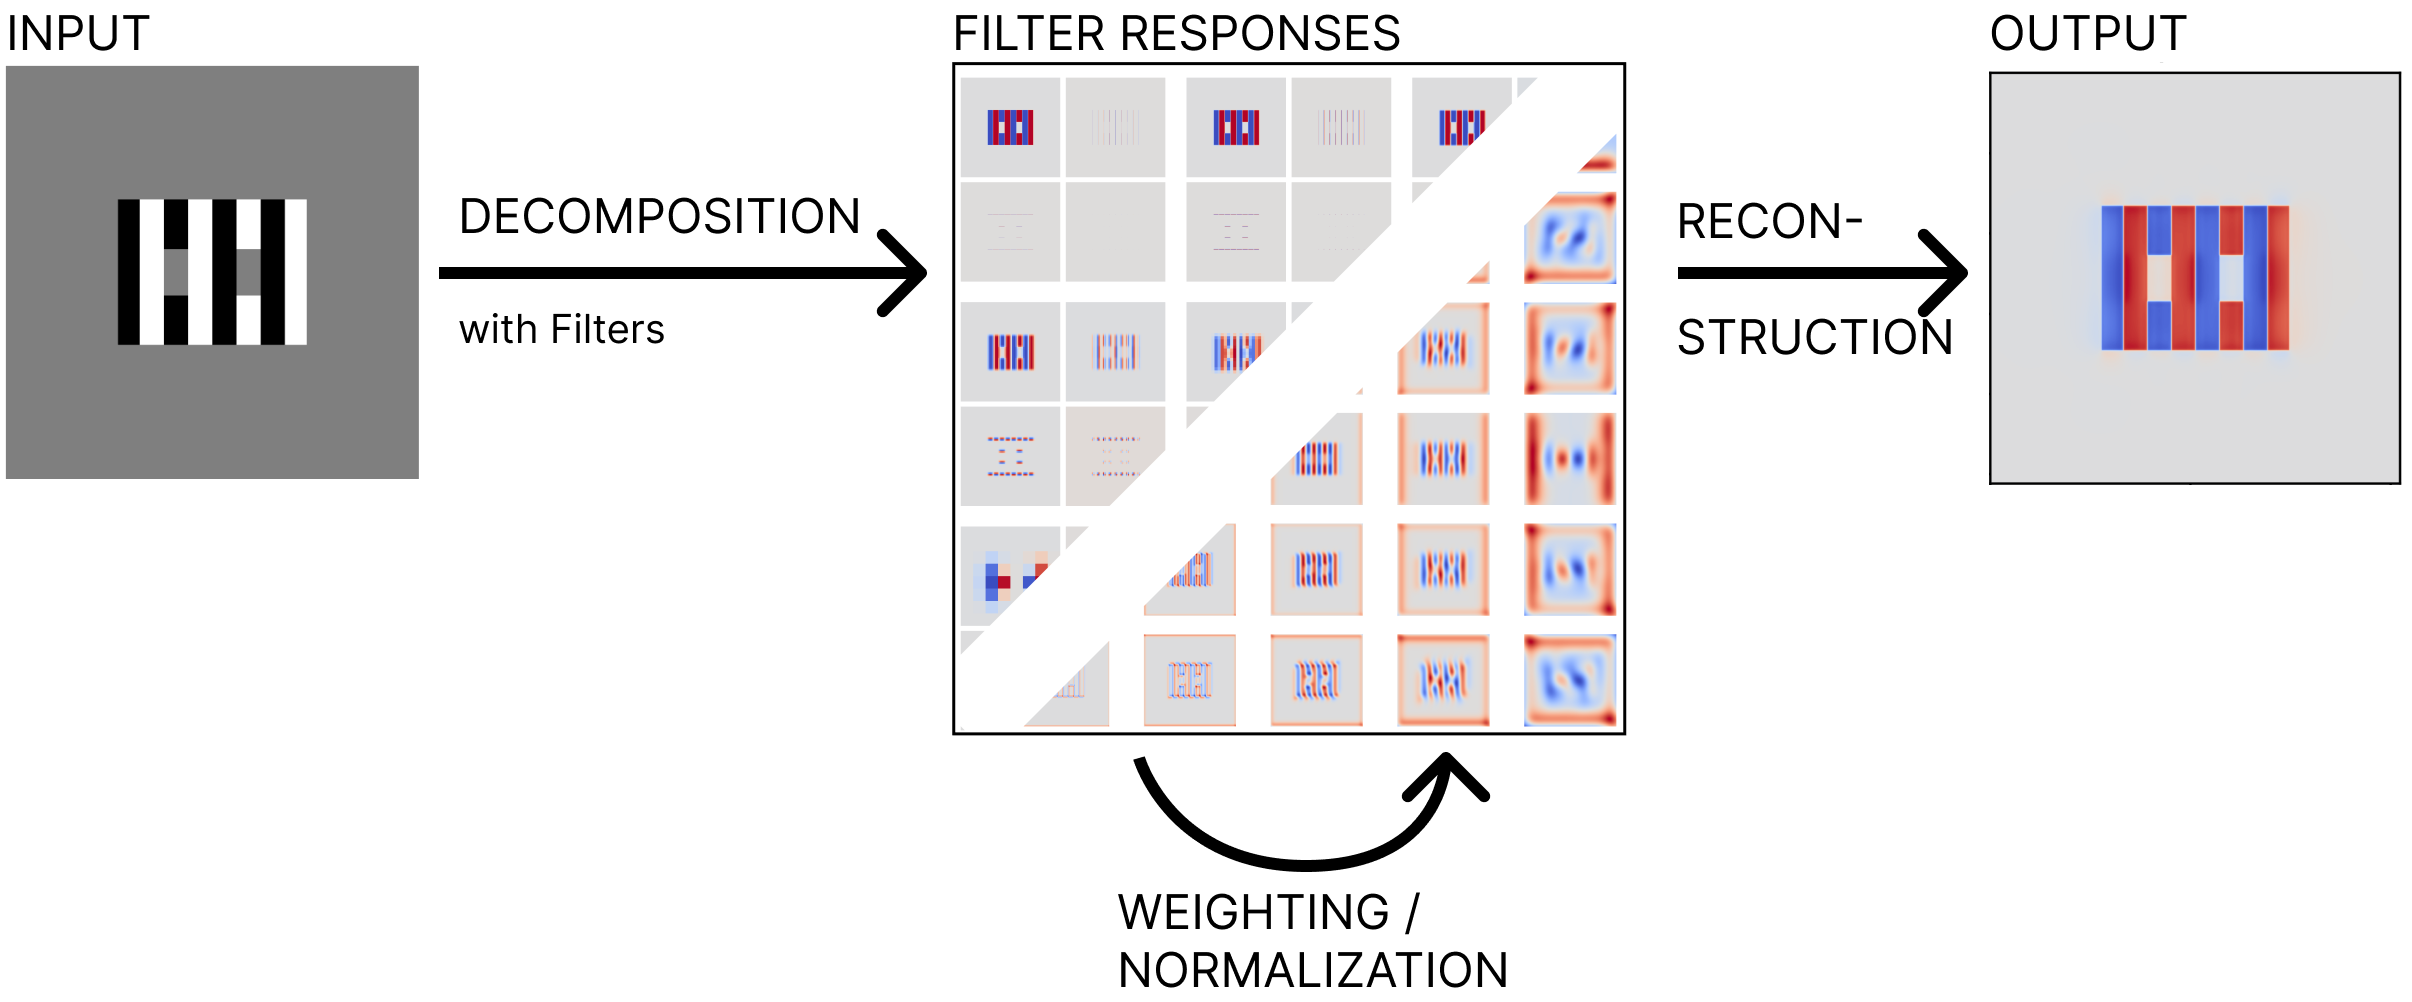
\includegraphics[width=\linewidth]{media/methodology/models_overview.png}
    \begin{minipage}{0.7\textwidth}
    \caption[Structural overview of models]{Structural overview of ODOG and BIWaM models, three steps to analyze}
    \label{fig:figure7}
    \end{minipage}
\end{figure}

The ODOG model uses a filterbank consisting of 42 filters in seven different scales and
six different orientations. Each filter convolves with the input image, extracting
frequency-specific and orientation-specific information. The outputs of the filters within
the same orientation are summed, with weights that are determined by the spatial
frequency. Lower frequencies receive smaller weights than higher frequencies, similar to
the contrast sensitivity of the visual system. These responses are normalized by their
root-mean-square energy, which is computed across all pixels and summed to yield the model
output. As a consequence of the response normalization, orientations with little energy in
the input image will have a proportionally larger influence on the model output
\parencite{Betz2015}.

In contrast, the BIWaM model uses wavelet transformation for decomposition instead of a
filterbank. This wavelet transformation also performs convolutions with filters of
different scales and orientations. It iterates through the decomposition 7 times
recursively, downscaling the image at each iteration but using the same spatially sized
filter. Therefore, it generates channels for different filter-to-image scales in each
iteration, similar to the filterbank in the ODOG model. The BIWaM model reweights channels
also based on a CSF-inspired function. The normalization across channels is localized,
using factors specific to contrast for every image region. This could be a main difference
between the models \parencite{Betz2015}. In the final step, the BIWaM model merges the
filter outputs to generate the output image.

\textcolor{red}{(TODO: write more about the models)}


At first glance, ODOG and BIWaM may seem conceptually distinct due to their differing
implementations. ODOG utilizes a filterbank, global CSF weighting, and separate
normalization across channels, while BIWaM employs wavelet decomposition, integrated
CSF-weighting, and localized normalization. However, both models share
a common conceptual framework: decomposition into orientation- and scale-specific
channels, weighting by the CSF, and interactions between channels. This raises the central
question of this thesis: Are ODOG and BIWaM fundamentally distinct models, or are they
merely different implementations of the same underlying conceptual idea? 


% Spatial filtering models are providing insights in the field of vision research and come
% with advantages and disadvantages. On some images the choice of the model can make a
% significant difference(TODO: Example). But these differences in model behavior are not
% trivial. To better understand the models algorithmic and the resulting effects, i plan to
% study two the models ODOG and BIWaM, which are known for... (TODO: why these models?). 
\newpage


\section{Methodology}

The aim is to determine whether these models are fundamentally distinct or represent
different implementations of the same conceptual idea. To achieve this, I will
systematically explore the conceptually corresponding parameters and mechanism of each
model for each stage (decomposition, weighting and normalization). For example in the
decomposition stage both models implement a corresponding parameter to define the scales
of the filters used to extract frequencies (ODOG: 'scales'; BIWaM: 'levels'). The plan is to
change the corresponding parameters at implementation level, to see if the resulting
changes in the model prediction correspond. If the models really only are different
implementations of the same idea a change of the corresponding parameters in both models
should result in similar changes in the predictions.

Given the iterative nature of this methodology, the thesis will not follow a traditional
methods-and-results structure. Instead, it is organized into five interdependent sections,
each correlating with a distinct processing stage of the models.

At the beginning of each section, an overview similar to Figure \ref{fig:figure8} will
provide a roadmap for the chapter, ensuring a clear narrative. Results from all sections
will be linked in the Discussion chapter, where I will comprehensively compare the models
and draw conclusions about their behavioral and structural relations. 

\begin{figure}[H]
    \centering
    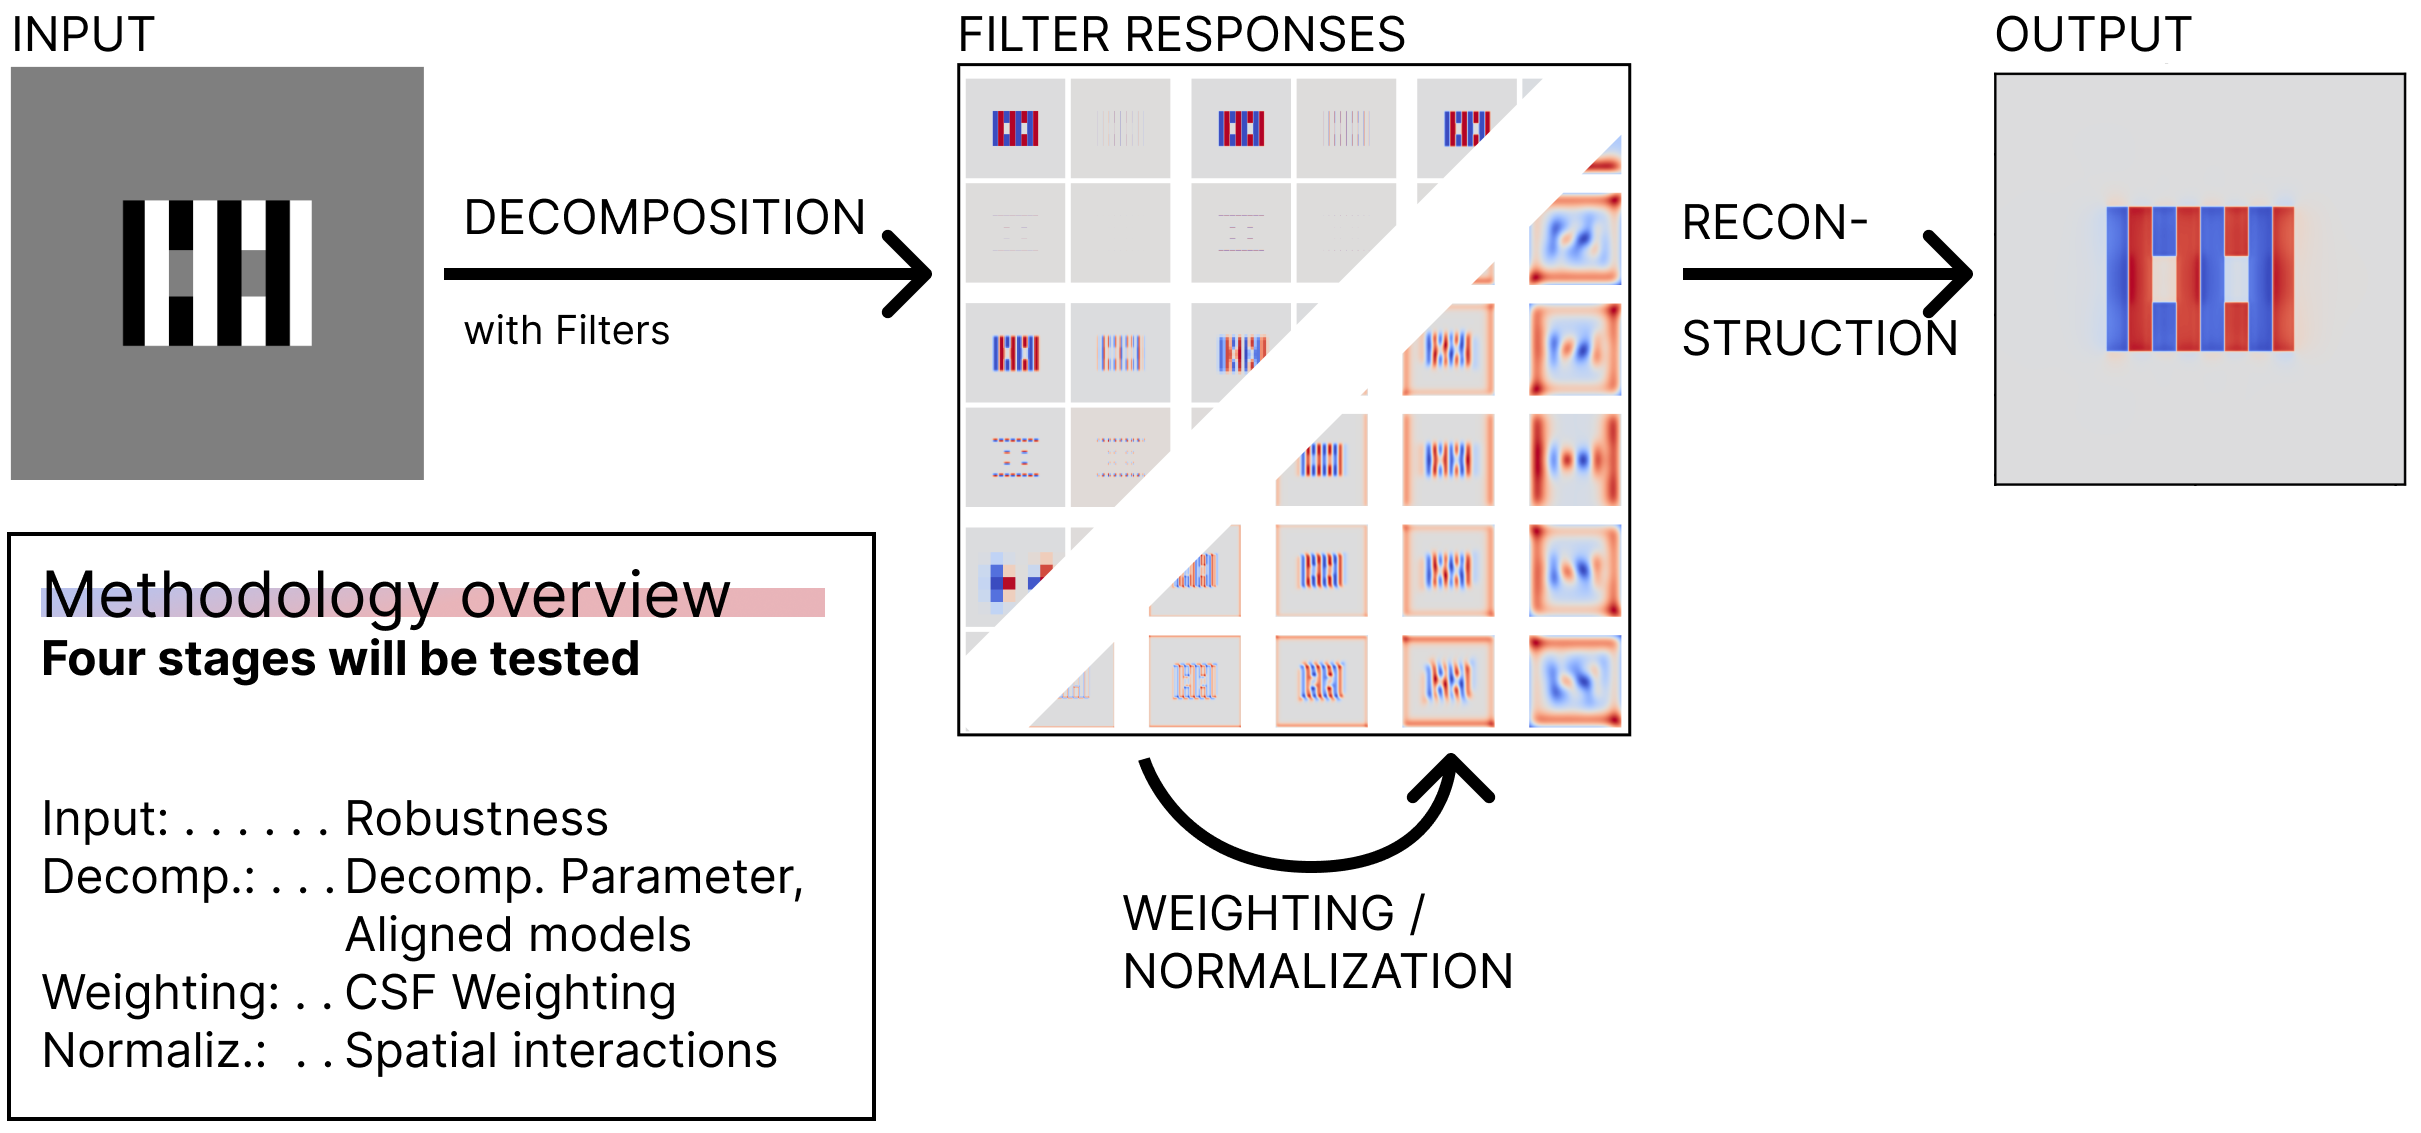
\includegraphics[width=\linewidth]{media/methodology/methodology_overview.png}
    \begin{minipage}{0.8\textwidth}
    \caption{Methodology overview of analysis}
    \label{fig:figure8}
    \end{minipage}
\end{figure}

By systematically testing conceptually corresponding parameters across the models and
stages, this methodology establishes a framework for exploring whether ODOG and BIWaM are
distinct models or different implementations of the same conceptual idea.


\subsection{Stimuli}
Both models are tested on a set of seven different stimuli. The variety in stimuli lowers
the risk of drawing conclusions based on specific features of a single stimulus and
provides a robust baseline for comparison in the next chapters. The stimuli used are: Two
versions of Whites effect, two versions of Simultaneous Brightness Contrast (SBC),
Checkerboard illusion, Circular Whites effect and the Dungeon illusion. The Dungeon
illusion is specifically chosen, because the authors of the BIWaM model mentioned, that
their model will account for it, while it was previously unexplained
\parencite{Otazu2008}. A List of all stimuli is shown in Figure \ref{fig:figure9}. \\
\textcolor{red}{(TODO: tell more about the stimuli, why these?)}

\textcolor{red}{(TODO preparation for section 2.2: which stimuli are new to the
models, which have been shown to be not working for a model?)}

This baseline focuses on the qualitative patterns of the models' responses rather than a
quantitative statement, as the models differ in architecture and output units. Running
identical stimuli through both models, which has not been done before, serves as the first
step in understanding their behavior. 

As expected, the predictions from the two models vary, reflecting their distinct designs.
The following chapters will analyze and compare their outcomes on this shared baseline.

\begin{figure}[H]
    \centering
    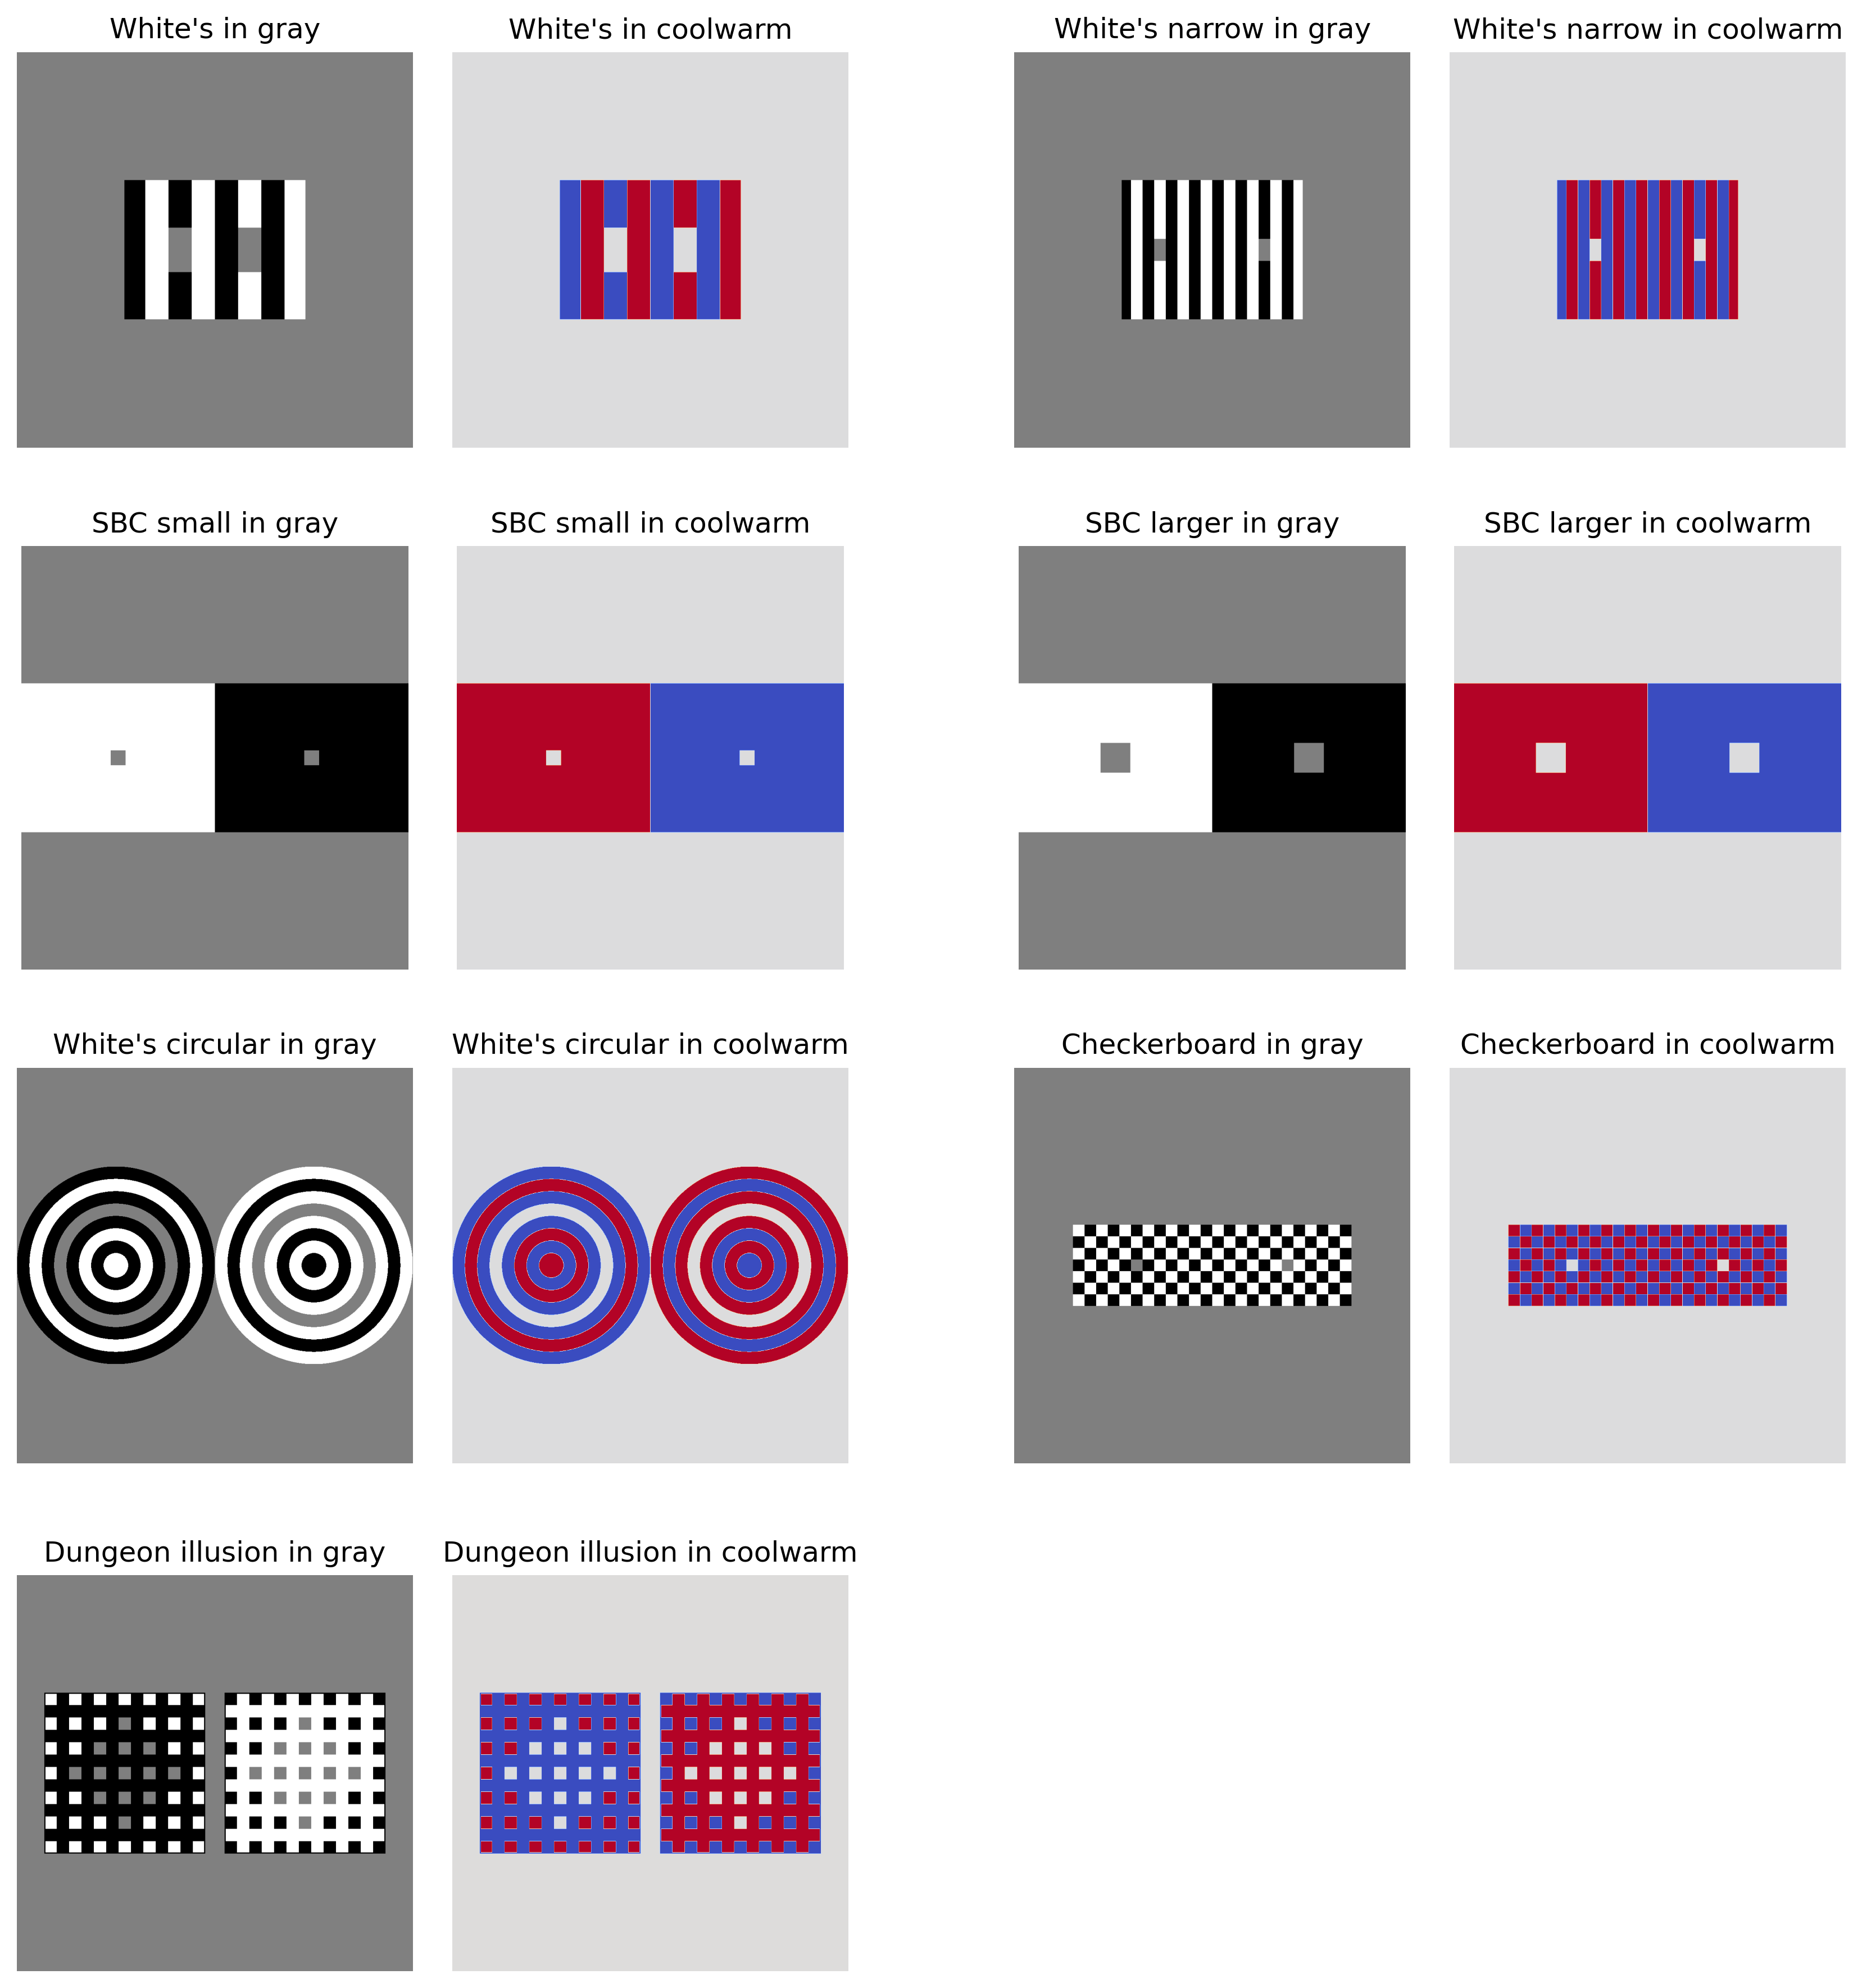
\includegraphics[width=\linewidth]{media/methodology/stimuli.png}
    \begin{minipage}{\textwidth}
    \caption[Overview 7 different stimuli]{The seven stimuli used to test the models are
    shown here, each displayed in greyscale and in the coolwarm colormap. Each stimulus
    consists of a black-and-white configuration where two targets, physically identical in
    their gray value, are embedded. The greyscale presentation generates a perceptual
    illusion in which one target appears brighter than the other due to its surroundings.
    However, the coolwarm colormap confirms the physical similarity of the targets by
    visually representing their identical intermediate gray value.}
    \label{fig:figure9}
    \end{minipage}
\end{figure}

\newpage

\subsection{Model responses}
% To create an initial baseline of the model responses, where I can refer to later, when I
% make changes in the models implementations, I ran both models on the set of stimuli shown
% in Figure \ref{fig:figure9}. However, as described in the previous section, some of the
% stimuli chosen for this thesis are not tested by the authors of the models or it has been
% shown that the a model can not account for some of the stimuli. To provide a better
% overview, i will not show all of the model responses here, but i will put them in the
% appendix. \\
% I tested both models on all seven stimuli, but will show only the meaningful cases in the
% chapters to keep the thesis as clear as possible. The complete set will be provided in the
% appendix.

% I will show how the models respond to the seven test stimuli from Figure
% \ref{fig:figure9}. To provide a clearer overview i will 

Show all stimuli responses and then show that for some of them the ODOG model is not
working (as expected). But it was also not shown yet how they respond to the exact same
stimuli next to each other. Then make a selection where both are predicting the illusion
(Whites, SBC) and make this the baseline, consider mentioning that these cover
assimilation and contrast illusions. The other stimuli are showing how the BIWaM is the
better model. But the other stimuli will be usefully later when I modify the models to
test them again and see if the BIWaM still holds these predictions.

\begin{figure}[H]
    \centering
    \begin{subfigure}{0.8\textwidth}
        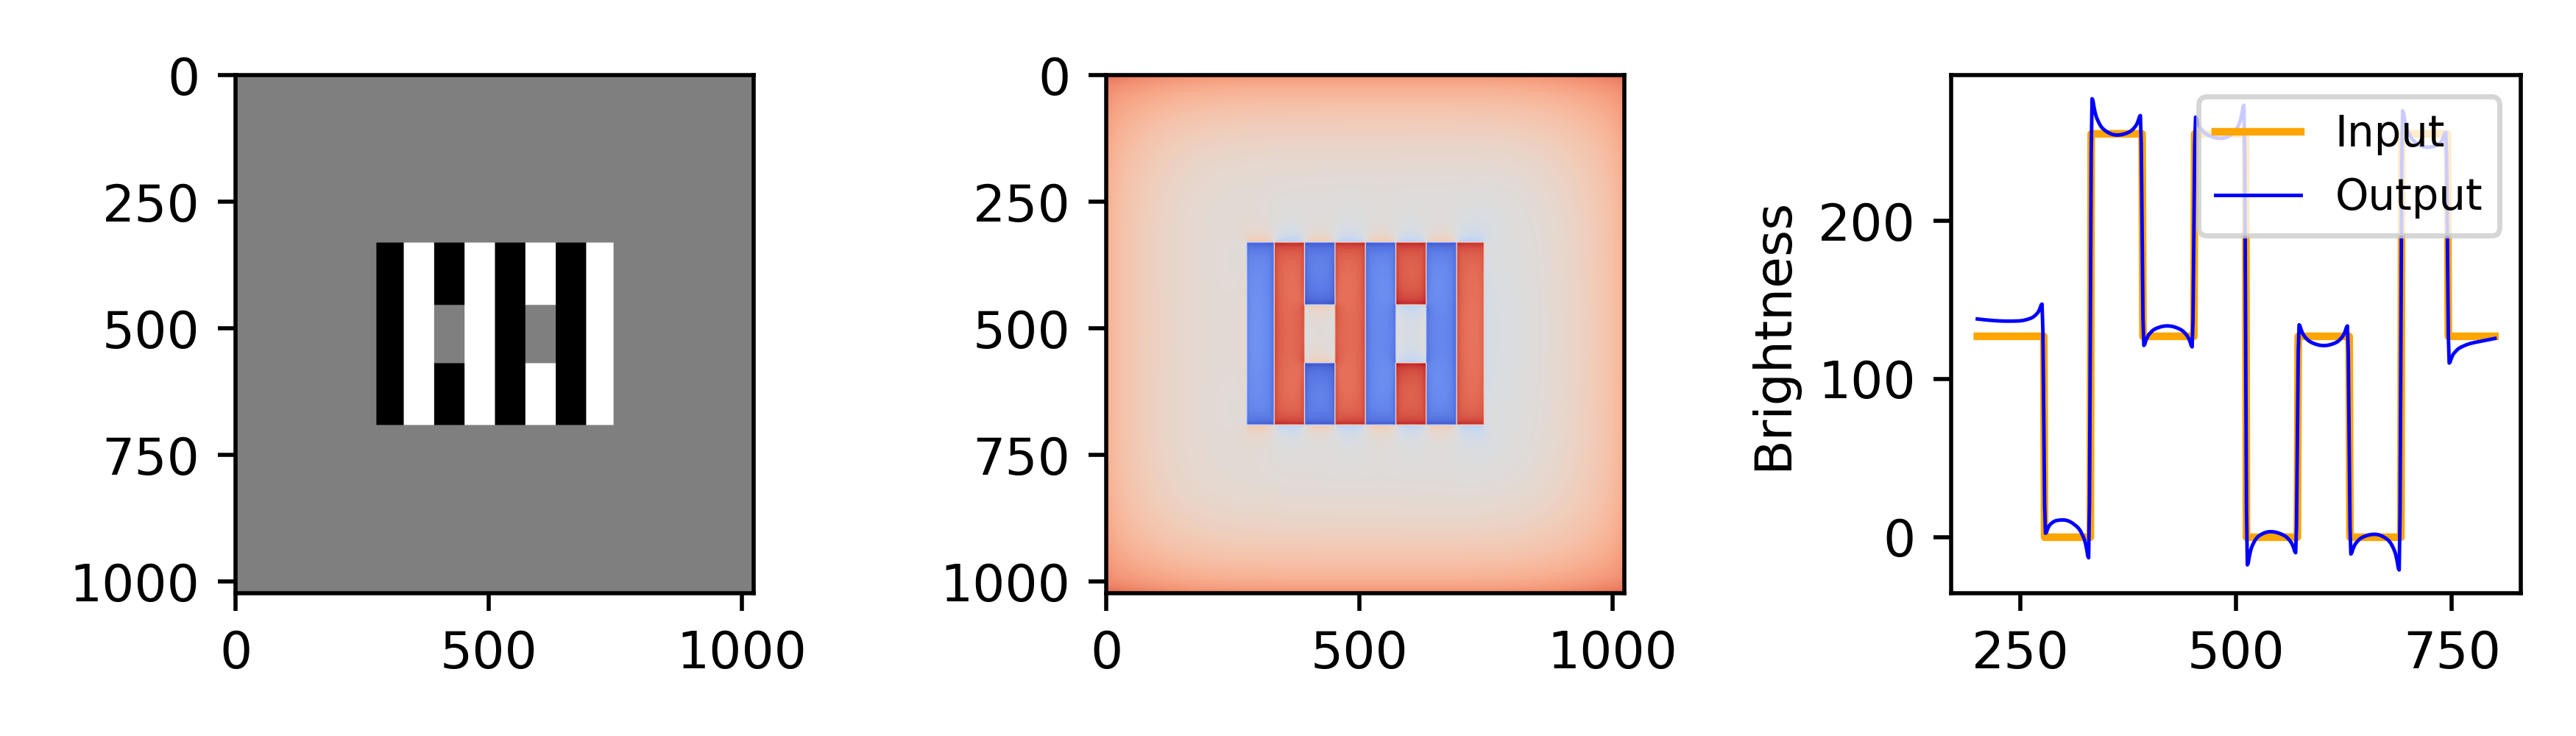
\includegraphics[width=\textwidth]{media/model_responses/odog_white_thick.png}
        \caption{Put your sub-caption here}
    \end{subfigure}
    \begin{subfigure}{0.8\textwidth}
        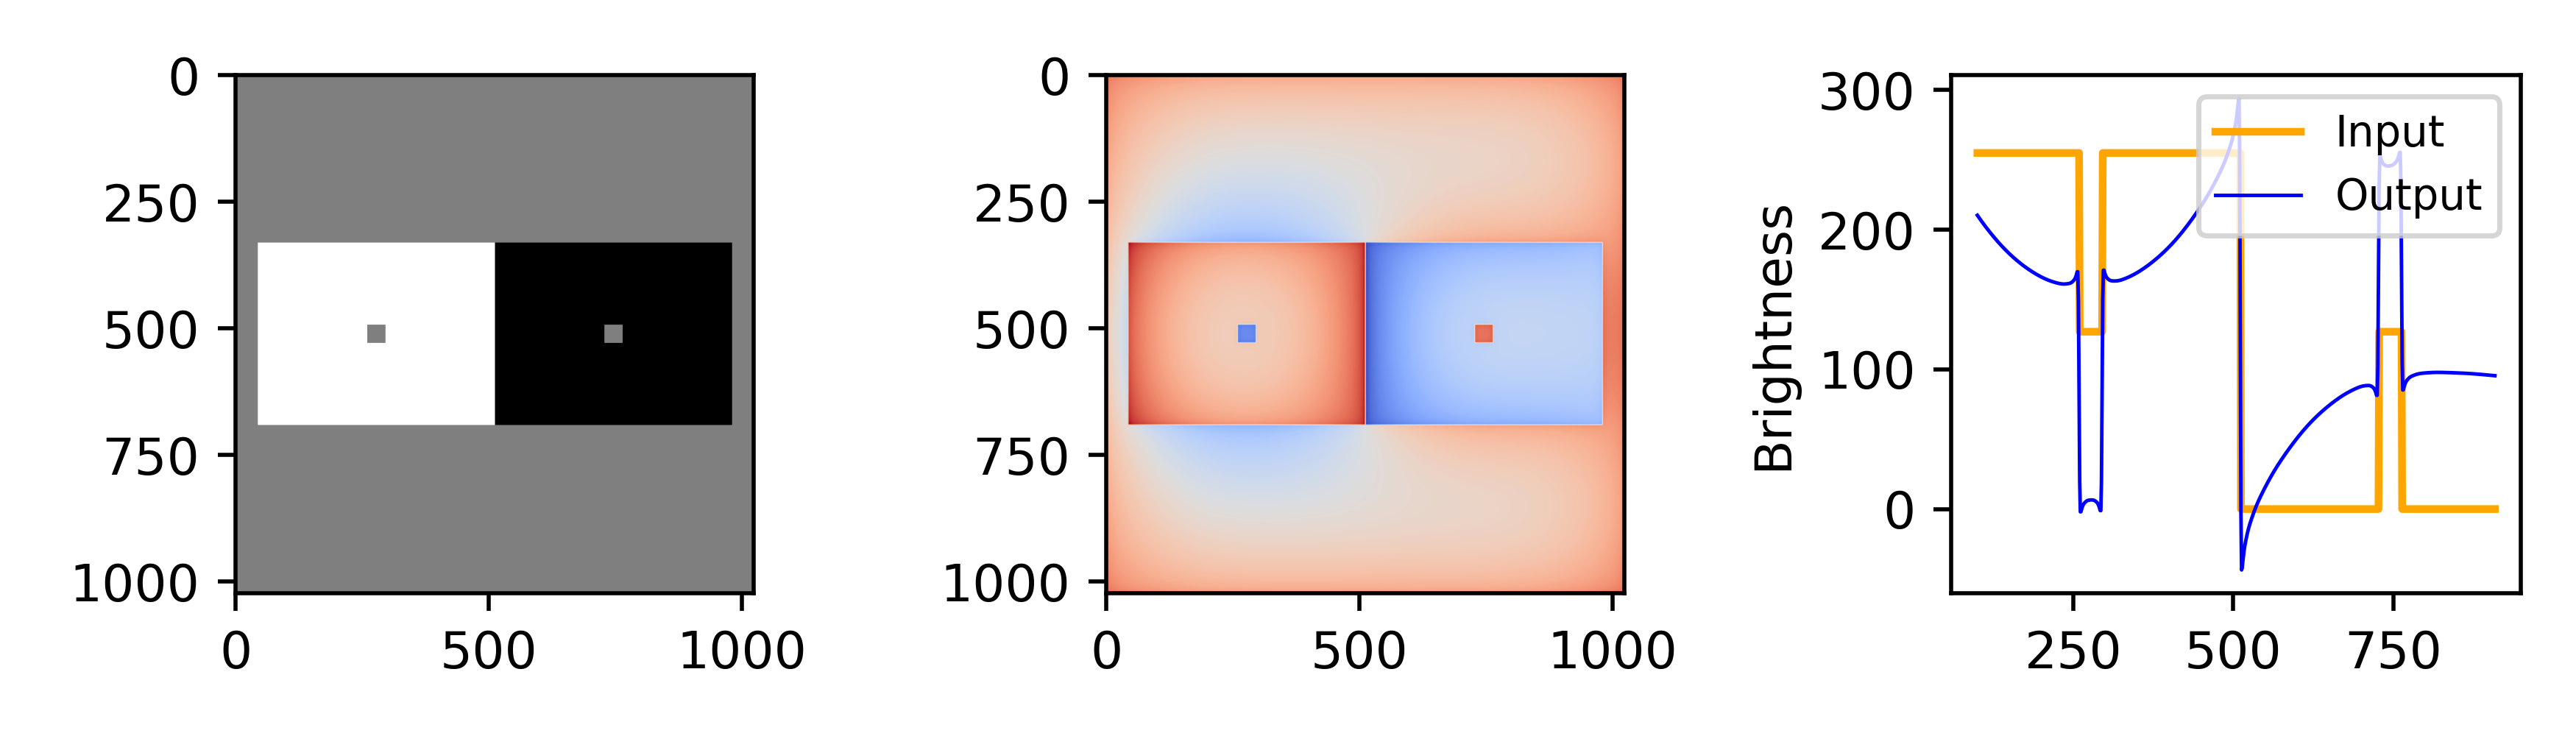
\includegraphics[width=\textwidth]{media/model_responses/odog_sbc_small.png}
        \caption{Put your sub-caption here}
    \end{subfigure}
    \begin{subfigure}{0.8\textwidth}
        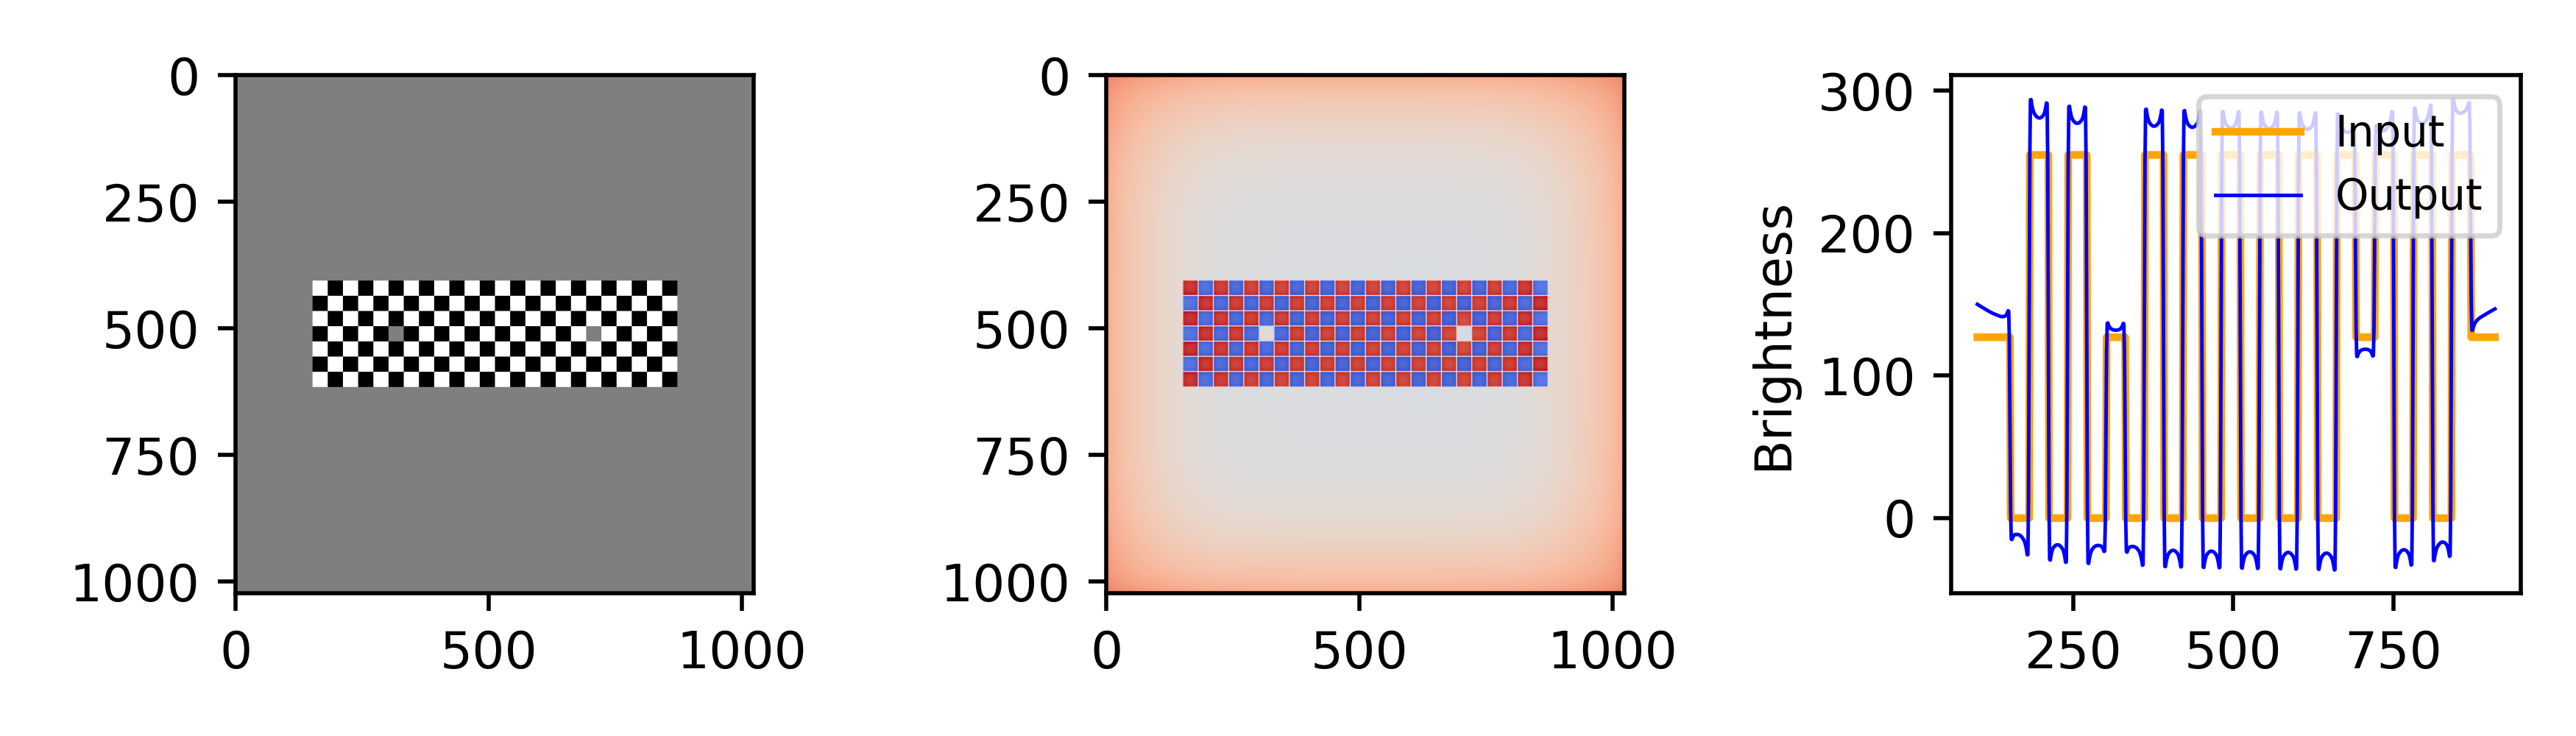
\includegraphics[width=\textwidth]{media/model_responses/odog_checkerboard.png}
        \caption{Put your sub-caption here}
    \end{subfigure}
    \begin{subfigure}{0.8\textwidth}
        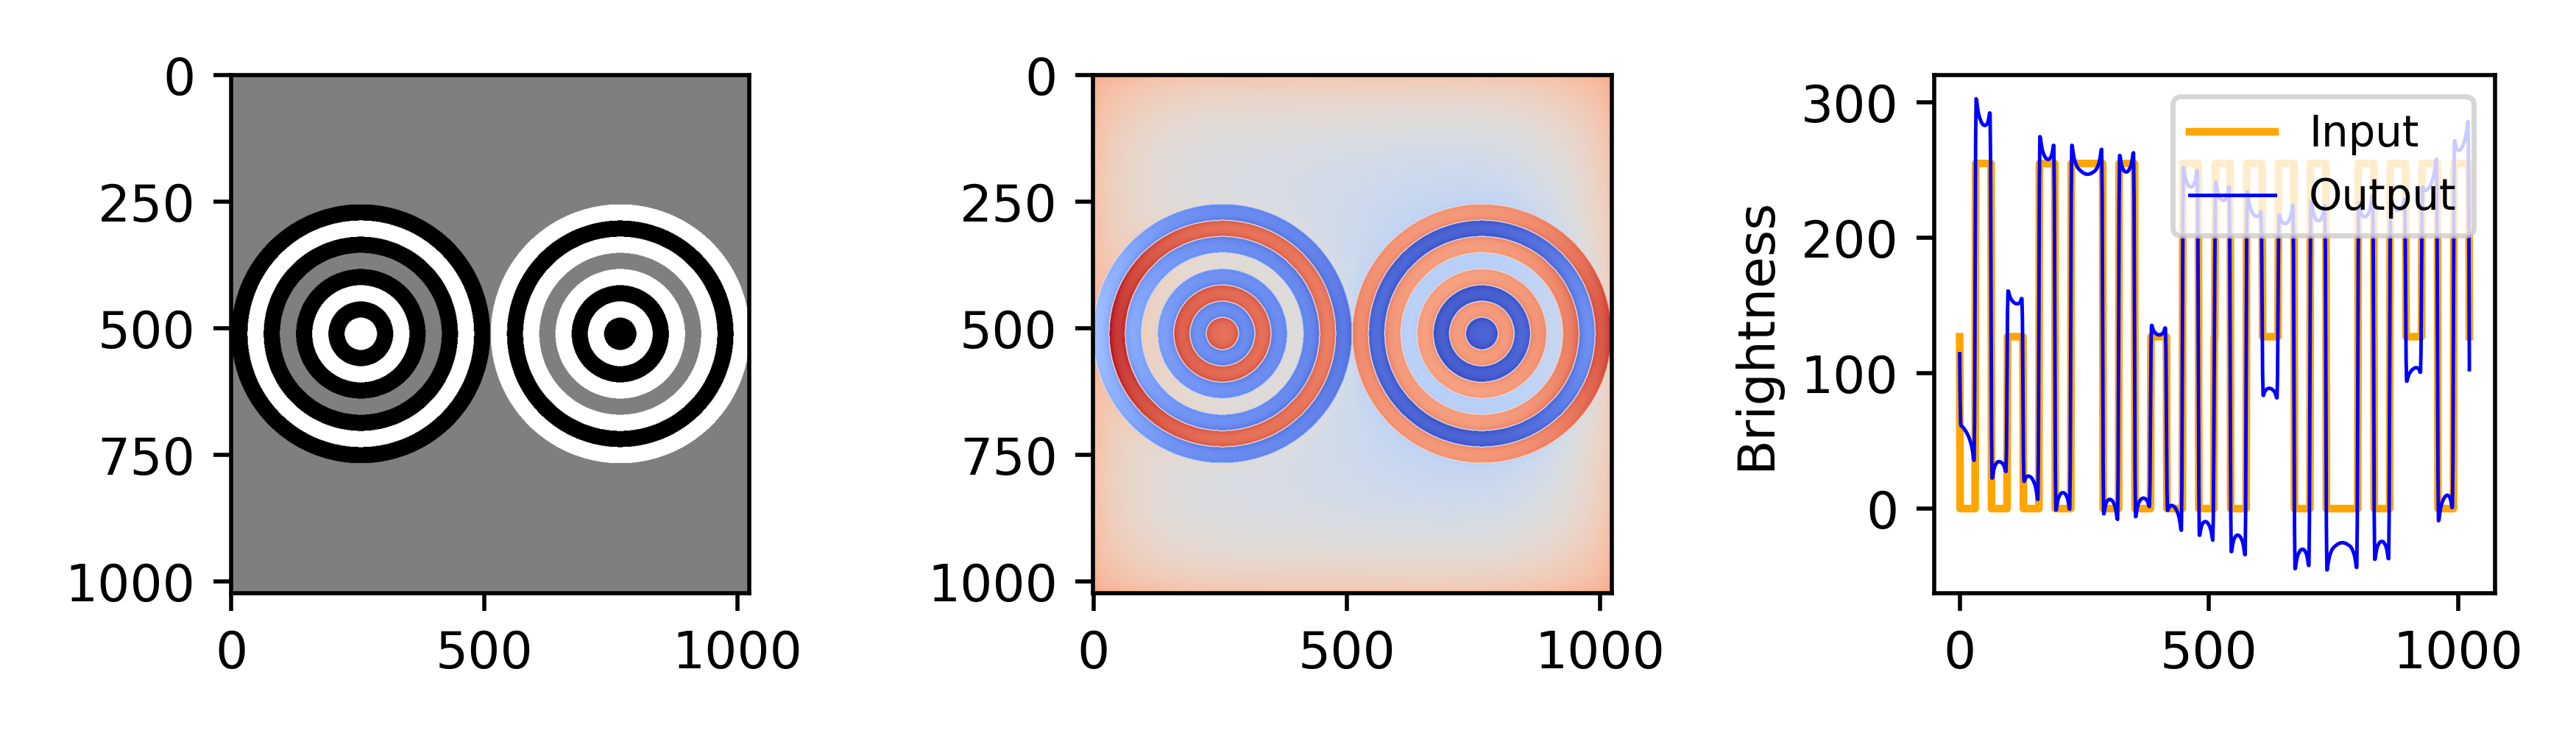
\includegraphics[width=\textwidth]{media/model_responses/odog_white_circular.png}
        \caption{Put your sub-caption here}
    \end{subfigure}
    \caption{Add your own figures before compiling}
    \label{fig:foobar}
\end{figure}

% \begin{figure}[H]
%     \centering
%     \begin{subfigure}{0.7\textwidth}
%         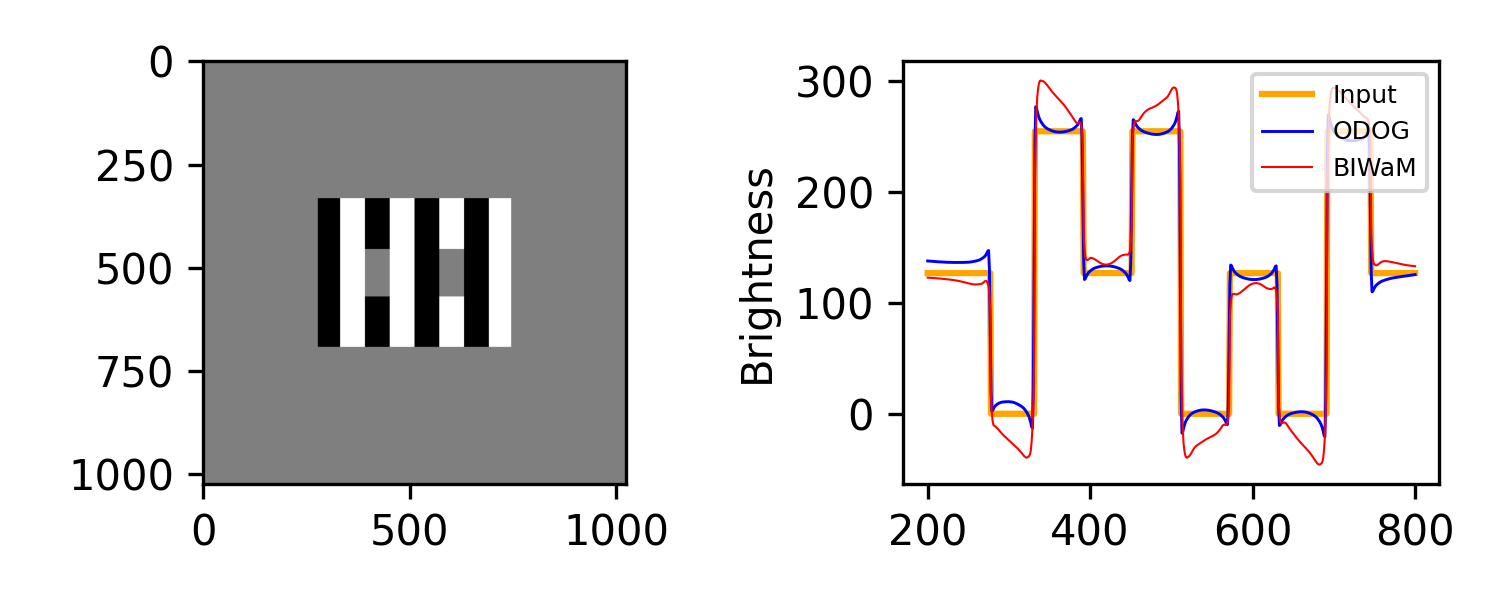
\includegraphics[width=\textwidth]{media/model_responses/both_white_thick.png}
%         \caption{Put your sub-caption here}
%     \end{subfigure}
%     \begin{subfigure}{0.7\textwidth}
%         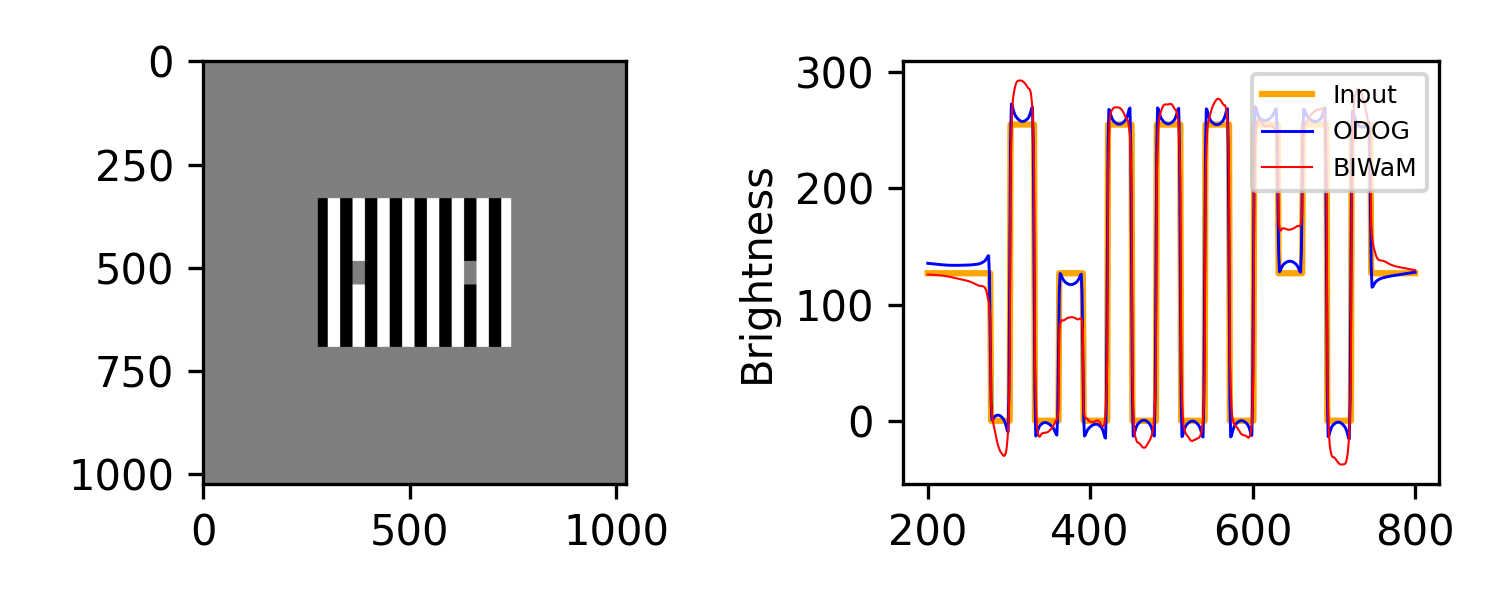
\includegraphics[width=\textwidth]{media/model_responses/both_white_thin.png}
%         \caption{Put your sub-caption here}
%     \end{subfigure}
%     \begin{subfigure}{0.7\textwidth}
%         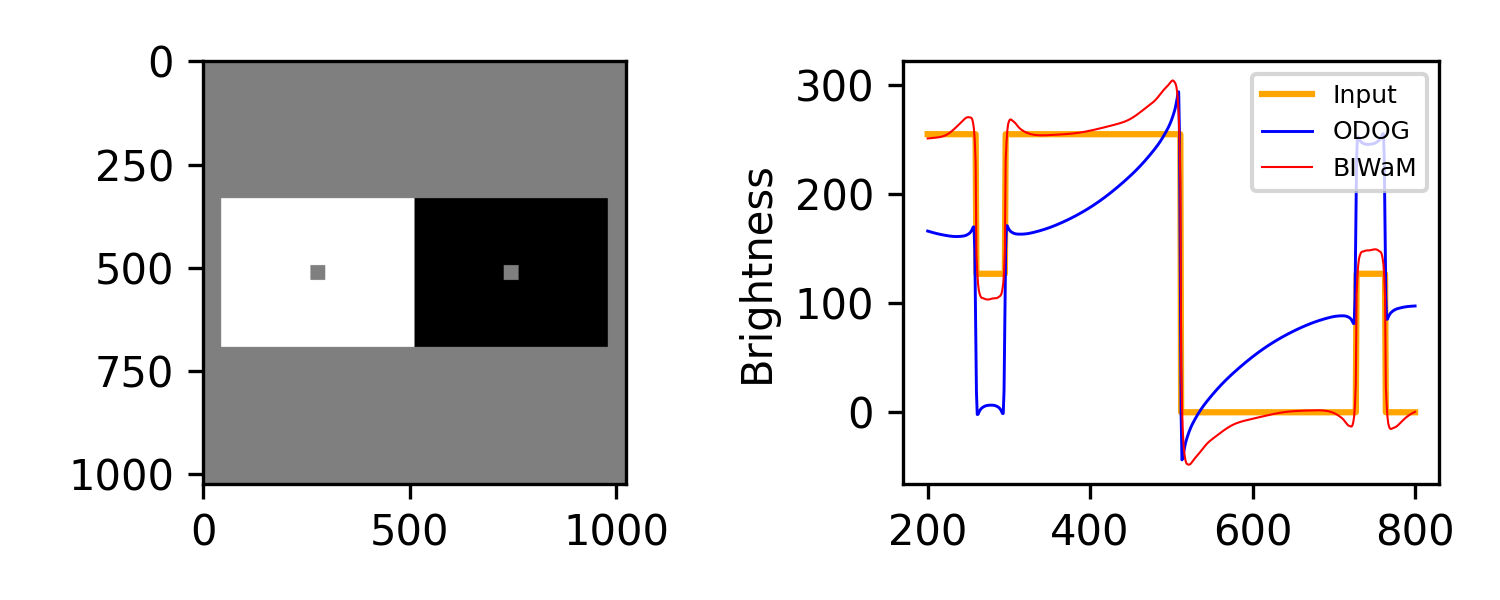
\includegraphics[width=\textwidth]{media/model_responses/both_sbc_small.png}
%         \caption{Put your sub-caption here}
%     \end{subfigure}
%     \begin{subfigure}{0.7\textwidth}
%         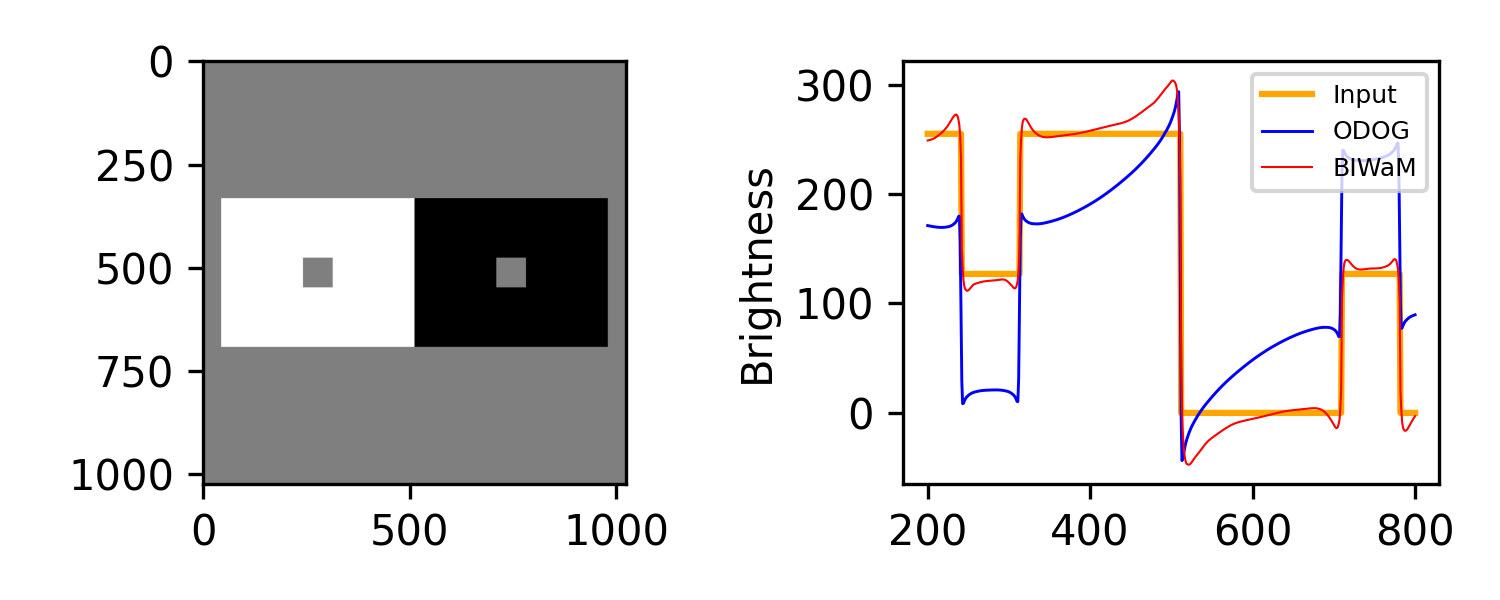
\includegraphics[width=\textwidth]{media/model_responses/both_sbc_large.png}
%         \caption{Put your sub-caption here}
%     \end{subfigure}
%     \caption{Add your own figures before compiling}
%     \label{fig:foobar}
% \end{figure}


\begin{figure}[H]
    \centering
    \begin{subfigure}{0.7\textwidth}
        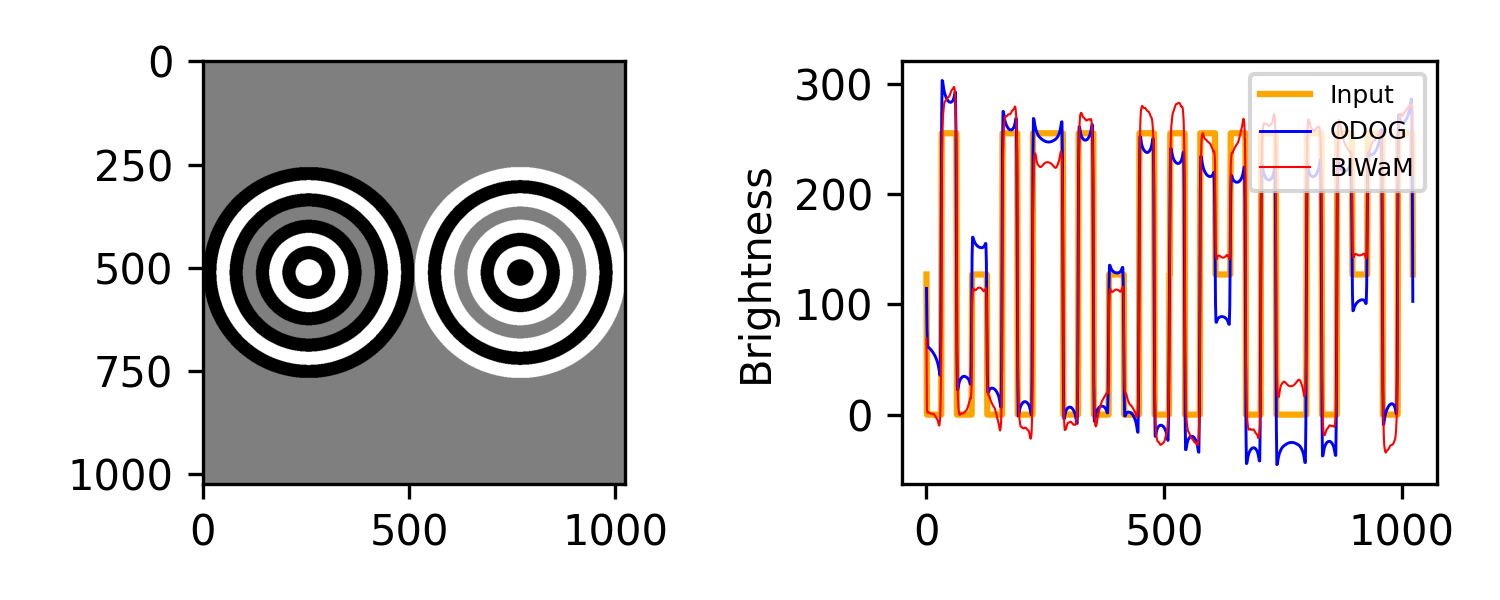
\includegraphics[width=\textwidth]{media/model_responses/both_white_circular.png}
        \caption{Put your sub-caption here}
    \end{subfigure}
    \begin{subfigure}{0.7\textwidth}
        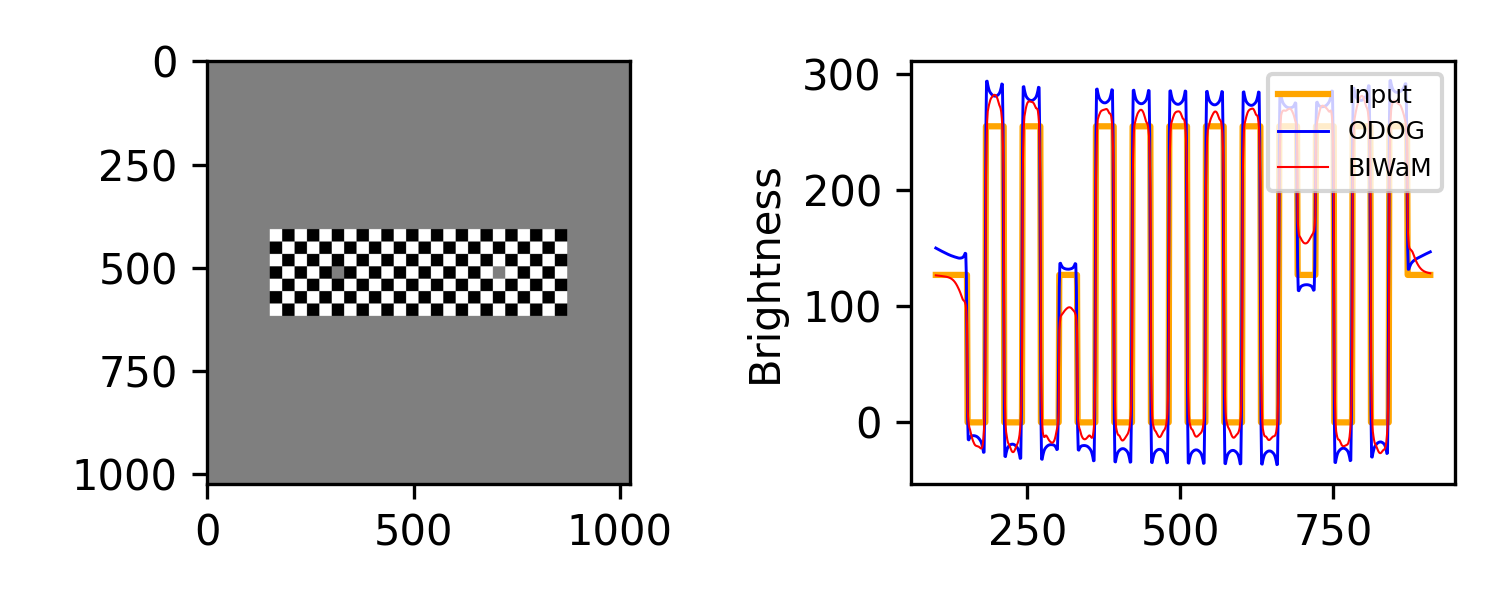
\includegraphics[width=\textwidth]{media/model_responses/both_checkerboard.png}
        \caption{Put your sub-caption here}
    \end{subfigure}
    \begin{subfigure}{0.7\textwidth}
        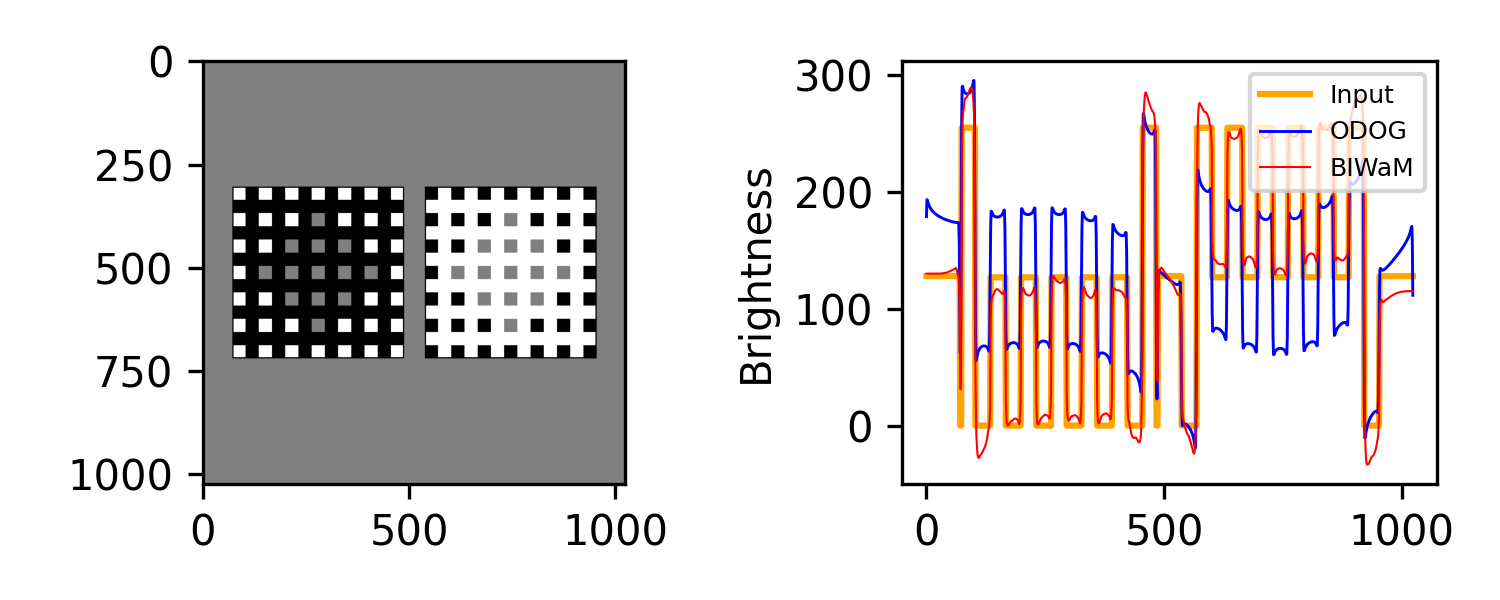
\includegraphics[width=\textwidth]{media/model_responses/both_dungeon.png}
        \caption{Put your sub-caption here}
    \end{subfigure}
\caption{Add your own figures before compiling}
    \label{fig:foobar}
\end{figure}


% \begin{figure}
%     \centering
%     \subfloat[fig 1]{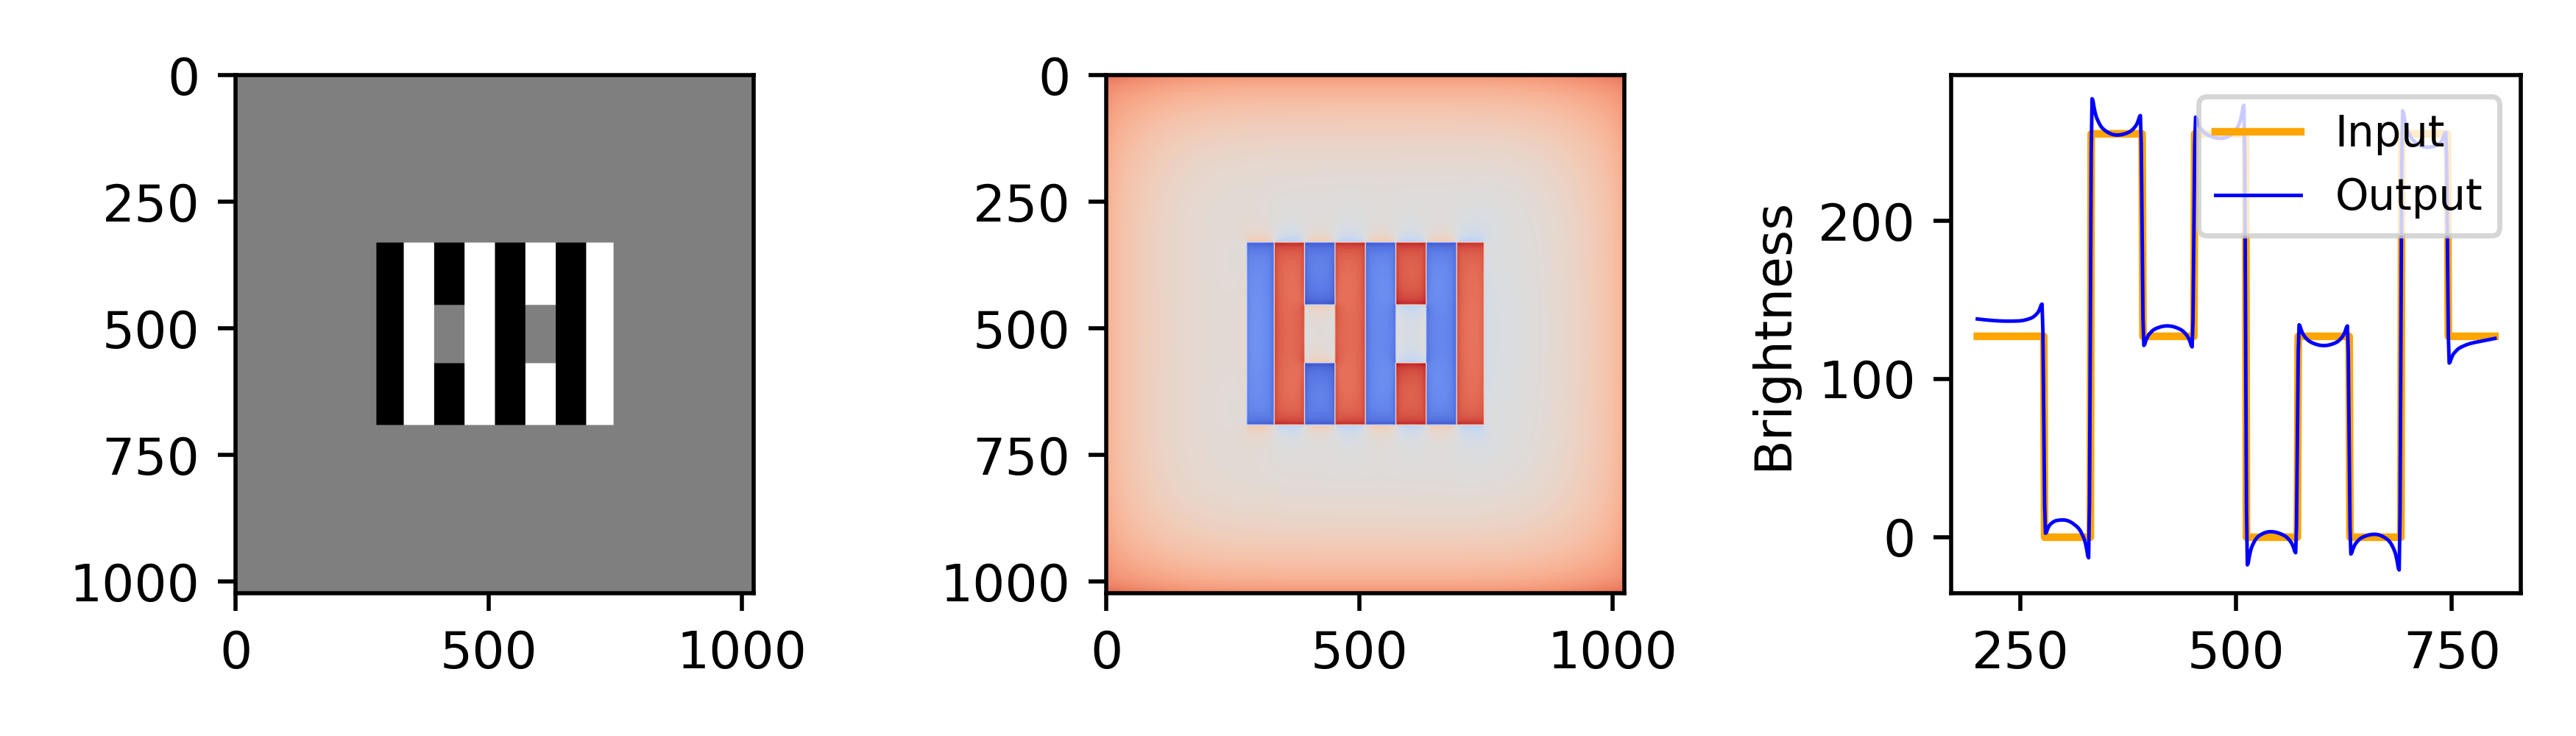
\includegraphics[width=\linewidth]{media/model_responses/odog_white_thick.png.png}}\\ 
%     \subfloat[fig 2]{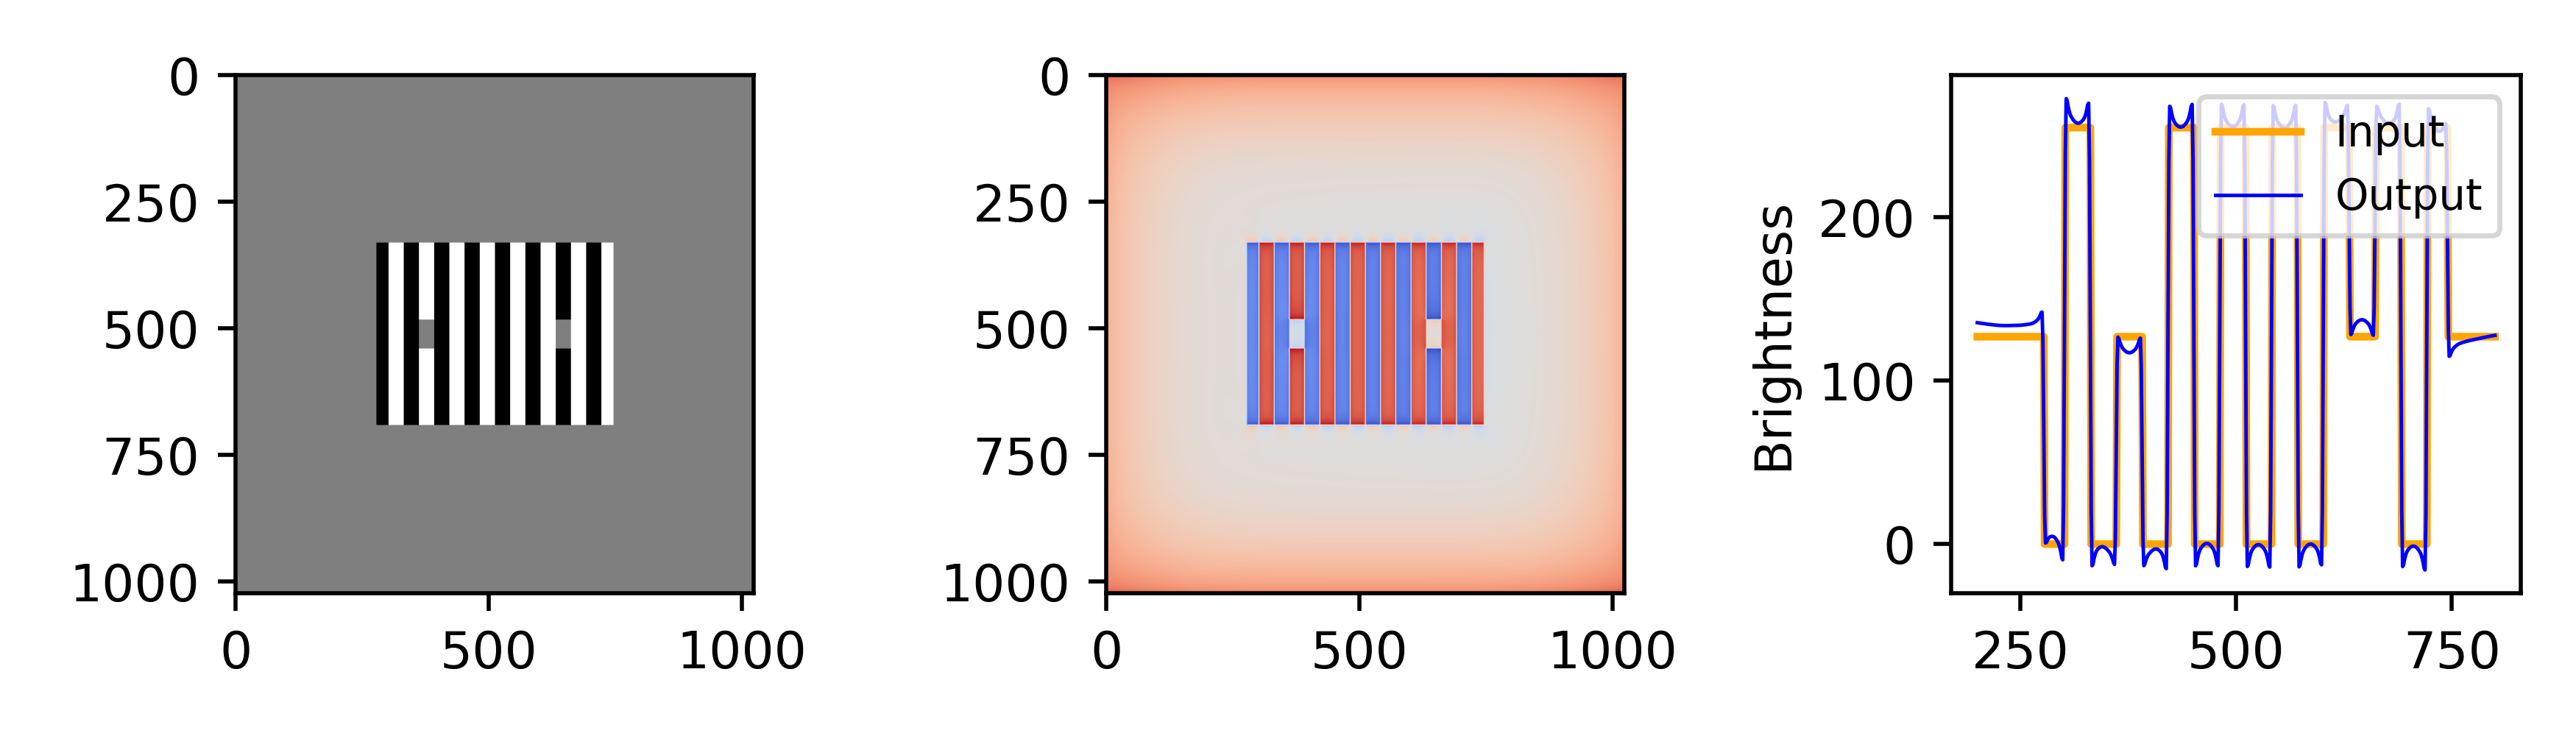
\includegraphics[width=\linewidth]{media/model_responses/odog_white_thin.png.png}}\\
%     \subfloat[fig 3]{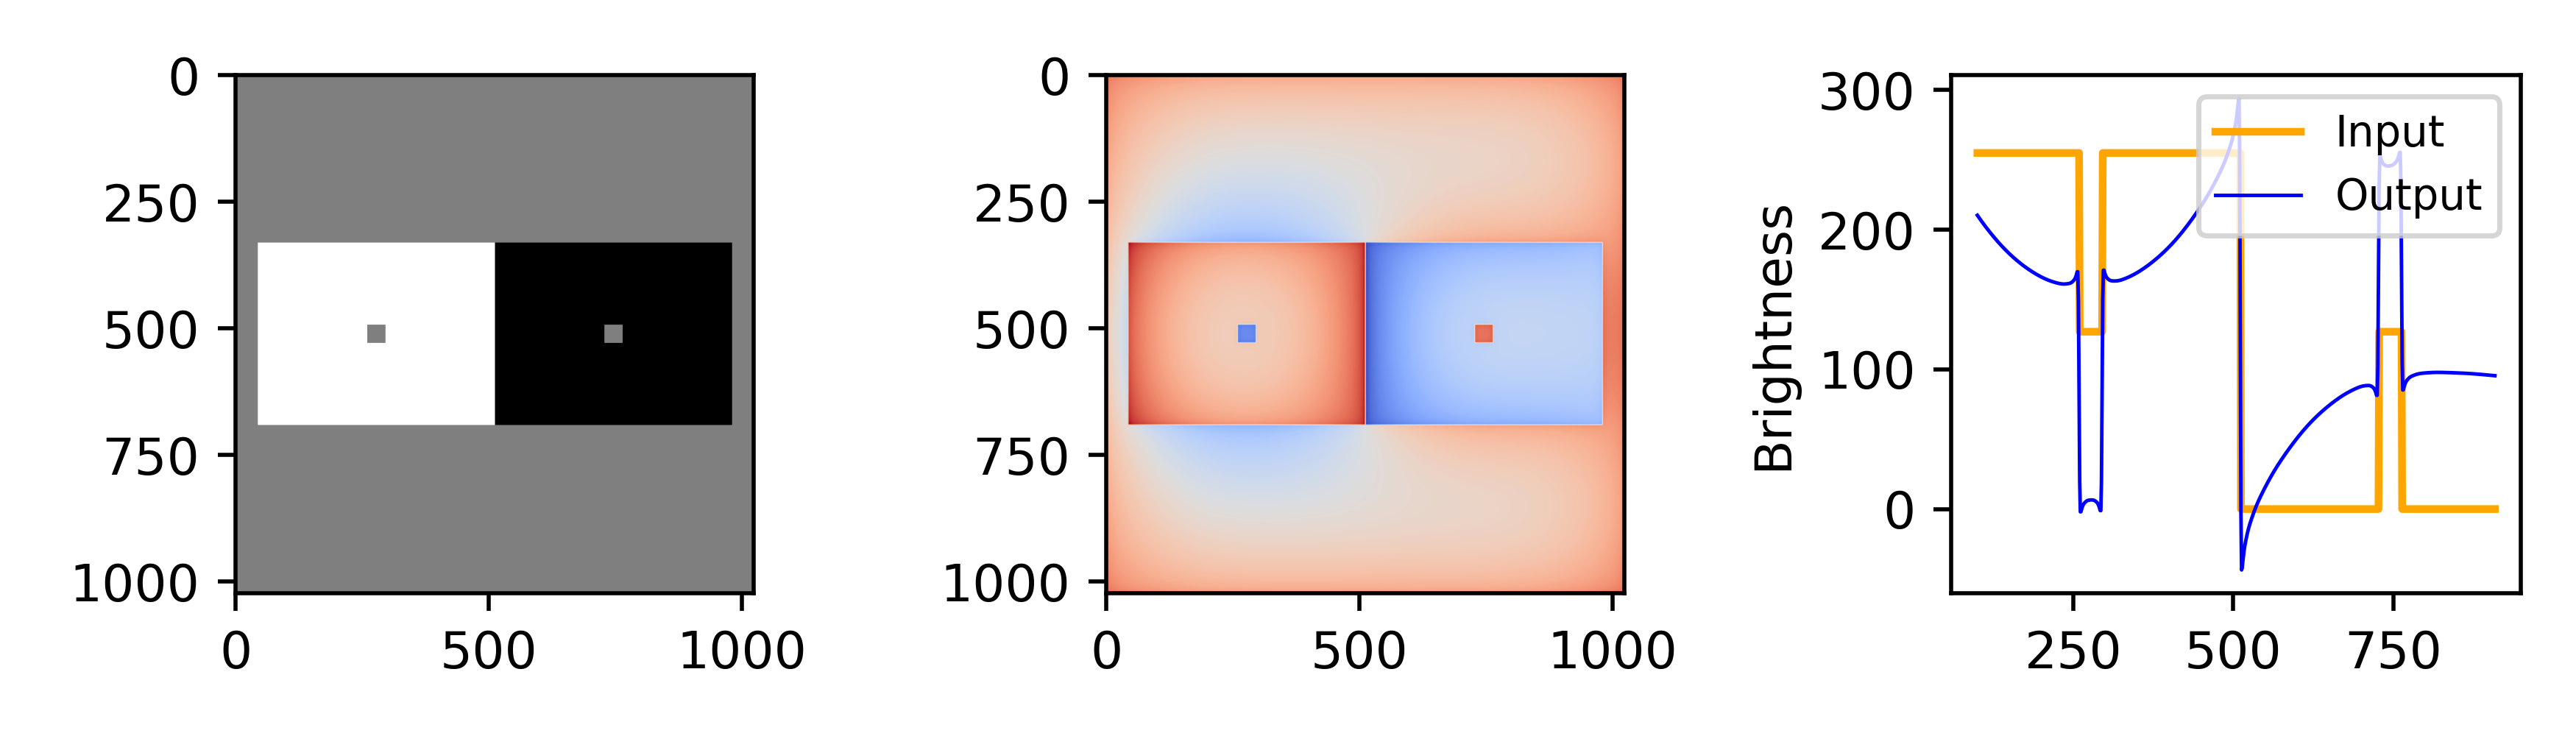
\includegraphics[width=\linewidth]{media/model_responses/odog_sbc_small.png.png}}\\
%     \subfloat[fig 4]{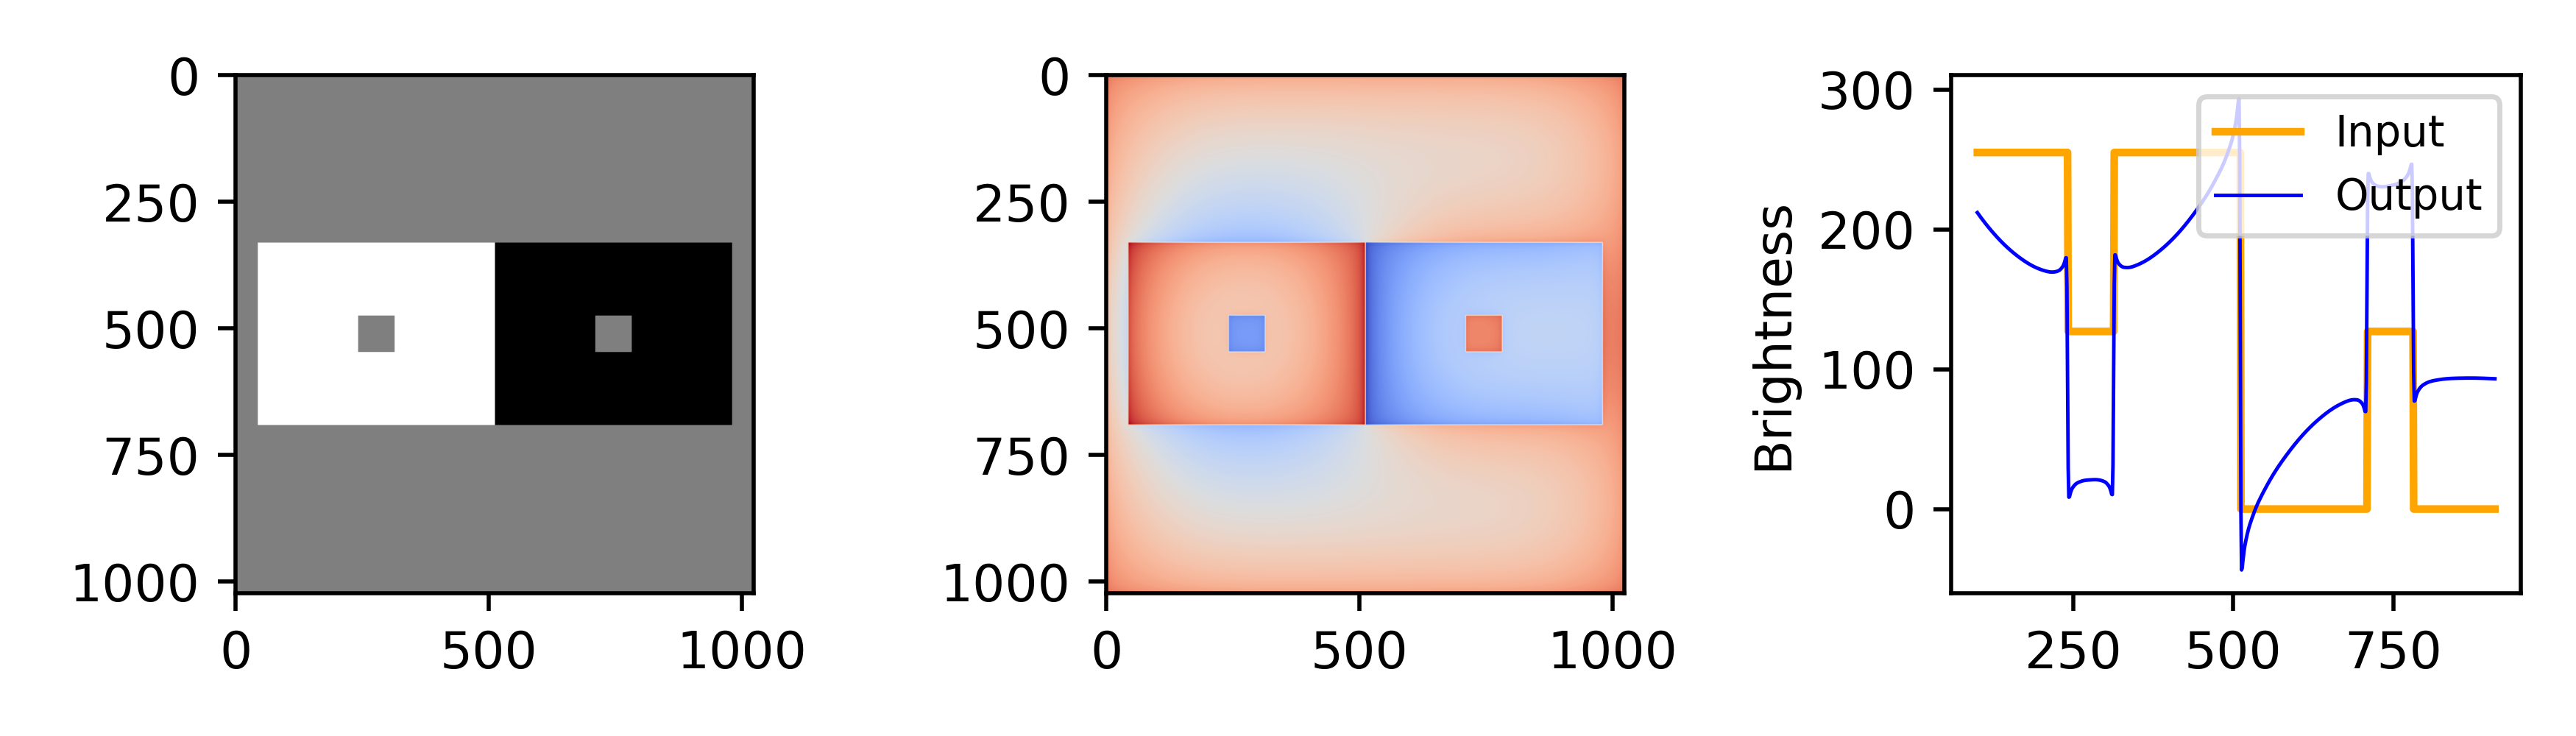
\includegraphics[width=\linewidth]{media/model_responses/odog_sbc_large.png.png}}\\
%     \caption{Add your own figures before compiling}
%     \label{some example}
% \end{figure}

% \begin{figure}
%     \centering
%     \subfloat[fig 5]{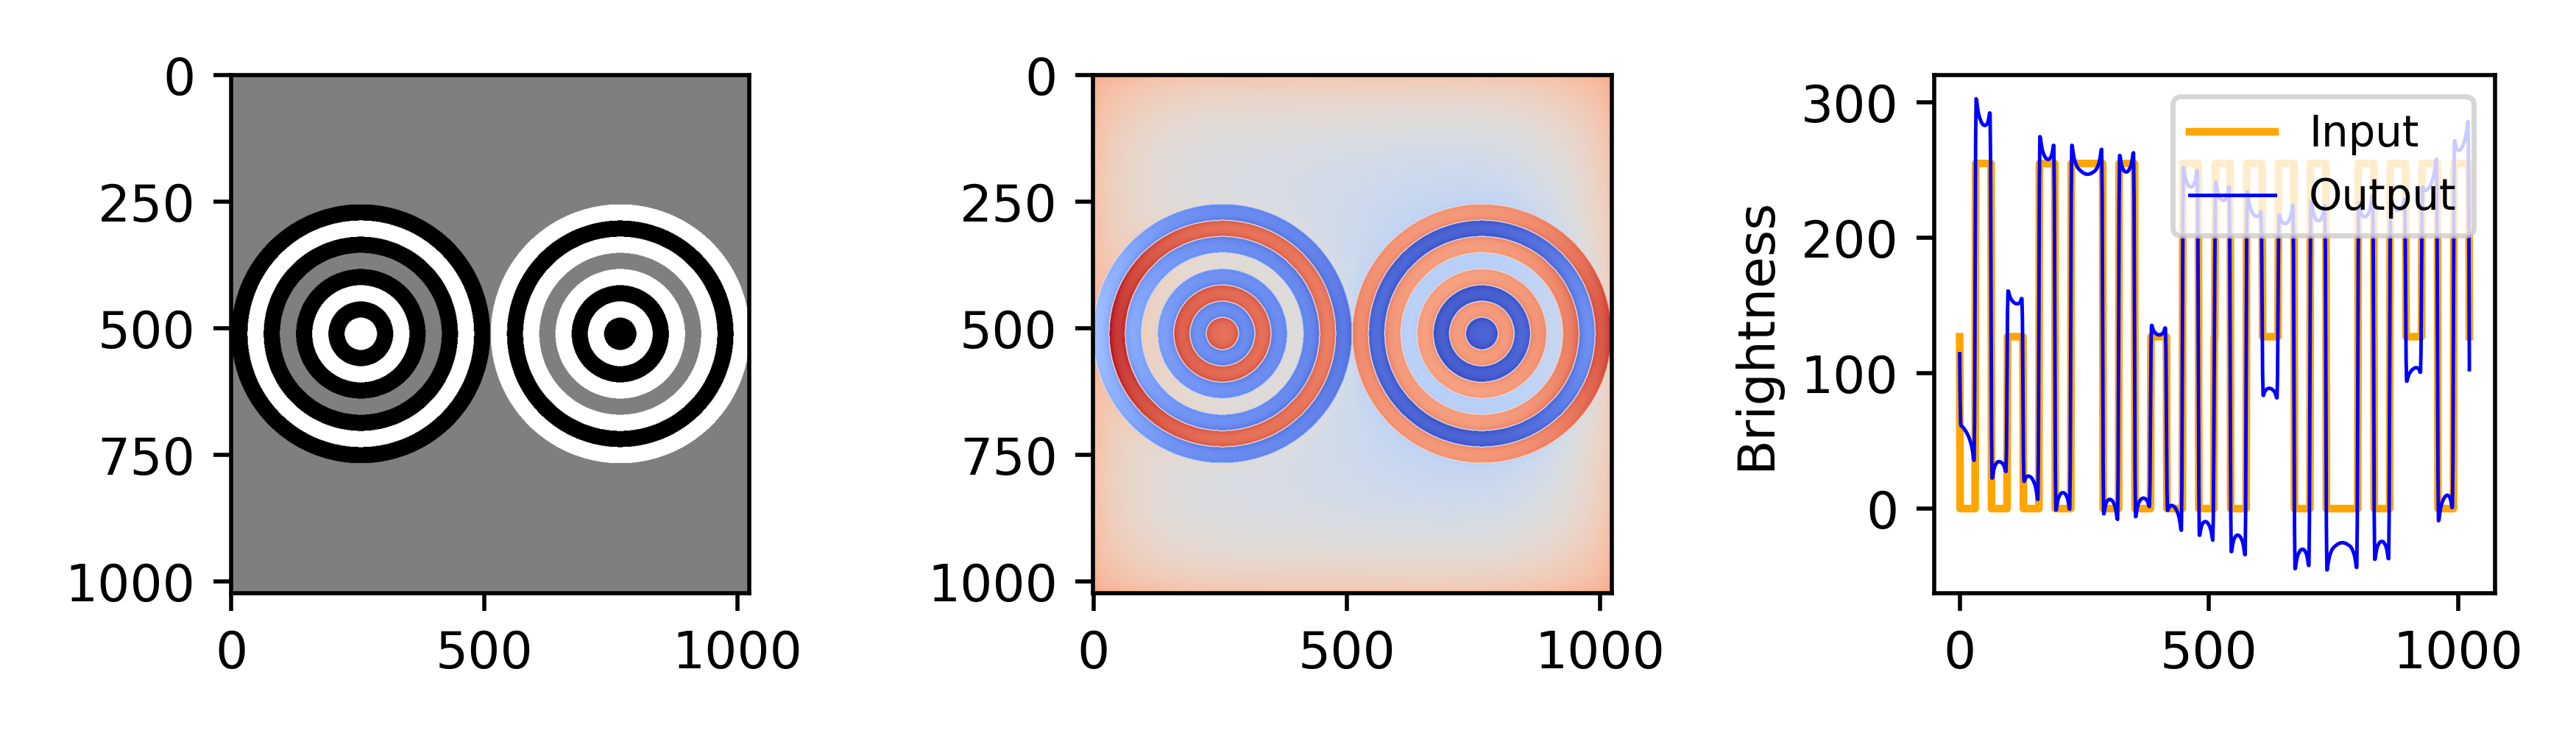
\includegraphics[width=\linewidth]{media/model_responses/odog_white_circular.png.png}}\\
%     \subfloat[fig 6]{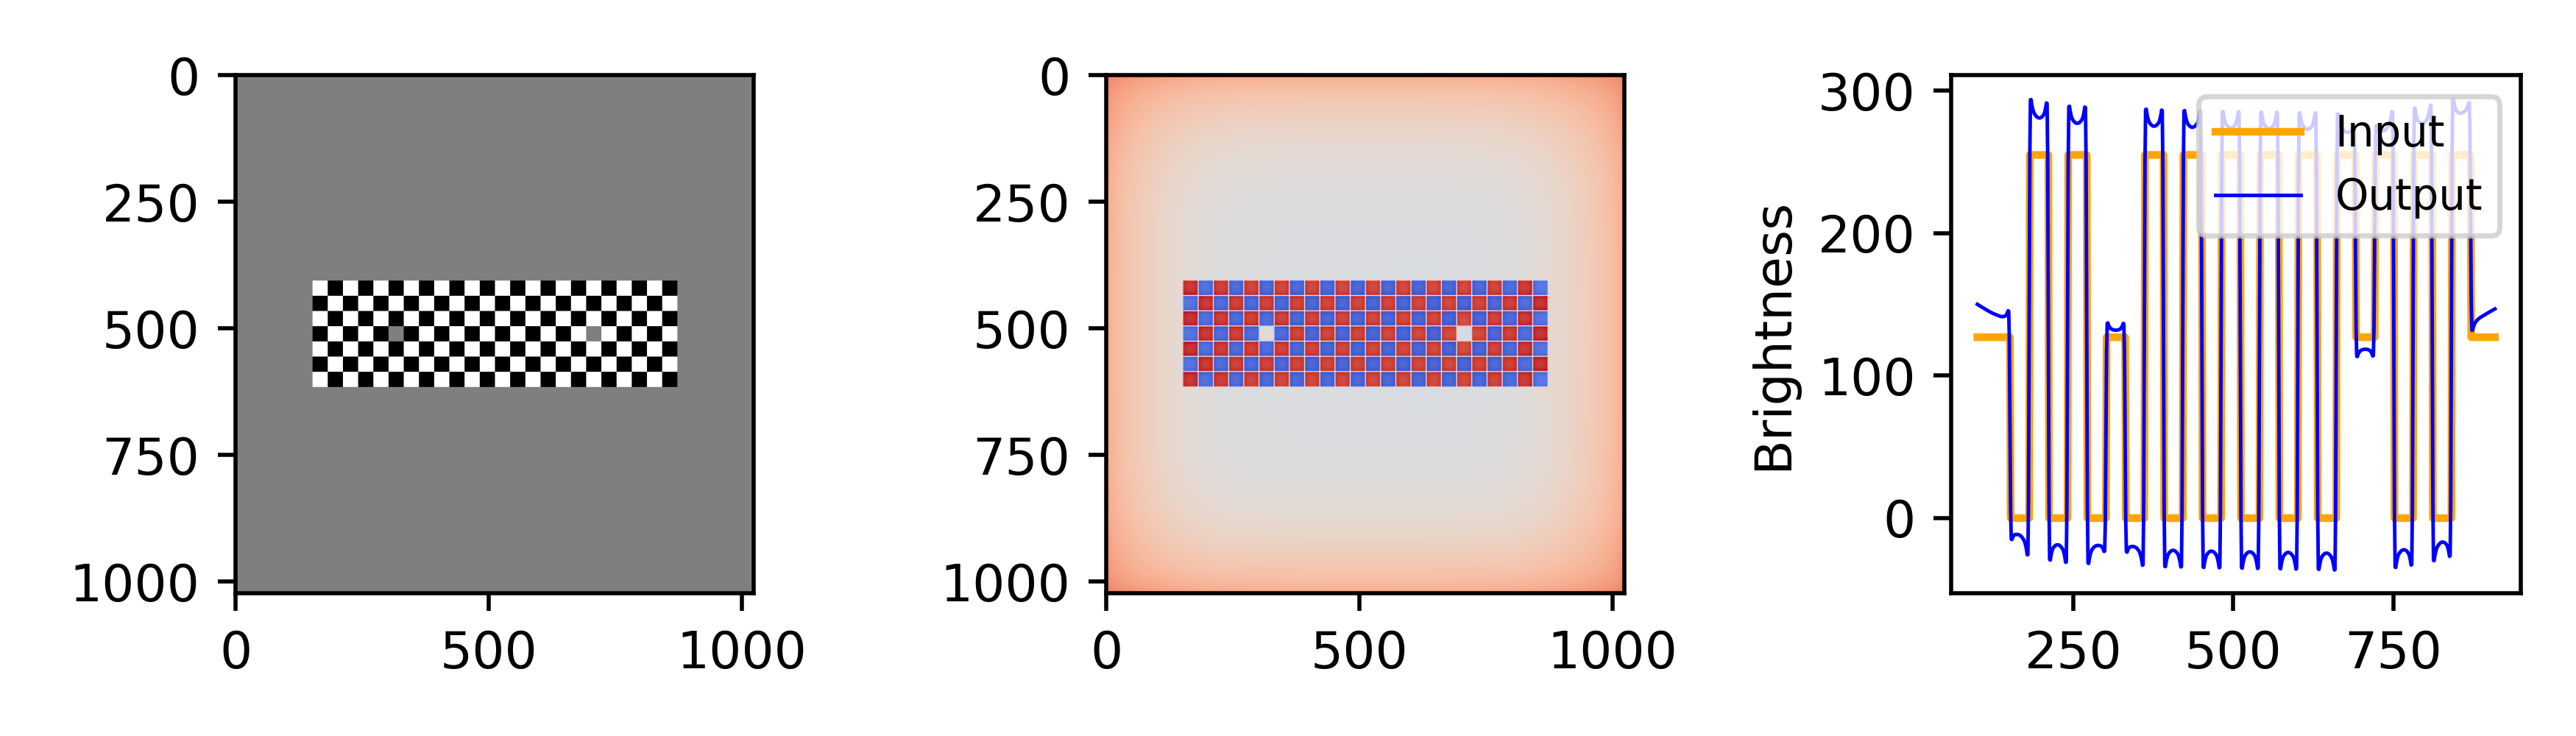
\includegraphics[width=\linewidth]{media/model_responses/odog_checkerboard.png.png}}\\ 
%     \subfloat[fig 7]{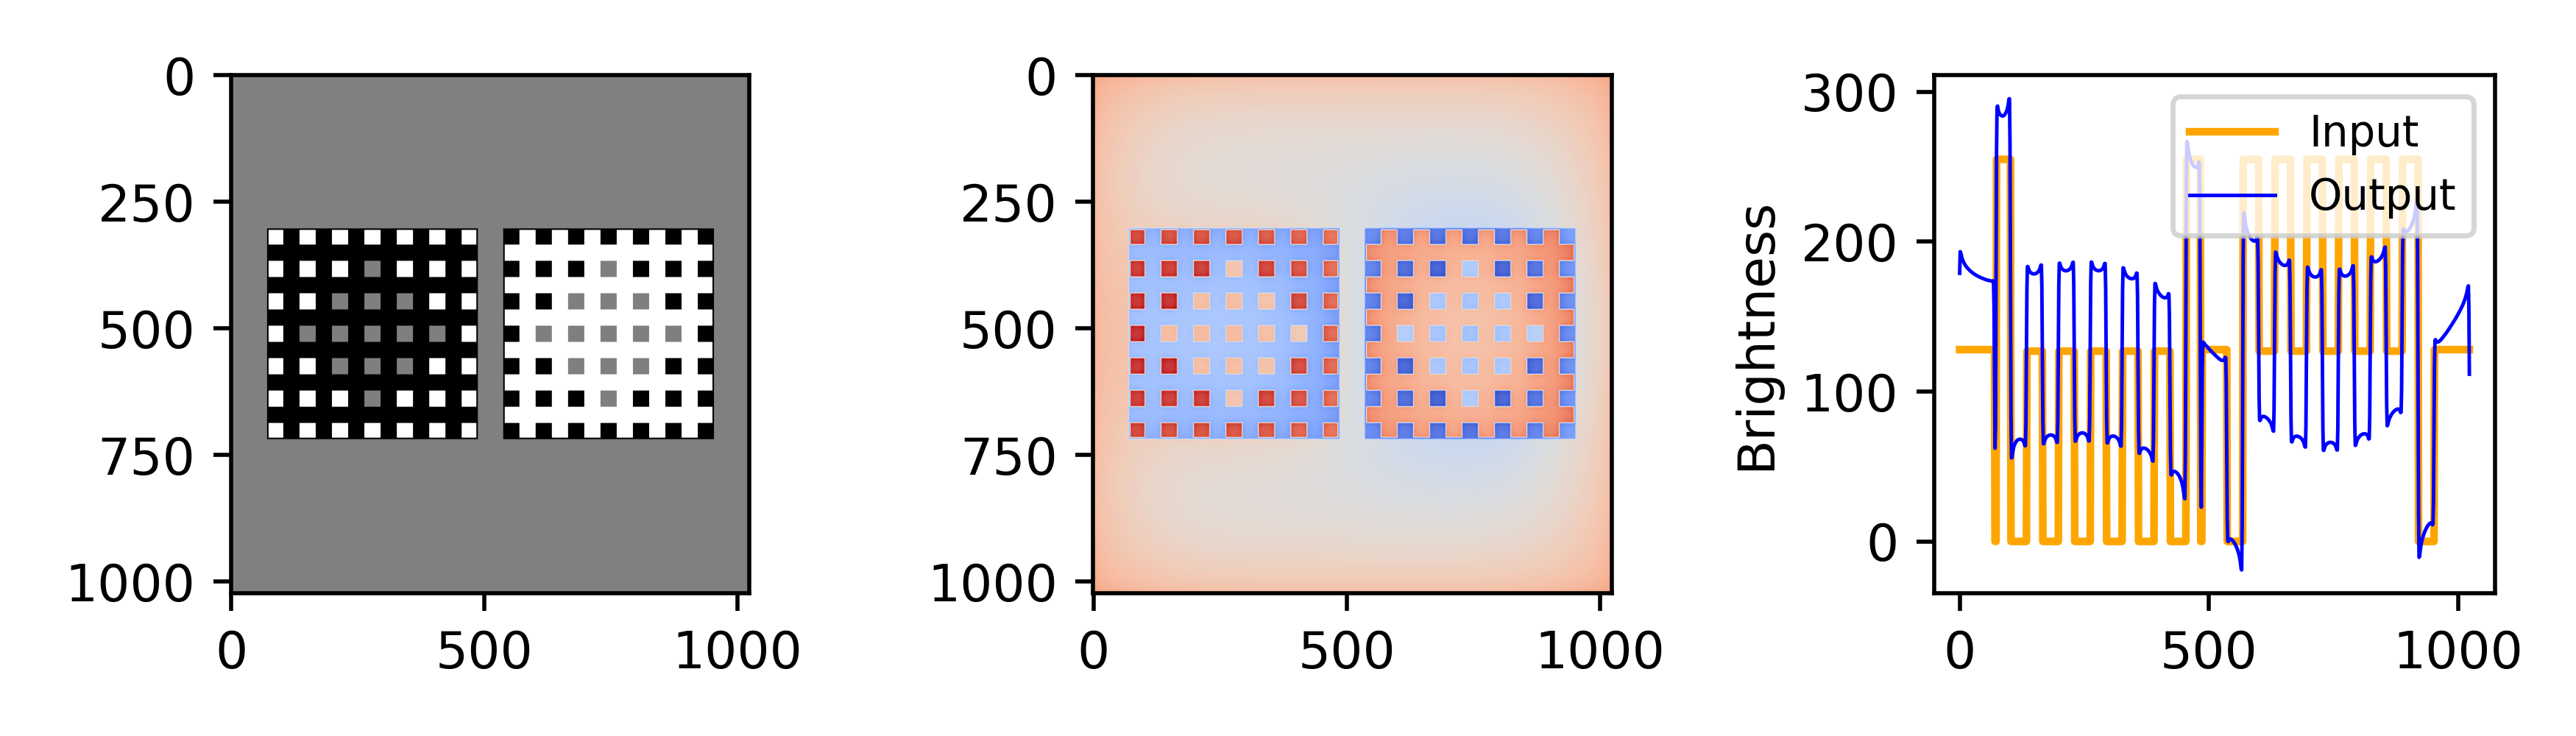
\includegraphics[width=\linewidth]{media/model_responses/odog_dungeon.png.png}}\\ 
%     \caption{Add your own figures before compiling}
%     \label{some example}
% \end{figure}

\textcolor{red}{Compare the model results across 7 stimuli: Where
do the models make different predictions?}


\subsection{Preparations and Tools}
\textcolor{red}{TODO: write out the bullet points}
\begin{itemize}
    \item To modify the models, it was necessary to have access to their source codes
    \item for ODOG i used the Multyscale library (version 0.2)
    \item for BIWaM i used a python reimplementation of the available Matlab code (which
    is tested to work the same, see appendix)
    \item I recreated the input stimuli using the Stimupy package (version 1.1.2).
    \item For the thesis i used Python 3.12.7,  Jupyter Client 8.6.2, Matplotlib 3.9.1,
    Numpy 2.1.3, Scipy 1.14.0
\end{itemize}



\newpage
%_/_/_/_/_/_/_/_/_/_/_/_/_/_/_/_/_/_/_/_/_/_/_/_/_/_/_/_/_/_/
\section{Robustness}

\begin{figure}[H]
    \centering
    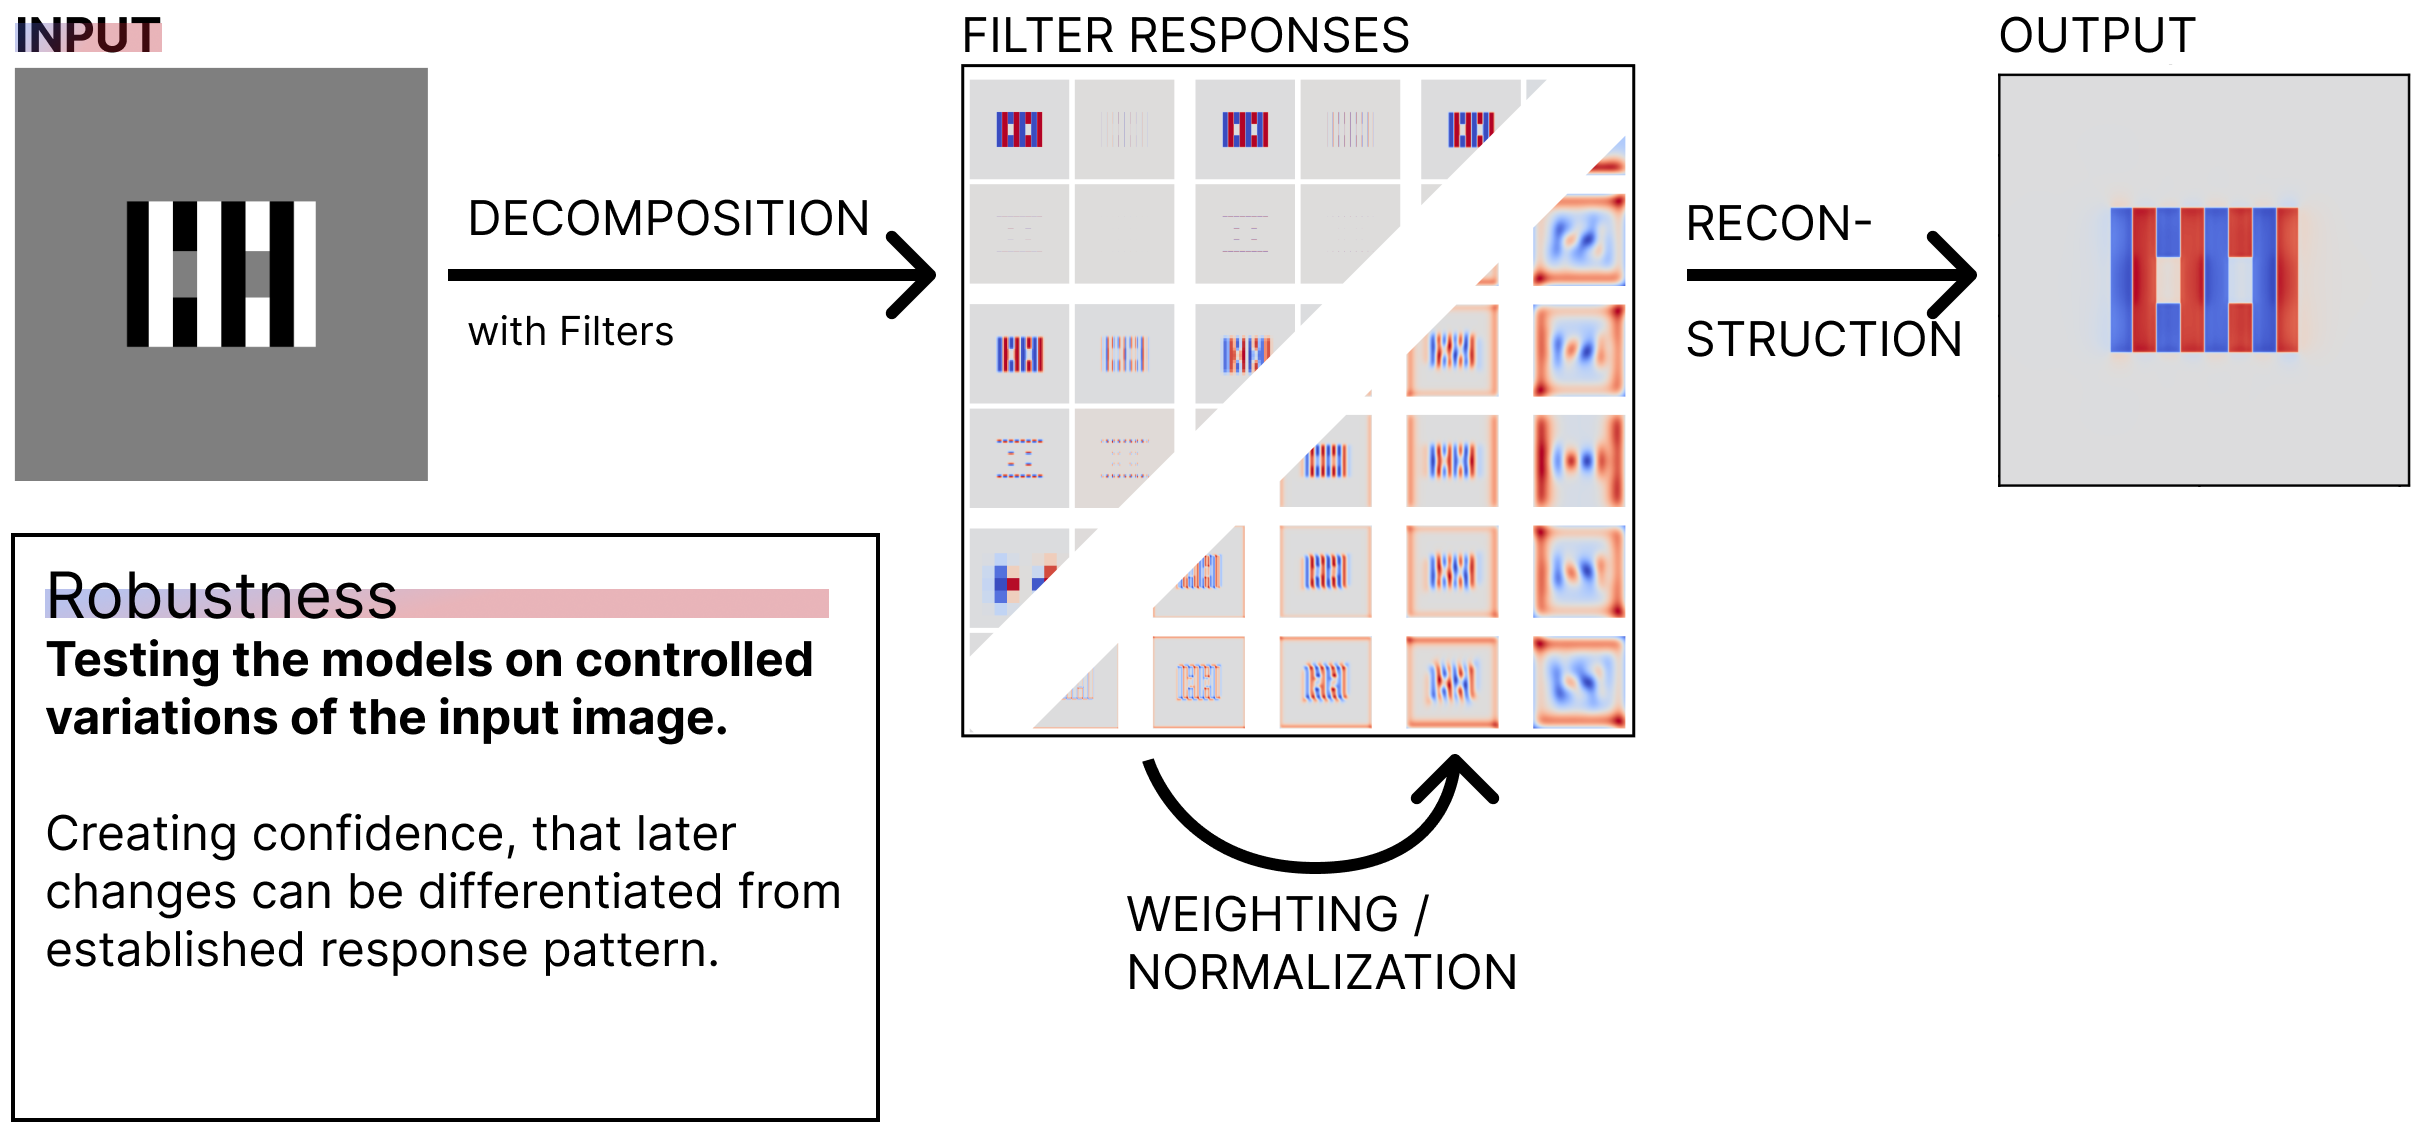
\includegraphics[width=\linewidth]{media/methodology/robustness_overview.png}
    \begin{minipage}{0.8\textwidth}
    \caption{Methodology overview of robustness testing}
    \label{fig:figure10}
    \end{minipage}
\end{figure}
In the Methodology section \textcolor{red}{referece} a baseline condition was established,
where the results reflected the interplay between the specific stimulus and the model with
its set parameters. Here, I aimed to determine whether this baseline condition is specific
to the exact interplay of these factors or if it can be generalized. Before changing
parameters in the next chapters, I want to ensure that the patterns of the model responses
on the stimuli are robust and can serve as a reliable comparison point.

To evaluate robustness, I applied both ODOG and BIWaM to a set of test stimuli that
underwent controlled, reasonably modifications. These modifications included: Brightness of
target patches, brightness of background, size of image content, size of target patches.

By observing the output patterns under these controlled changes, I aimed to answer two key
questions: 
\begin{itemize}
    \item What are the overall patterns of the models for the 7 test stimuli?
    \item Does the output changes in predictable ways?
\end{itemize}

\textcolor{red}{TODO: go through robustness tests, explain what i did, show the plots and
point out the predictable behavior.}

The robustness observed in both models provides a solid foundation for parameter tuning.
Since the outputs are predictable and generalizable under reasonably changes to the input
images, I am confident that future changes in the response pattern compared to the tested
baseline can be meaningfully attributed to parameter adjustments.

\newpage
%_/_/_/_/_/_/_/_/_/_/_/_/_/_/_/_/_/_/_/_/_/_/_/_/_/_/_/_/_/_/
\section{Decomposition parameters}

\begin{figure}[H]
    \centering
    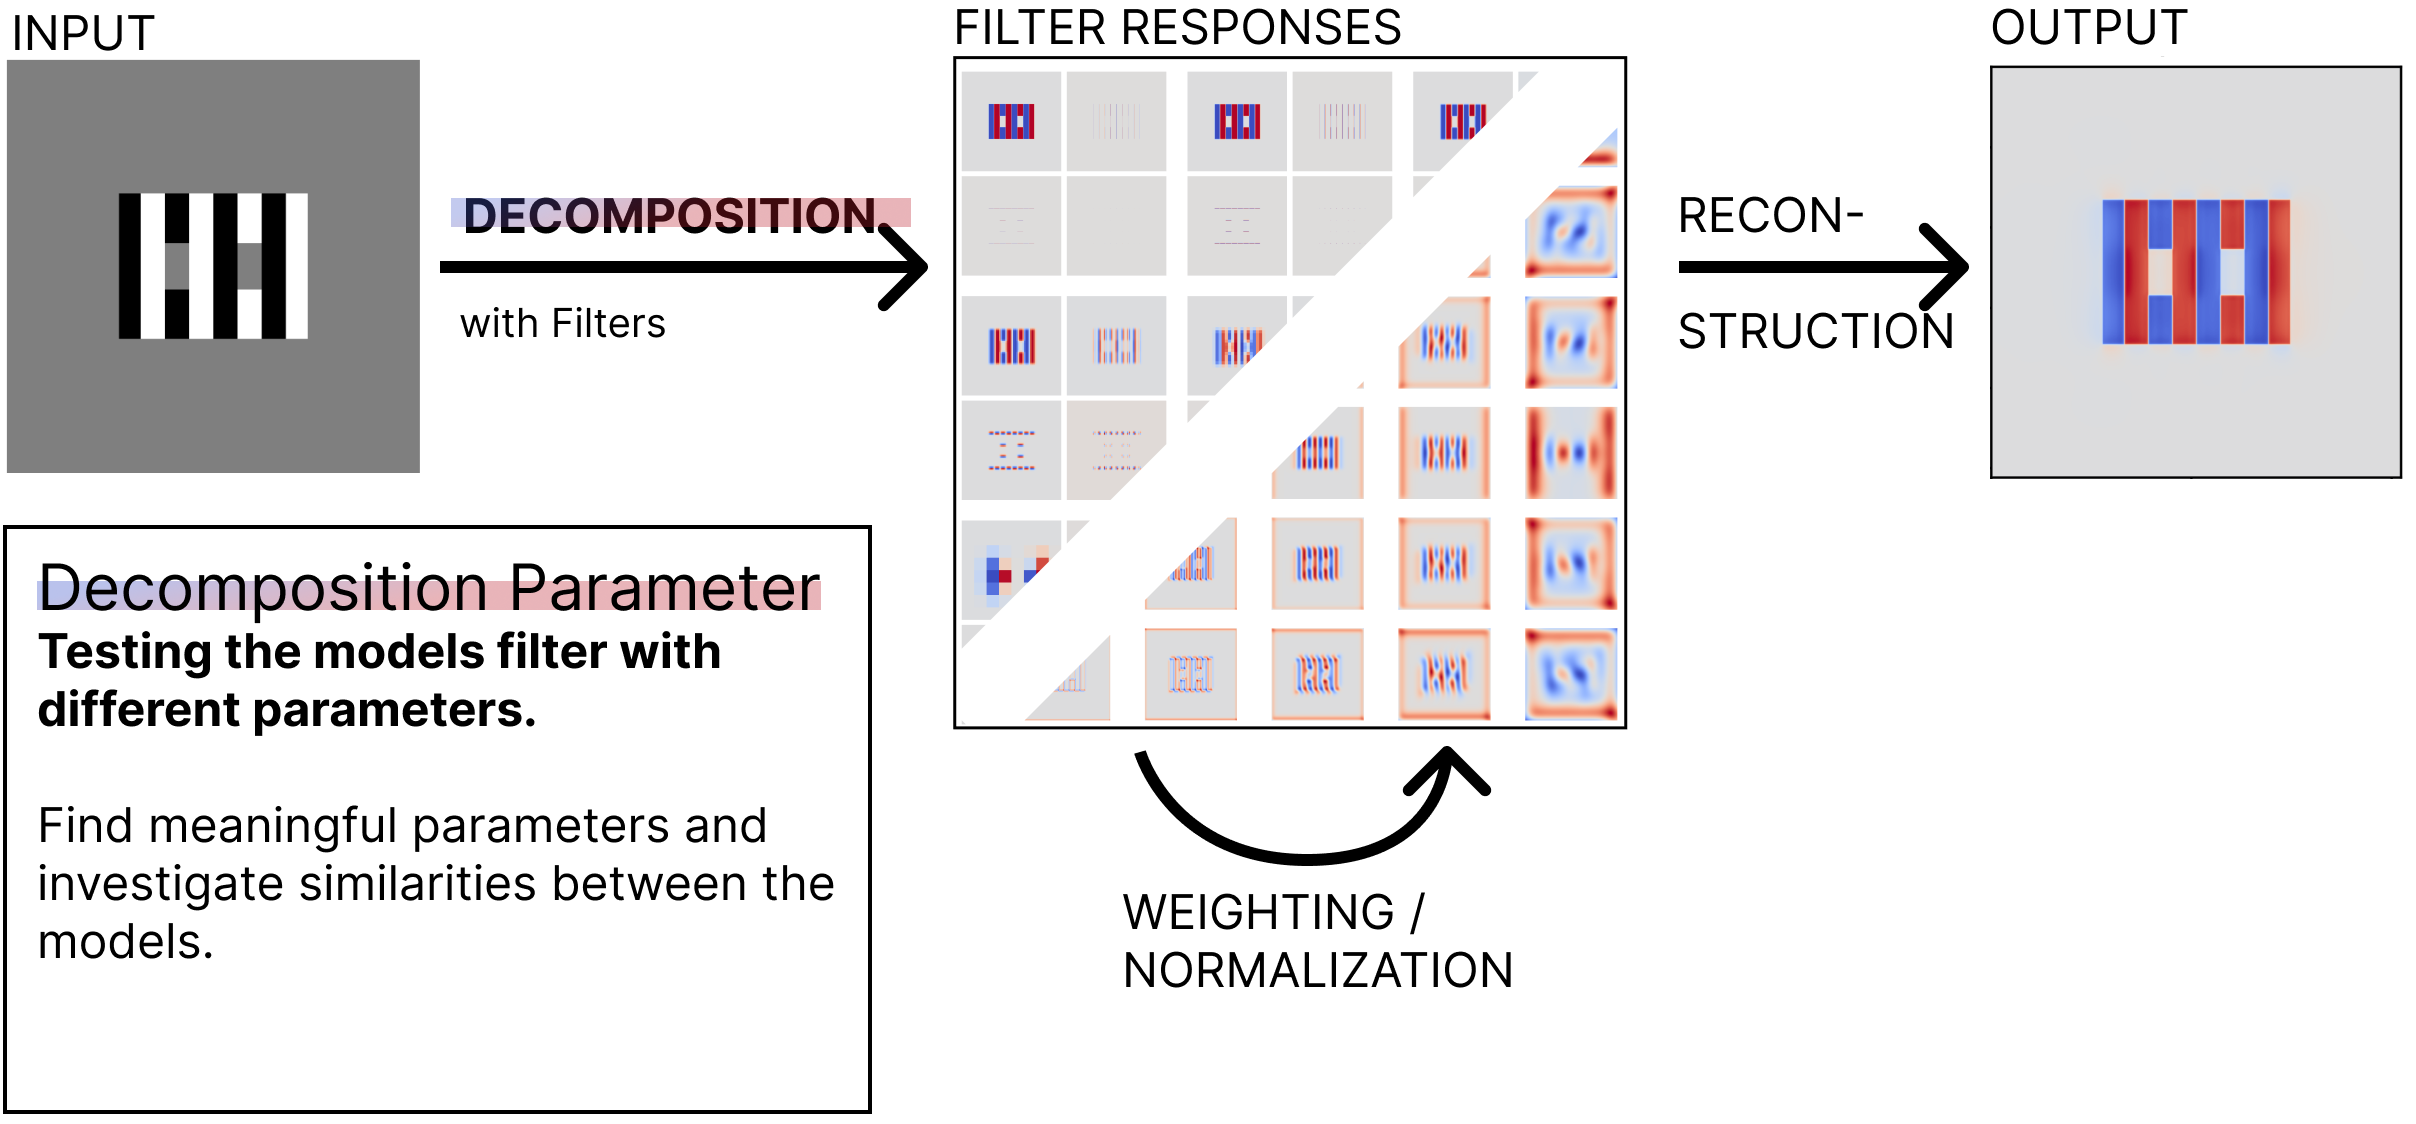
\includegraphics[width=\linewidth]{media/methodology/decomposition_overview.png}
    \begin{minipage}{0.8\textwidth}
    \caption{Methodology overview of filter testing}
    \label{fig:figure11}
    \end{minipage}
\end{figure}
Previously, we established a baseline of the ODOG and BIWaM responses under their default
configurations. Building on this foundation, we now analyze their correlating parameters
in the decomposition stage to identify how changes affect model predictions compared to
the baseline.\\
\textcolor{red}{TODO: introduction into model mechanics and the concrete parameters}
\textbf{Parameters tested} \\
ODOG:
\begin{itemize} 
    \item Orientations: ODOG uses oriented filter spread across 0-180 degrees.
    The original model has 7 orientations.
    \item Scales: The filter bank’s scales define the amount of extracted
    spatial frequencies. The original model has 6 scales.
\end{itemize}

BIWaM:
\begin{itemize} 
    \item Wavelet Levels: The depth of the wavelet decomposition defines the
    amount of extracted spatial frequencies.
\end{itemize}

\textcolor{red}{TODO: go through parameter tests, show the effects}

\textcolor{red}{TODO: show that on few scales the models diverge, come to the hypothesis 
that the residula image accounts for that}

\textcolor{red}{TODO: outro is that we have a new baseline with aligned decomposition stage}

To ensure a fair comparison between the models in the next section:
\begin{itemize} 
    \item ODOG and BIWaM will be tested using same number of orientations and scales.
    \item BIWaM will be evaluated without the residual image.
\end{itemize}

\newpage
%_/_/_/_/_/_/_/_/_/_/_/_/_/_/_/_/_/_/_/_/_/_/_/_/_/_/_/_/_/_/
\section{Aligned models}

\begin{figure}[H]
    \centering
    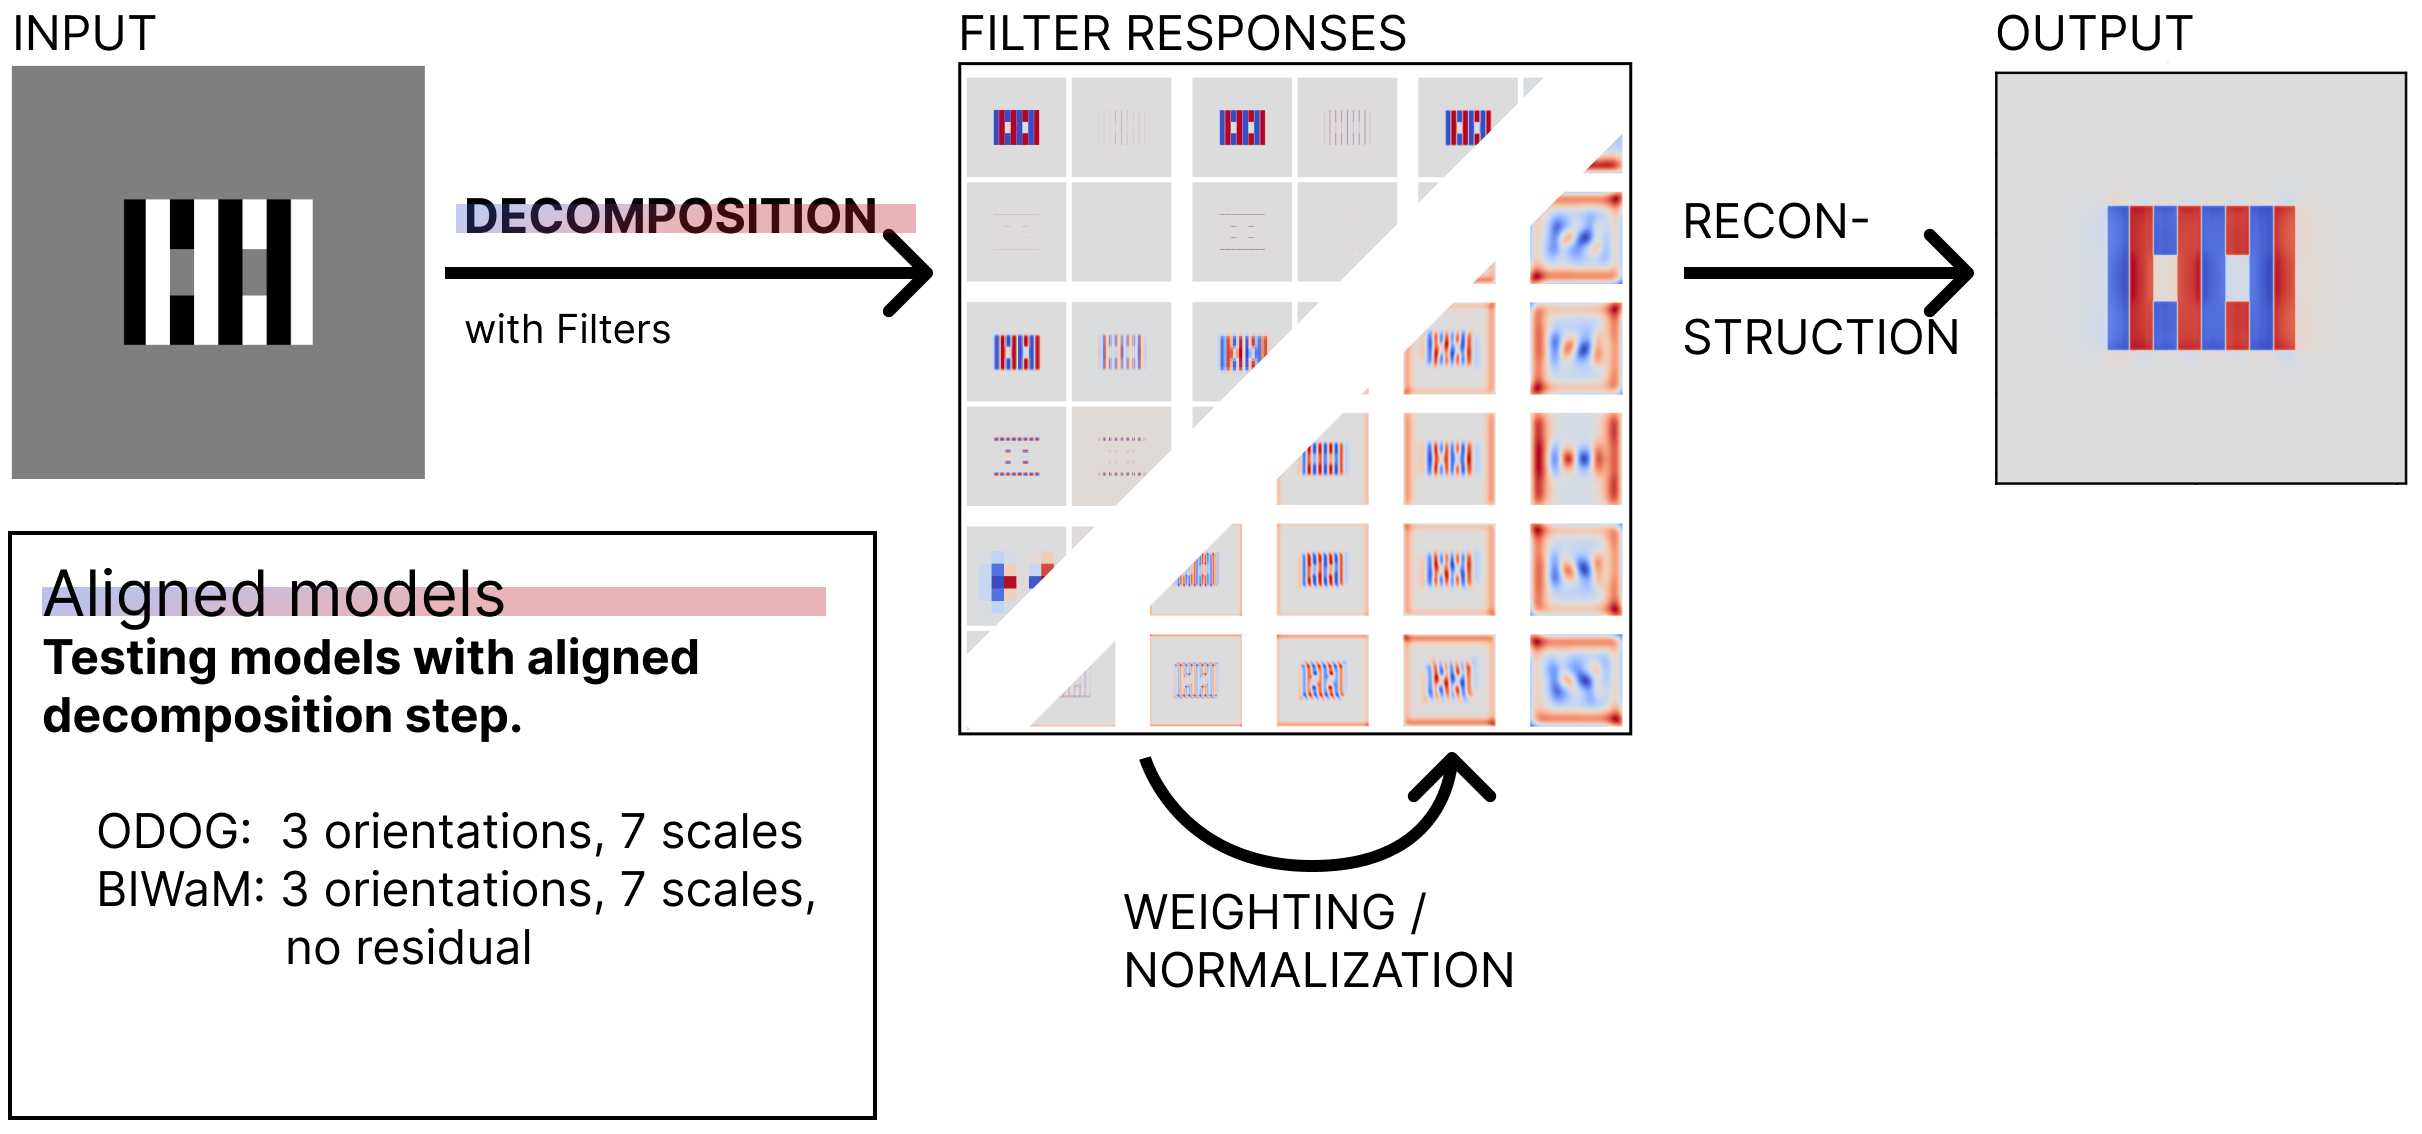
\includegraphics[width=\linewidth]{media/methodology/aligned_overview.png}
    \begin{minipage}{0.8\textwidth}
    \caption{Methodology overview of testing aligned models}
    \label{fig:figure12}
    \end{minipage}
\end{figure}

To compare ODOG and BIWaM in a fair setting, I evaluated both models on all seven test
stimuli with aligned decomposition stage as established in the previous section. The
parameters were set as follows: \\
ODOG:
\begin{itemize} 
    \item 7 scales
    \item 3 orientations
\end{itemize}
BIWaM:
\begin{itemize} 
    \item 7 wavelet levels
    \item No residual image
\end{itemize}

Each of the seven test stimulus was processed through both models with the aligned
parameters. The outputs were analyzed for changes in the response pattern, sensitivity to
features of the stimuli (e.g. edges, brightness) and the prediction of the illusion.

\textcolor{red}{TODO: go through tests on aligned models, show the effects of the
alignment and outline that the aligned models are getting closer.}

This comparison demonstrates that the decomposition stage of the models, when aligned,
exhibit similar overall behavior while retaining distinct characteristics based on the
following stages (weighting and normalization). These findings establish a baseline for
further alignments.

\newpage
%_/_/_/_/_/_/_/_/_/_/_/_/_/_/_/_/_/_/_/_/_/_/_/_/_/_/_/_/_/_/
\section{CSF weighting}

\begin{figure}[H]
    \centering
    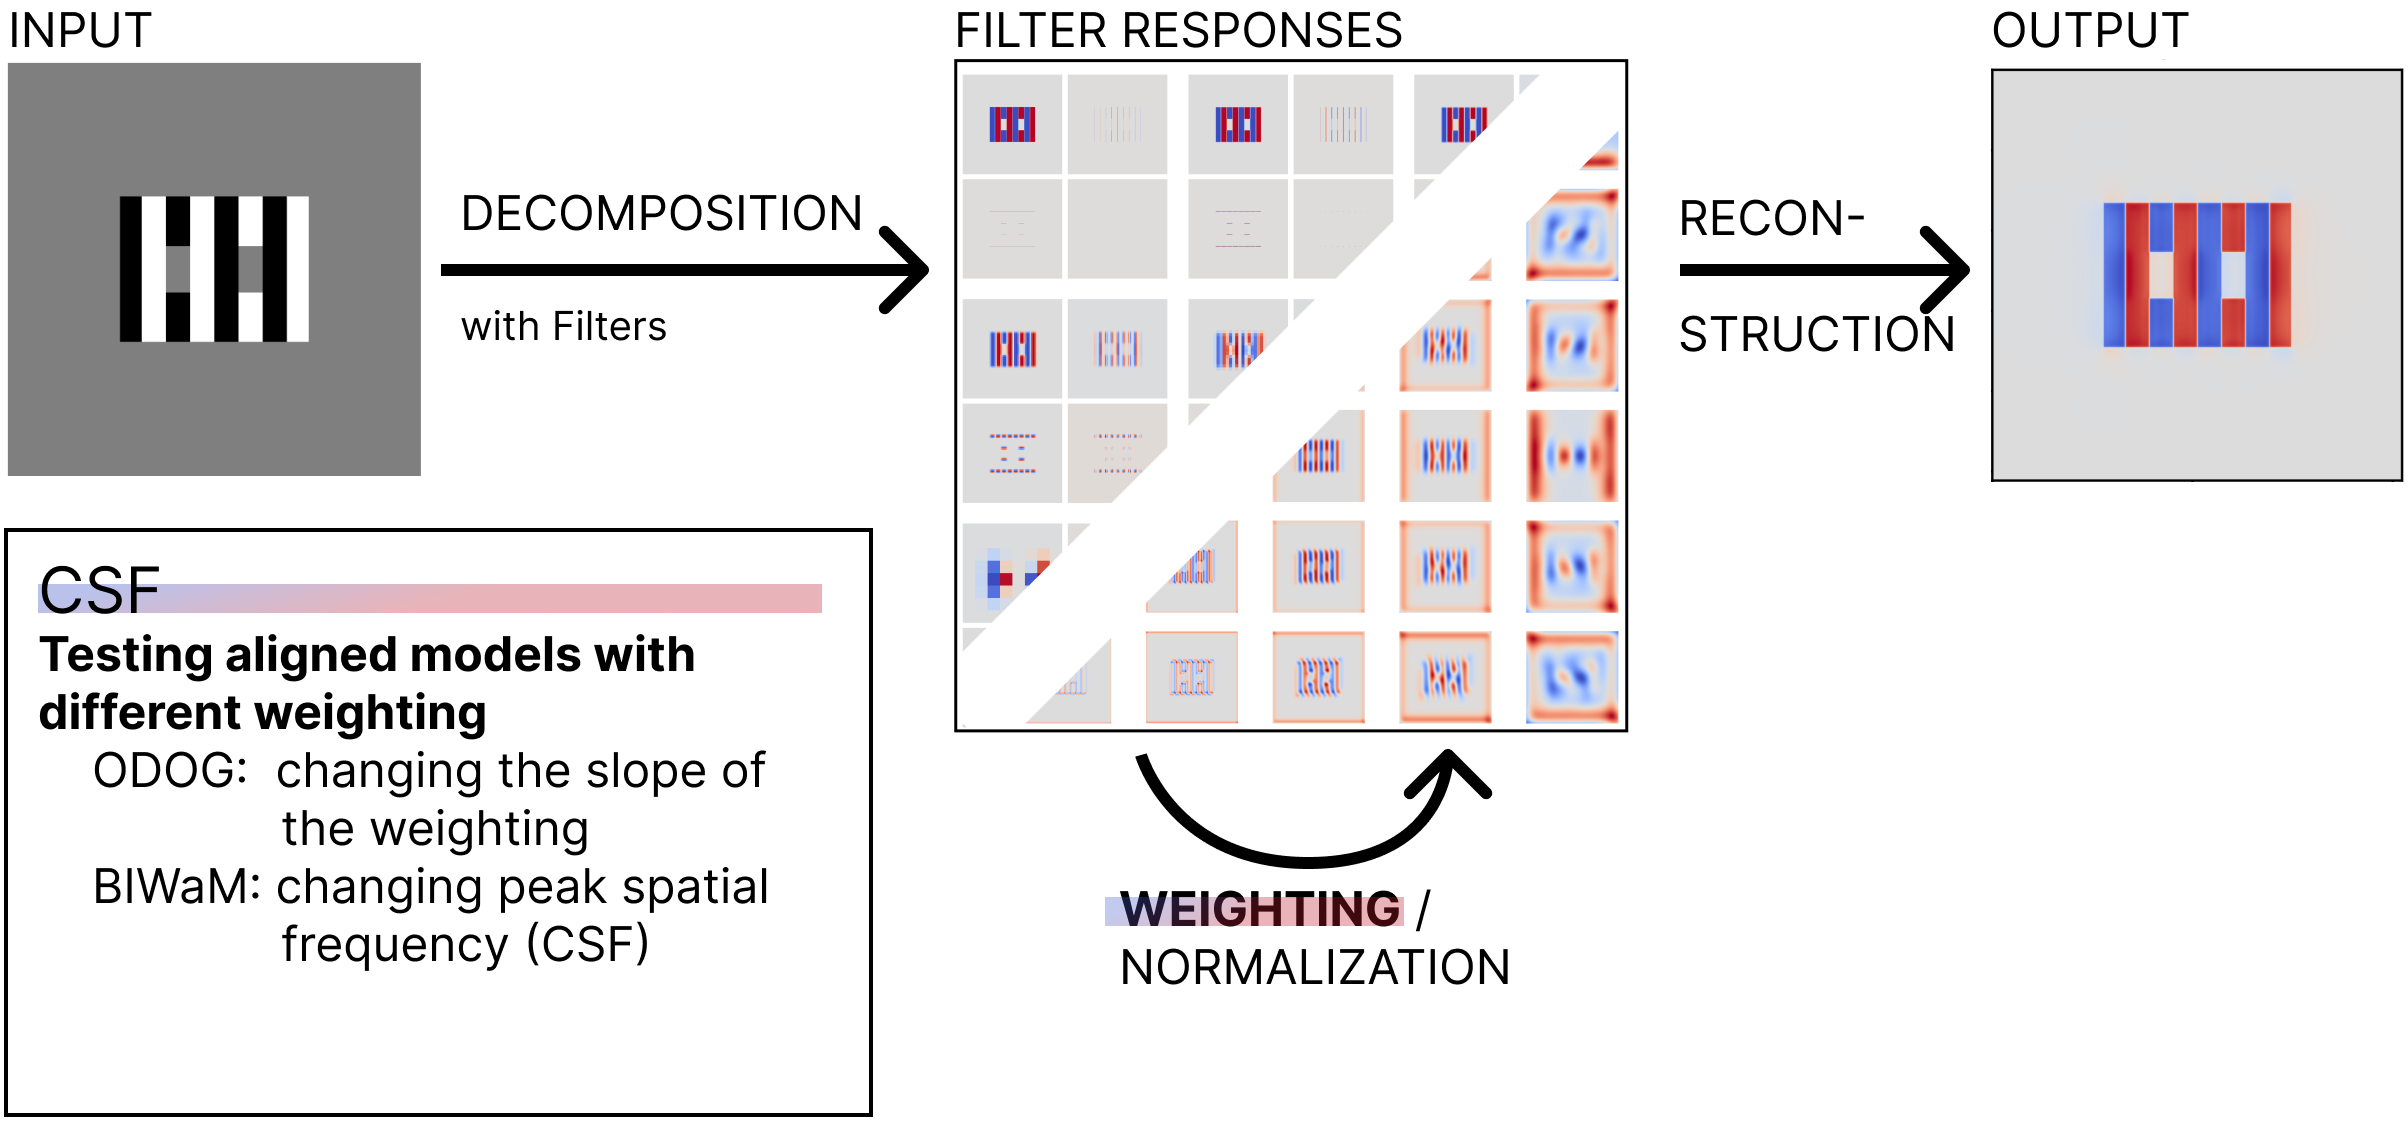
\includegraphics[width=\linewidth]{media/methodology/csf_overview.png}
    \begin{minipage}{0.8\textwidth}
    \caption{Methodology overview of CSF testing}
    \label{fig:figure13}
    \end{minipage}
\end{figure}

With the models aligned at the decomposition stage, the next step involves analyzing their
weighting mechanisms for frequency channels. Both models incorporate mechanisms to weight
spatial frequencies, inspired by the characteristics of the Contrast Sensitivity Function
(CSF) in human vision and can be accessed in the source code.\\
\textbf{Parameters tested} \\
ODOG:
\begin{itemize} 
    \item Slope in Weighting Step: This parameter defines the slope of a linear function
    around 1, where lower frequencies are attenuated (factor < 1), and higher frequencies
    are enhanced (factor > 1). The weighting follows a pattern similar to the CSF, since
    the scales are spaced logarithmically and therefore the linear function effectively is
    the positive side of a gaussian.
\end{itemize}
BIWaM:
\begin{itemize} 
    \item Peak\_SF: This parameter shifts the peak of the CSF function along the x-axis.
    The CSF is modeled using two Gaussians, allowing the model to enhance lower or higher
    frequencies based on the value of Peak\_SF.
\end{itemize}

\textcolor{red}{TODO: go through both tests on aligned models, show the effects of the
different weightings.}

\newpage
%_/_/_/_/_/_/_/_/_/_/_/_/_/_/_/_/_/_/_/_/_/_/_/_/_/_/_/_/_/_/
\section{Spatial interaction}

\begin{figure}[H]
    \centering
    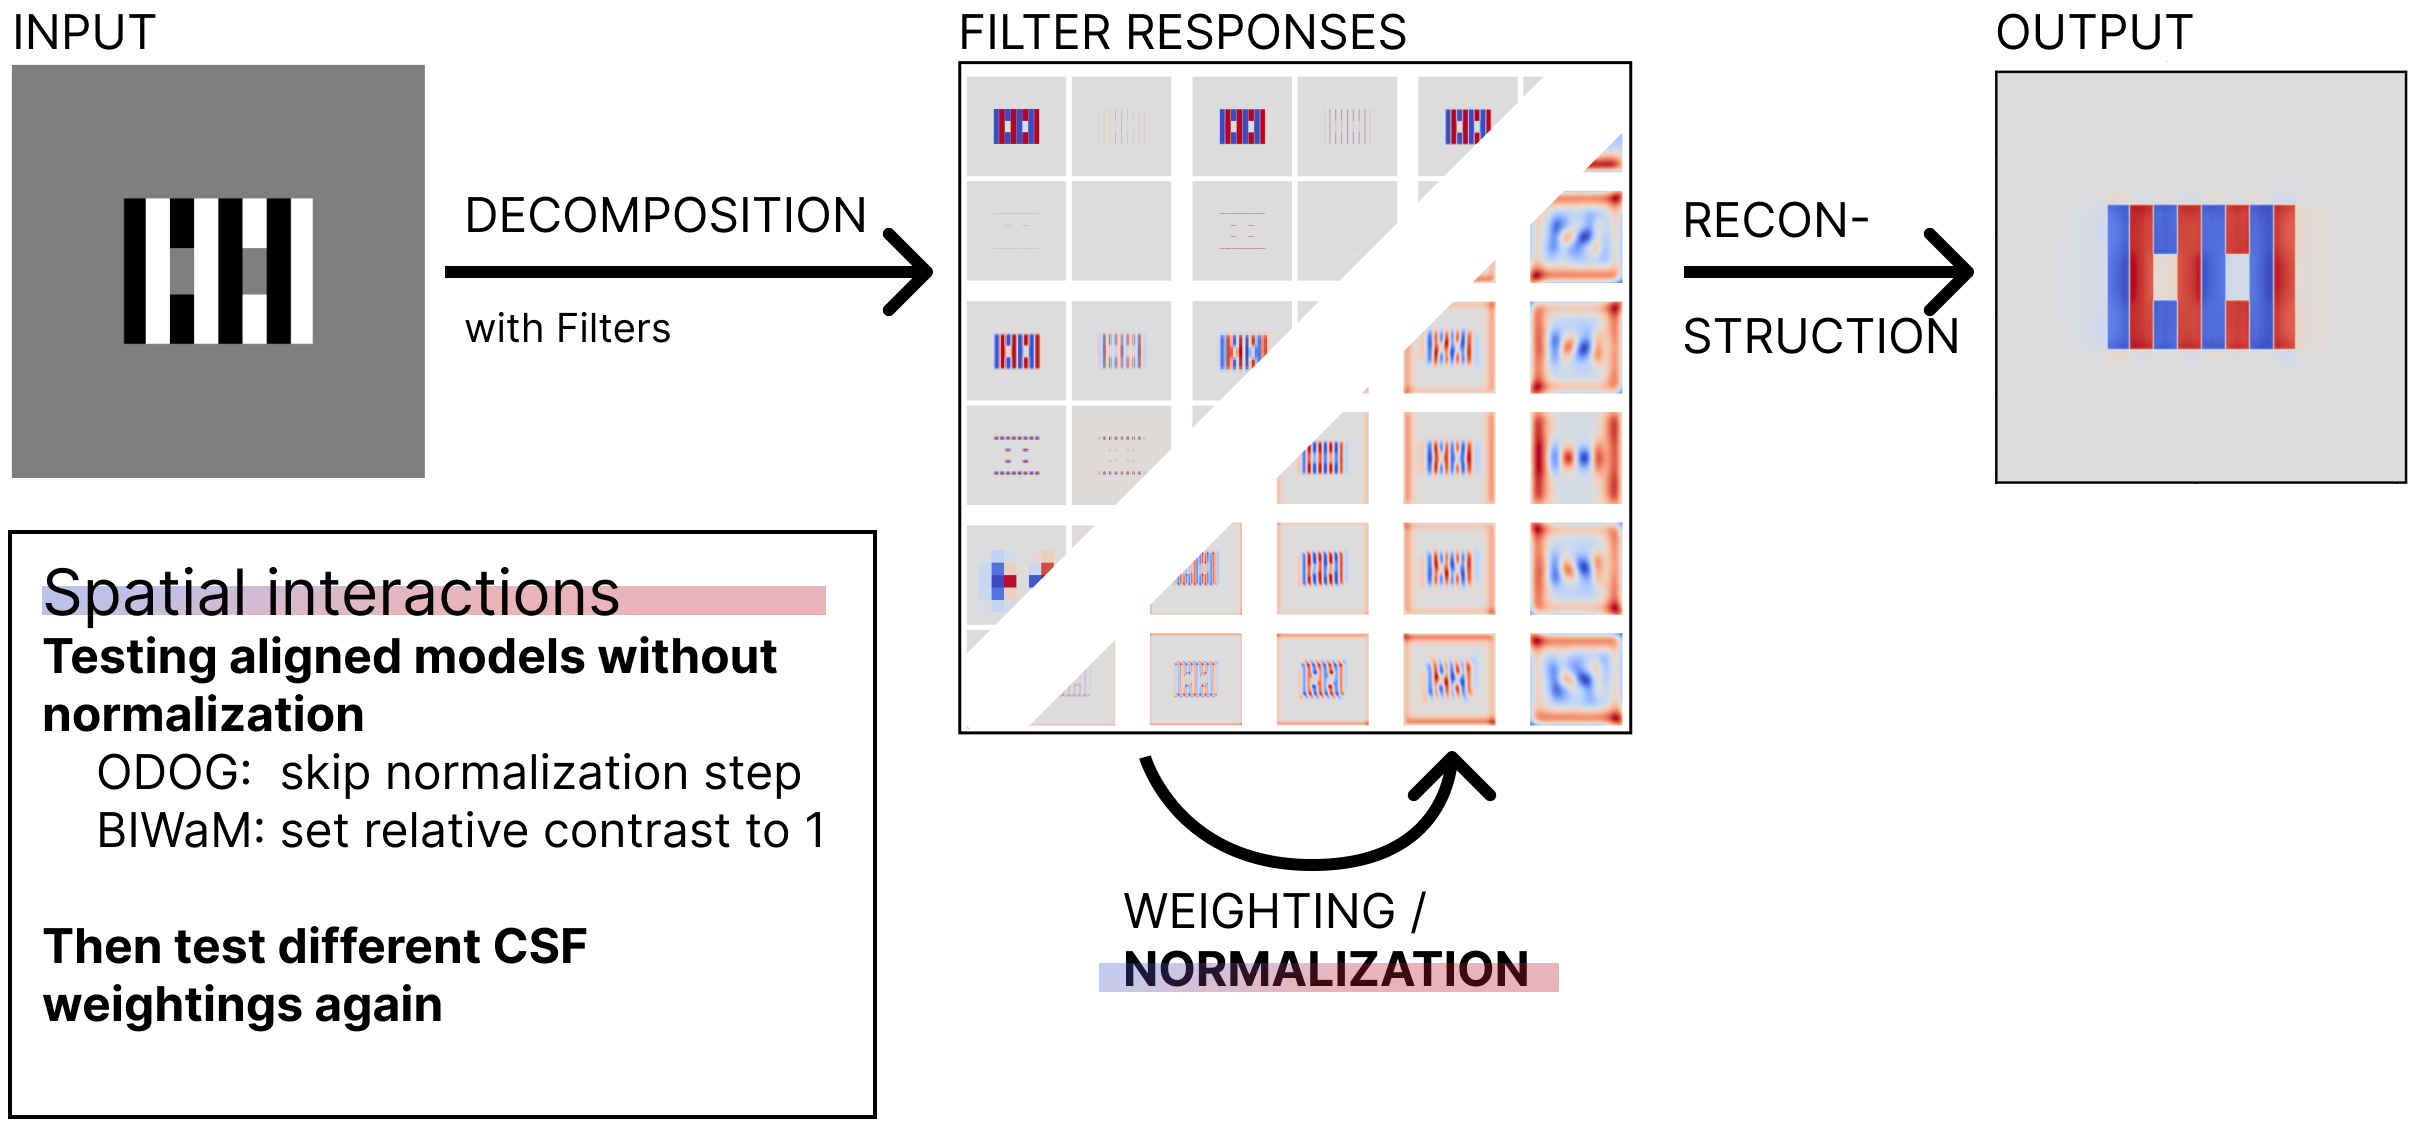
\includegraphics[width=\linewidth]{media/methodology/spatial_interaction_overview.png}
    \begin{minipage}{0.8\textwidth}
    \caption{Methodology overview of testing models without spatial interaction}
    \label{fig:figure14}
    \end{minipage}
\end{figure}

The final analysis focuses on the spatial interaction mechanisms of the models,
implemented through normalization processes. To evaluate the importance of normalization,
the models were tested with this feature disabled. To confirm the role of normalization,
the models were also tested with different CSF weightings as used in the previous section.
This helped determine whether CSF weighting alone could account for the models’ behavior
in the absence of normalization.

ODOG:
\begin{itemize} 
    \item The normalization step was skipped entirely.
\end{itemize}
BIWaM:
\begin{itemize} 
    \item The relative contrast was set to 1, effectively disabling normalization.
\end{itemize}

\textcolor{red}{TODO: go through the tests on aligned models without normalization, show
the effects of it and then go through CSF test without normalization again.}

This analysis underscores the critical role of normalization in brightness prediction. It
also highlights the limitations of frequency weighting alone, emphasizing the need for
both (if previous section also shows need for CSF) mechanisms to achieve robust and
realistic model behavior.



% For each step shown in Figure \ref{fig:figure7}, the focus will be on the structural
% differences between the models. Adjusting the ODOG model to align it more closely with the
% BIWaM model, will reveal their importance step by step, shown in the diagram of Figure
% \ref{fig:figure14}. The plan is to modify the source code for each part listed in the table
% of Figure \ref*{fig:figure14} and to conclude every change by running the models with the
% modification on a set of illusions and comparing the outputs quantitatively.

% \begin{figure}[H]
%     \centering
%     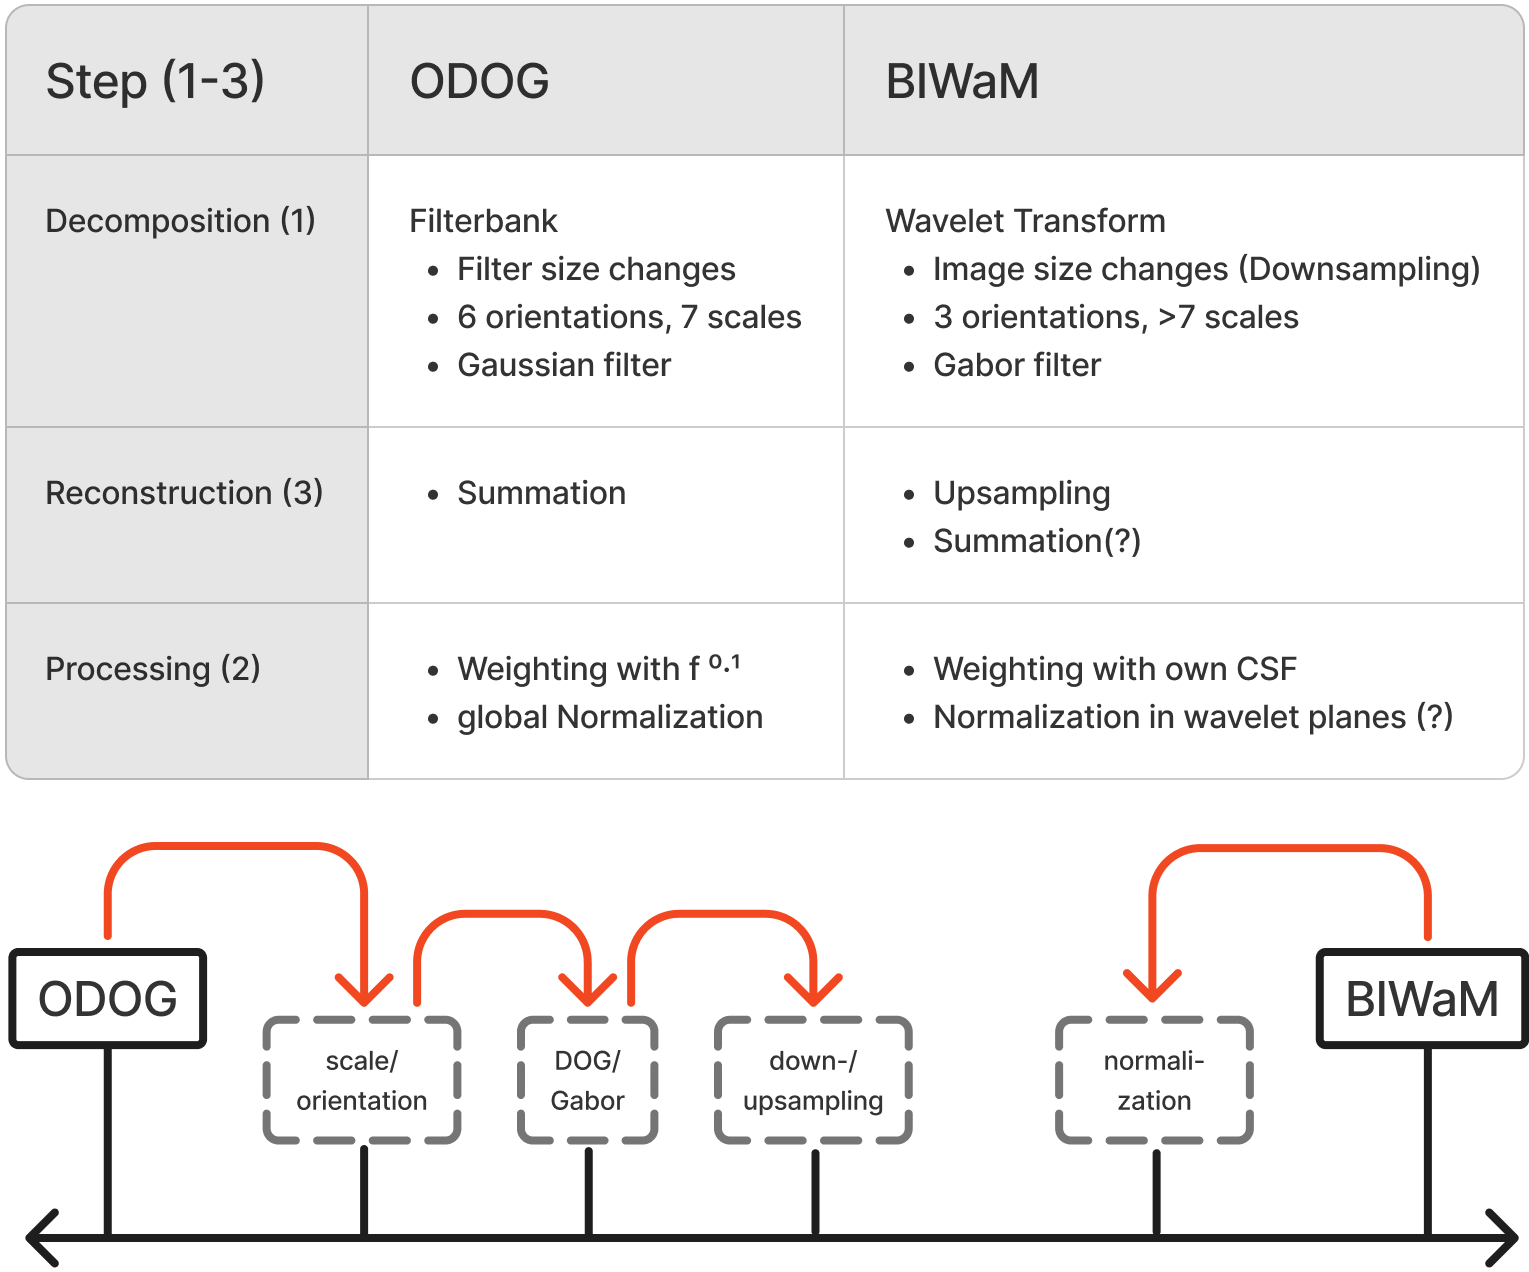
\includegraphics[width=\linewidth]{media/table_differences.png}
%     \begin{minipage}{0.8\textwidth}
%     \caption{The table shows the already known differences between the models for each of
%     the steps (1-3). The diagram below shows how i plan to narrow down the search for
%     differences. By adjusting the models for each of the steps shown and concluding the
%     impact by comparing the output, I wat to isolate the differences with the most
%     impact.}
%     \label{fig:figure14}
%     \end{minipage}
% \end{figure}


\newpage

% \section{Results} 
% \begin{enumerate}
%     \item \textbf{Recreation of published predictions for BIWaM}:
%     \begin{itemize}
%         \item Avilable Matlab implementation is another version (CIWaM).
%         \item Bad reproducibility led to extensive research and parameter exploration.
%         \item DWT function is highly optimized and undocumented -> took a lot of time to understand.
%         \item Python reimplementation behaves same as Matlab version (CIWaM).
%         \item Using CIWaM\_per\_channel function from CIWaM code as BIWaM representative.
%         \item \textbf{Predictions}
%             \begin{itemize} 
%                 \item Available BIWaM predicts brightness illusions qualitatively, but not quantitatively.
%                 \item Model outputs diverged from published results despite wide parameter adjustments.
%                 \item This led to the question of whether the available model is different, or whether the parameters are different, or whether the re-created stimuli (as input) are different.
%                 \item Tests indicated high robustness of BIWaM to input variations, suggesting that output differences are coming from differences in implementation rather than the re-created stimuli.
%             \end{itemize}
%     \end{itemize}

%     \item \textbf{Findings on parameter effects}:
%     \begin{itemize}
%         \item Adjusting wavelet levels influenced decomposition depth but did not resolve discrepancies.
%         \item Modifying filters results in ...
%         \item Modifying window size results in ...
%         \item Modifying peak s.f. results in ...
%     \end{itemize}

%     \item \textbf{Findings on comparative testing}:
%     \begin{itemize}
%         \item On the exact same stimuli the original models ....
%         \item With aligned parameters both models behave ...
%     \end{itemize}

%     \item \textbf{Potential differences between models}:
%     \begin{itemize}
%         \item Studying the models showed that the following features of the models are causing differences
%     \end{itemize}
% \end{enumerate}

\newpage

\section{Discussion} 
\begin{enumerate}
    \item \textbf{Linking differences in structure with results in behavior}
    \item ODOG is literally a Fourier decomposition. It gets a base frequency components
    and then its harmonics as the filters are logarithmic spaced. The magnitude of every
    component gets modified by CSF(slope)
    \item Resolution of image effects the models. link to hendrik
    \item Over-/Undershooting, log-gabor filter as better filter for both models. 
    \item \textbf{Insights into decomposition}:
    \begin{itemize}
        \item Information loss through downsampling is compensated due to residual image.
    \end{itemize}
    \item Speed of models
\end{enumerate}

\newpage
\listoffigures

\newpage
\nocite{Adelson1996}
\nocite{Brainard2003-BRACCD-2}
\nocite{Hanson1978}
\nocite{Murray2021}
\nocite{Kingdom2014}
\nocite{Robinson2007}
\vspace*{1cm}
%Literatur
\begin{minipage}{1\textwidth}
\printbibliography
\end{minipage}


\end{document}
